\documentclass[11pt,a4paper]{article}
\usepackage[T1]{fontenc}
\usepackage{lmodern}
\usepackage[margin=28mm,top=25mm,bottom=25mm]{geometry}
\usepackage{amsmath,amssymb,amsthm}
\usepackage{microtype,tikz,needspace}
\usetikzlibrary{arrows.meta,decorations.markings}
\usepackage[hidelinks]{hyperref}
\hypersetup{bookmarksdepth=3,pdftitle={Bimodule String Diagrams and the Generalized Mackey Decomposition},pdfauthor={Ian Xiao}}
\setlength{\emergencystretch}{1.5em}
\setlength{\textfloatsep}{14pt plus 3pt minus 3pt}
\setlength{\intextsep}{13pt plus 3pt minus 3pt}
\raggedbottom
\setlength{\parindent}{0pt}
\setlength{\parskip}{3pt plus 1pt}
\numberwithin{equation}{section}
\setcounter{tocdepth}{2}

\newtheorem{theorem}{Theorem}[section]
\newtheorem{proposition}[theorem]{Proposition}
\newtheorem{lemma}[theorem]{Lemma}
\newtheorem{corollary}[theorem]{Corollary}
\theoremstyle{definition}
\newtheorem{example}{Example}[section]
\newcommand{\C}{\mathbb C}
\newcommand{\Mod}{\text{-}\mathrm{Mod}}
\newcommand{\Bimod}{\operatorname{Bimod}}
\newcommand{\Hom}{\operatorname{Hom}}
\newcommand{\End}{\operatorname{End}}
\newcommand{\op}{\mathrm{op}}
\newcommand{\id}{\mathrm{id}}
\newcommand{\Ind}{\operatorname{Ind}}
\newcommand{\Res}{\operatorname{Res}}
\newcommand{\co}[1]{\overline{#1}}
\newcommand{\cg}[2]{{}^{#1}\!#2}
\newcommand{\I}{\mathsf I}
\newcommand{\D}{\mathsf D}
\newcommand{\ev}{\varepsilon}
\newcommand{\tv}{\widetilde{\varepsilon}}
\newcommand{\tu}{\widetilde{\eta}}
\tikzset{
  wire/.style={line width=.9pt,line cap=round},
  oriented/.style={wire,decoration={markings,mark=at position .57 with {\arrow{Stealth[length=5pt,width=5pt]}}},postaction={decorate}},
  region/.style={font=\normalsize,inner sep=1.5pt,outer sep=0pt},
  strandlabel/.style={font=\normalsize,inner sep=1.5pt,outer sep=0pt}
}
\newcommand{\adjdiag}[7]{%
  \begin{tikzpicture}[x=1cm,y=1cm,baseline=-.60cm]
  \useasboundingbox (-2.0,-1.36) rectangle (2.0,1.08);
  \draw[oriented] #1;
  \draw[oriented] #2;
  \node[region] at (-1.45,#3) {$#4$};
  \node[region] at (0,#3) {$#5$};
  \node[region] at (1.45,#3) {$#4$};
  \node[strandlabel,anchor=east] at (-.74,0) {$\co\alpha$};
  \node[strandlabel,anchor=west] at (.74,0) {$\co\alpha$};
  \node[region] at (0,#6) {$#7$};
  \end{tikzpicture}%
}

% Diagrams for compositions of two crossings.
\tikzset{
  reverseoriented/.style={
    wire,decoration={markings,mark=at position .57 with
       {\arrowreversed{Stealth[length=5pt,width=5pt]}}},postaction={decorate}},
  arrowatend/.style={wire,-{Stealth[length=5pt,width=5pt]}},
  arrowatstart/.style={wire,{Stealth[length=5pt,width=5pt]}-}
}
\newcommand{\mackeytwocrossings}[4]{%
 \begin{tikzpicture}[baseline=(current bounding box.center),x=1cm,y=1cm]
   \draw[#4] (.78,-1.37)
     .. controls (.10,-.96) and (-1.04,-.45) .. (-1.04,0)
     .. controls (-1.04,.43) and (.10,.96) .. (.78,1.37);
   \draw[#4] (-.78,1.37)
     .. controls (-.10,.96) and (1.04,.45) .. (1.04,0)
     .. controls (1.04,-.43) and (-.10,-.96) .. (-.78,-1.37);
   \node[region] at (0,1.22) {$#1$};
   \node[region] at (0,0) {$#2$};
   \node[region] at (0,-1.22) {$#3$};
   \node[region] at (-1.39,0) {$K$};
   \node[region] at (1.39,0) {$H$};
 \end{tikzpicture}%
}
\newcommand{\mackeyidentity}[5]{%
 \begin{tikzpicture}[baseline=(current bounding box.center),x=1cm,y=1cm]
   \draw[#4] (-.76,-.95)--(-.76,.95);
   \draw[#5] (.76,-.95)--(.76,.95);
   \node[region] at (-1.27,0) {$K$};
   \node[region] at (0,0) {$#1$};
   \node[region] at (1.27,0) {$H$};
   \node[strandlabel] at (-.76,-1.23) {$#2$};
   \node[strandlabel] at (.76,-1.23) {$#3$};
 \end{tikzpicture}%
}

% The main curve continues through both dots. The outer curves
% meet it tangentially, as in the handwritten diagrams.
\tikzset{
  mackeyup/.style={arrowatend,decoration={
    markings,mark=at position .075 with
      {\arrow{Stealth[length=5pt,width=5pt]}}},postaction={decorate}}
}
\newcommand{\mackeyendomorphism}[1]{%
 \begin{tikzpicture}[baseline=(current bounding box.center),x=1cm,y=.95cm]
   \coordinate (upperleft) at (-.57,.48);
   \coordinate (lowerleft) at (-.59,-.48);
   \coordinate (upperright) at (1.12,1.64);
   \coordinate (lowerright) at (1.07,-1.64);
   \coordinate (upperdot) at (.24,1.04);
   \coordinate (lowerdot) at (.23,-1.09);

   % Continuous beta-to-beta curve through the two dots.
   \draw[mackeyup] (1.54,-3.16)
     .. controls (1.52,-2.59) and (1.33,-2.01) .. (lowerright)
     .. controls (.83,-1.39) and (.50,-1.28) .. (lowerdot)
     .. controls (-.05,-.88) and (-.32,-.67) .. (lowerleft)
     .. controls (-.80,-.33) and (-1.03,-.16) .. (-.96,.02)
     .. controls (-.89,.20) and (-.76,.36) .. (upperleft)
     .. controls (-.34,.64) and (-.02,.85) .. (upperdot)
     .. controls (.56,1.26) and (.90,1.35) .. (upperright)
     .. controls (1.44,2.07) and (1.55,2.71) .. (1.74,3.16);
   \draw[oriented] (-1.68,3.20) -- (-1.68,.72)
     .. controls (-1.68,.42) and (-1.60,.29) .. (-1.35,.28)
     .. controls (-1.10,.27) and (-.87,.28) .. (upperleft);
   \draw[arrowatend] (lowerleft)
     .. controls (-.84,-.31) and (-1.29,-.27) .. (-1.46,-.47)
     .. controls (-1.73,-.80) and (-1.69,-2.34) .. (-1.79,-3.14);
   \draw[oriented] (upperright)
     .. controls (1.39,1.99) and (1.68,2.17) .. (1.88,1.94)
     .. controls (2.03,1.76) and (2.04,1.37) .. (2.04,1.05)
     -- (2.11,-1.53)
     .. controls (2.12,-2.03) and (1.83,-2.14) .. (1.49,-1.94)
     .. controls (1.34,-1.85) and (1.19,-1.77) .. (lowerright);

   \fill (upperdot) circle (2pt);
   \fill (lowerdot) circle (2pt);
   \node[strandlabel,anchor=south east] at (.21,1.16) {$\sigma_{#1}$};
   \node[strandlabel,anchor=south west] at (.39,-1.02) {$\sigma_{#1}^{-1}$};
   \node[strandlabel,anchor=east] at (-1.87,3.18) {$\bar\alpha$};
   \node[strandlabel,anchor=north] at (-1.86,-3.32) {$\bar\alpha$};
   \node[strandlabel,anchor=west] at (1.92,3.20) {$\bar\beta$};
   \node[strandlabel,anchor=west] at (1.73,-3.19) {$\bar\beta$};
   \node[strandlabel,anchor=west] at (-.70,-.03) {$\overline{\alpha^{-1}}$};
   \node[strandlabel,anchor=west] at (2.31,-.78)
       {$\overline{\beta^{-1}\sigma_{#1}^{-1}}$};

   \node[region] at (-2.61,-.04) {$K$};
   \node[region] at (2.91,.12) {$H$};
   \node[region] at (-.56,2.34) {$G$};
   \node[region] at (-.58,-2.46) {$G$};
   \node[region] at (.71,.23) {$L_{#1}$};
 \end{tikzpicture}%
}
\newcommand{\mackeyorthogonality}[2]{%
 \begin{tikzpicture}[baseline=(current bounding box.center),x=1cm,y=.95cm]
   \coordinate (upperleft) at (-.47,1.77);
   \coordinate (lowerleft) at (-.55,-1.78);
   \coordinate (upperright) at (.52,.87);
   \coordinate (lowerright) at (.44,-.95);
   \coordinate (upperdot) at (-.05,1.37);
   \coordinate (lowerdot) at (-.15,-1.35);

   % Continuous inclusion-to-projection curve through the two dots.
   \draw[mackeyup] (-1.01,-3.17)
     .. controls (-.96,-2.62) and (-.72,-2.19) .. (lowerleft)
     .. controls (-.42,-1.58) and (-.29,-1.47) .. (lowerdot)
     .. controls (.05,-1.17) and (.22,-1.10) .. (lowerright)
     .. controls (.72,-.75) and (1.02,-.37) .. (.99,-.08)
     .. controls (.96,.20) and (.72,.59) .. (upperright)
     .. controls (.33,1.09) and (.15,1.15) .. (upperdot)
     .. controls (-.17,1.51) and (-.32,1.66) .. (upperleft)
     .. controls (-.83,2.03) and (-.72,2.67) .. (-.99,3.17);
   \draw[oriented] (upperleft)
     .. controls (-.77,1.98) and (-1.03,2.20) .. (-1.37,1.98)
     .. controls (-1.79,1.70) and (-1.82,1.44) .. (-1.81,.81)
     -- (-1.79,-1.01)
     .. controls (-1.77,-1.73) and (-1.65,-2.07) .. (-1.32,-2.16)
     .. controls (-1.09,-2.22) and (-.77,-1.98) .. (lowerleft);
   \draw[oriented] (1.75,3.21) -- (1.74,1.12)
     .. controls (1.74,.75) and (1.63,.65) .. (1.37,.61)
     .. controls (1.02,.55) and (.77,.63) .. (upperright);
   \draw[arrowatend] (lowerright)
     .. controls (.82,-.69) and (1.29,-.39) .. (1.48,-.55)
     .. controls (1.65,-.70) and (1.62,-1.12) .. (1.64,-1.53)
     -- (1.75,-3.13);

   \fill (upperdot) circle (2pt);
   \fill (lowerdot) circle (2pt);
   \node[strandlabel,anchor=south west] at (.09,1.46) {$\sigma_{#2}^{-1}$};
   \node[strandlabel,anchor=north west] at (-.06,-1.53) {$\sigma_{#1}$};
   \node[strandlabel,anchor=east] at (-1.14,3.22) {$\overline{\alpha^{-1}}$};
   \node[strandlabel,anchor=east] at (-1.17,-3.06) {$\overline{\alpha^{-1}}$};
   \node[strandlabel,anchor=west] at (1.97,3.12)
       {$\overline{\beta^{-1}\sigma_{#2}^{-1}}$};
   \node[strandlabel,anchor=west] at (1.97,-2.84)
       {$\overline{\beta^{-1}\sigma_{#1}^{-1}}$};
   \node[strandlabel,anchor=east] at (-2.04,.52) {$\bar\alpha$};
   \node[strandlabel] at (.57,-.04) {$\bar\beta$};

   \node[region] at (-2.59,-.44) {$K$};
   \node[region] at (2.47,-.38) {$H$};
   \node[region] at (-.78,.10) {$G$};
   \node[region] at (.27,2.91) {$L_{#2}$};
   \node[region] at (.31,-2.98) {$L_{#1}$};
 \end{tikzpicture}%
}

\title{\textbf{Bimodule String Diagrams and the\\Generalized Mackey Decomposition}}
\author{Ian Xiao}
\date{}

% Diagrams for the mixed orientations in Section 6.
\newcommand{\mixedThreeWires}[3]{%
  \draw[#1] (0,0)--(0,.26)
    .. controls (0,.73) and (1.4,.91) .. (1.4,1.45)
    --(1.4,1.79)
    .. controls (1.4,2.33) and (2.8,2.47) .. (2.8,3.01)
    --(2.8,4.8);
  \draw[#2] (1.4,0)--(1.4,.26)
    .. controls (1.4,.73) and (0,.91) .. (0,1.45)
    --(0,3.35)
    .. controls (0,3.89) and (1.4,4.03) .. (1.4,4.57)
    --(1.4,4.8);
  \draw[#3] (2.8,0)--(2.8,1.79)
    .. controls (2.8,2.33) and (1.4,2.47) .. (1.4,3.01)
    --(1.4,3.35)
    .. controls (1.4,3.89) and (0,4.03) .. (0,4.57)
    --(0,4.8);
}
\newcommand{\mixedThreeLeft}{%
  \foreach \x/\y/\i/\offset in {.7/.82875/1/-.43,2.1/2.4/2/.43,.7/3.96/3/-.43}{
    \fill (\x,\y) circle (1.9pt);
    \node[strandlabel] at ({\x+\offset},\y) {$x_{\i}$};
  }
  \node[region] at (.69,2.4) {$B$};
}
\newcommand{\mixedThreeRight}{%
  \foreach \x/\y/\i/\offset in {2.1/.82875/1/.43,.7/2.4/2/-.43,2.1/3.96/3/.43}{
    \fill (\x,\y) circle (1.9pt);
    \node[strandlabel] at ({\x+\offset},\y) {$y_{\i}$};
  }
  \node[region] at (2.11,2.4) {$B'$};
}
\newcommand{\mixedThreeBoundary}[7]{%
  \node[region] at (-.48,2.4) {$G$};
  \node[region] at (3.28,2.4) {$F$};
  \node[region] at (.70,.18) {$#1$};
  \node[region] at (2.10,.18) {$#2$};
  \node[region] at (.70,4.60) {$#3$};
  \node[region] at (2.10,4.60) {$#4$};
  \foreach \x/\lab in {#5} {\node[strandlabel] at (\x,-.35) {$\bar\lab$};}
  \foreach \x/\lab in {#6} {\node[strandlabel] at (\x,5.15) {$\bar\lab$};}
  \node[font=\normalsize] at (1.4,-.90) {Case #7};
}
\begin{document}
\maketitle
\begin{abstract}
\noindent
I develop a string-diagram calculus for group-algebra bimodules in which
centralizer cosets record the conjugation embeddings used in induction
and restriction. Explicit inclusion and projection maps give Mackey
decomposition for conjugate embeddings. I prove Reidemeister I and II
identities and construct fixed-boundary Reidemeister III replacements.
Some cases require sums, and others admit no replacement even by linear
combinations. For finite parabolic subgroups of \(S_\infty\), ordered
block matching gives explicit double-coset representatives and Mackey
summands. Parabolic intersections and joins give further identities. For
the move with a middle restriction strand, a stabilizer index determines
the attainable orbit coefficients on the right-hand shape over any
commutative coefficient ring.
\end{abstract}

\makeatletter
\begingroup
\fontsize{10pt}{10.5pt}\selectfont
\setlength{\parskip}{0pt}
\renewcommand*{\l@section}[2]{%
  \addvspace{.2em}%
  \@dottedtocline{1}{0em}{1.7em}{\bfseries #1}{\bfseries #2}}
\renewcommand*{\l@subsection}{\@dottedtocline{2}{1.7em}{2.6em}}
\tableofcontents
\endgroup
\makeatother

\Needspace{7\baselineskip}
\section{Bimodules and functors}

We define the strands and generating maps as group-algebra bimodules
and use Eilenberg--Watts to identify the corresponding functors and
natural transformations.
\Needspace{11\baselineskip}
\subsection{The Eilenberg--Watts correspondence}

For unital rings \(R,S\), \(R\Mod\) denotes the category of unital left
\(R\)-modules and \(\Bimod(S,R)\) the category of unital \(S\)-\(R\)
bimodules.

\begin{theorem}[Eilenberg--Watts \cite{watts,getcurious}]\label{thm:ew}
For unital rings \(R,S\), there is an equivalence from \(\Bimod(S,R)\)
to the category of additive, right-exact functors \(R\Mod\to S\Mod\)
that preserve all set-indexed coproducts, with natural transformations
as morphisms. It sends
\[
  B\longmapsto B\otimes_R-,\qquad f\longmapsto f\otimes_R\id .
\]
Its quasi-inverse sends \(F\) to \(F({}_R R)\) and \(\theta\) to
\(\theta_R\). For \(b\in F(R)\) and \(r\in R\), the right action is
\(br=F(\rho_r)(b)\), where \(\rho_r(x)=xr\). For composable bimodules
\(B\in\Bimod(S,R)\) and \(C\in\Bimod(T,S)\), composition corresponds to
\(C\otimes_S B\), and the identity corresponds to the regular bimodule.
\end{theorem}

For \(\C\)-algebras the equivalence identifies bimodules with equal
scalar actions with \(\C\)-linear functors of the stated kind.

Let \(\mathcal A,\mathcal E\) be locally small abelian categories with
all set-indexed coproducts and small projective generators \(P,Q\).
Here small means that \(\Hom(P,-)\) or \(\Hom(Q,-)\) preserves those
coproducts. Put \(R=\End_{\mathcal A}(P)^\op\) and
\(S=\End_{\mathcal E}(Q)^\op\). The Hom functors give equivalences
\(\mathcal A\simeq R\Mod\) and \(\mathcal E\simeq S\Mod\)
\cite[Chs.~8--10]{getcurious}. Theorem~\ref{thm:ew} then sends \(F\) to
\(\Hom_{\mathcal E}(Q,F(P))\), with actions
\[
 q^\op b p^\op=F(p)\circ b\circ q.
\]
A natural transformation acts by postcomposition with its component
at \(P\).

\subsection{The diagrammatic bimodule category}\label{sec:diagram-category}

Khovanov's graphical calculus for induction and restriction between finite
groups is the starting point for this construction \cite[\S~3.2]{khovanov}.

Fix a group \(U\). For \(X\le U\), write \(\C[X]\) for its complex group algebra.
If \(\cg{\alpha}{H}=\alpha H\alpha^{-1}\le G\), write
\(\alpha_*:\C[H]\to \C[G]\) for conjugation by \(\alpha\), extended linearly.
This map depends exactly on
\[
 \bar\alpha=\alpha C_U(H),\qquad
 C_U(H)=\{u\in U:uh=hu\text{ for all }h\in H\}.
\]
The centralizer in a strand label is taken for the source of its
embedding.
Thus an eligible conjugating element for a strand from \(H\) into \(G\)
satisfies \(\alpha H\alpha^{-1}\le G\); the strand records its
centralizer coset, and hence the embedding, rather than a chosen
representative.

The up and down strands below denote
\[
 \I_{\co\alpha}^{G,H}={}_{\C[G]}(\C[G])_{\alpha_*,\C[H]},\qquad
 \D_{\co\alpha}^{H,G}={}_{\C[H],\alpha_*}(\C[G])_{\C[G]}.
\]
The actions are \(x\cdot h=x\alpha h\alpha^{-1}\) on \(\I\) and
\(h\cdot x=\alpha h\alpha^{-1}x\) on \(\D\). Tensoring on the right
gives induction and restriction, respectively. The target group
is on the left. Read horizontal composition as tensor product over
the middle group and vertical composition from bottom to top.

\begin{center}
\begin{tikzpicture}[x=1cm,y=1cm]
 \draw[oriented] (0,-.82)--(0,.82);
 \node[region] at (-.78,0) {$G$};
 \node[region] at (.78,0) {$H$};
 \node at (0,-1.10) {$\co\alpha$};
 \node at (0,1.19) {$\I_{\co\alpha}^{G,H}$};
 \draw[oriented] (5,.82)--(5,-.82);
 \node[region] at (4.22,0) {$H$};
 \node[region] at (5.78,0) {$G$};
 \node at (5,-1.10) {$\co\alpha$};
 \node at (5,1.19) {$\D_{\co\alpha}^{H,G}$};
\end{tikzpicture}
\end{center}

\paragraph{Nodes.}
Let \(\co\alpha,\co\beta\) be two labels for embeddings of \(H\) into
\(G\). Choose \(\alpha'\in\co\alpha\) and \(\beta'\in\co\beta\) with
\(d=\alpha'(\beta')^{-1}\in G\). This determines a node
\[
 \I_{\co\alpha}^{G,H}\xrightarrow{\ \cdot d\ }\I_{\co\beta}^{G,H},
 \qquad x\longmapsto xd.
\]
The map respects the right action exactly when
\(\alpha_*(h)d=d\beta_*(h)\) for all \(h\in H\).
The possible group elements are \(G\cap\alpha C_U(H)\beta^{-1}\).
Changing representatives can change \(d\) and hence the map.
For the down strands the same \(d\) gives \(x\mapsto d^{-1}x\).

\begin{center}
\begin{tikzpicture}[x=1cm,y=1cm]
 \draw[oriented] (0,-1.0)--(0,-.08);
 \draw[oriented] (0,.08)--(0,1.0);
 \fill (0,0) circle (2.2pt);
 \node[anchor=west] at (.20,0) {$d=\alpha'(\beta')^{-1}$};
 \node at (-.72,0) {$G$};
 \node at (3.47,0) {$H$};
 \node at (0,-1.24) {$\co\alpha$};
 \node at (0,1.24) {$\co\beta$};
 \draw[oriented] (6.4,1.0)--(6.4,.08);
 \draw[oriented] (6.4,-.08)--(6.4,-1.0);
 \fill (6.4,0) circle (2.2pt);
 \node[anchor=west] at (6.60,0) {$d^{-1}=\beta'(\alpha')^{-1}$};
 \node at (5.68,0) {$H$};
 \node at (9.86,0) {$G$};
 \node at (6.4,-1.24) {$\co\alpha$};
 \node at (6.4,1.24) {$\co\beta$};
\end{tikzpicture}
\end{center}

\paragraph{Linear dot labels.}
We also allow a node to be a finite \(\C\)-linear combination of the
group-element nodes just defined. For fixed incoming and outgoing
labels, write
\[
 a=\sum_{d\in S}c_d d,\qquad c_d\in\C,\qquad
 S\subseteq G\cap\alpha C_U(H)\beta^{-1}\text{ finite}.
\]
Every supported group element must be eligible individually:
\(\alpha_*(h)d=d\beta_*(h)\) for every \(h\in H\).
On up strands this node acts by \(x\mapsto xa\). The corresponding
linear combination on down strands acts by
\[
 x\longmapsto\sum_{d\in S}c_d d^{-1}x.
\]
This extends the group-element rule linearly; it does not take a
multiplicative inverse of \(a\). A group-algebra element that
intertwines only after its terms are added need not be an eligible
single dot. Larger diagrams can realize further bimodule maps, as
in Proposition~\ref{prop:orbit-hom}.

A linear label occupies one marked node, including for a zero label.
Its coefficients and support do not change the drawing's shape.
An eligible node labelled \(1\) evaluates to the identity map of its
strand, while the drawing still has a dot. Expanding a label into
terms is an equality of evaluated linear combinations; it does not
replace one marked node by several successive nodes.

\paragraph{Cups and caps.}
Suppress the embedding and group labels on \(\I,\D\).
Each tensor product is over the group algebra of the middle region.
For \(\Ind_{\alpha_*}\dashv\Res_{\alpha_*}\), the unit and counit are
\[
 \begin{aligned}
   \eta &: \C[H]\longrightarrow \D\otimes_{\C[G]}\I,\qquad
      h\longmapsto \alpha_*(h)\otimes 1,\\
   \ev &: \I\otimes_{\C[H]}\D\longrightarrow \C[G],\qquad
      x\otimes y\longmapsto xy.
 \end{aligned}
\]
In the unit formula, \(\D\otimes_{\C[G]}\I\) identifies with \(\C[G]\) by multiplication.
Define the \(\C[H]\)-bimodule trace
\[
 E_\alpha(g)=
 \begin{cases}
 \alpha^{-1}g\alpha,&g\in\cg{\alpha}{H},\\
 0,&g\notin\cg{\alpha}{H},
 \end{cases}
 \qquad g\in G,
\]
and extend it linearly. When \([G:\cg{\alpha}{H}]<\infty\), choose
\(T\subseteq G\) with \(G=\bigsqcup_{t\in T}\cg{\alpha}{H}\,t\).
The reverse adjunction \(\Res_{\alpha_*}\dashv\Ind_{\alpha_*}\) has
unit and counit
\[
 \begin{aligned}
 \tu &: \C[G]\longrightarrow \I\otimes_{\C[H]}\D,\qquad
           g\longmapsto \sum_{t\in T}g t^{-1}\otimes t
                      =\sum_{t\in T}t^{-1}\otimes t g,\\
 \tv &: \D\otimes_{\C[G]}\I\longrightarrow \C[H],\qquad
           x\otimes y\longmapsto E_\alpha(xy).
 \end{aligned}
\]
Replacing \(t\) by \(\alpha_*(h)t\) leaves the balanced tensor
\(t^{-1}\otimes t\) unchanged. Right multiplication by \(g\in G\)
permutes the cosets \(\cg{\alpha}{H}t\), which proves the displayed
equality for \(\tu\). The dual-basis identities are
\[
 \sum_{t\in T}t^{-1}\alpha_*\bigl(E_\alpha(t x)\bigr)=x,
 \qquad
 \sum_{t\in T}\alpha_*\bigl(E_\alpha(x t^{-1})\bigr)t=x .
\]
For a basis element \(x\in G\), each identity has exactly one
nonzero term, by the decompositions using \(T\) and \(T^{-1}\).
They give the two reverse triangle identities. The trace cap is
defined at every index. The reverse unit displayed above is part of
the generating calculus at finite index.

\begin{center}
\begin{tabular}{@{}c@{\hspace{12mm}}c@{}}
\adjdiag{(-.72,.64) .. controls (-.72,-.21) and (-.28,-.57) .. (0,-.57)}
{(0,-.57) .. controls (.28,-.57) and (.72,-.21) .. (.72,.64)}{.94}{H}{G}{-.94}{H}
&
\adjdiag{(-.72,-.94) .. controls (-.72,-.09) and (-.28,.27) .. (0,.27)}
{(0,.27) .. controls (.28,.27) and (.72,-.09) .. (.72,-.94)}{-1.22}{G}{H}{.64}{G}\\[-.5ex]
\(\eta\) & \(\ev\)\\[1.2ex]
\adjdiag{(0,-.57) .. controls (-.28,-.57) and (-.72,-.21) .. (-.72,.64)}
{(.72,.64) .. controls (.72,-.21) and (.28,-.57) .. (0,-.57)}{.94}{G}{H}{-.94}{G}
&
\adjdiag{(0,.27) .. controls (-.28,.27) and (-.72,-.09) .. (-.72,-.94)}
{(.72,-.94) .. controls (.72,-.09) and (.28,.27) .. (0,.27)}{-1.22}{H}{G}{.64}{H}\\[-.5ex]
\(\tu\) (finite index) & \(\tv\)
\end{tabular}
\end{center}

\Needspace{9\baselineskip}
\paragraph{Merges and splits.}
For \(\cg{\beta}{L}\le H\) and \(\cg{\alpha}{H}\le G\), the
induction merge is
\[
 \I_{\co\alpha}^{G,H}\otimes_{\C[H]}\I_{\co\beta}^{H,L}
 \ \xrightarrow{\;\sim\;}\
 \I_{\overline{\alpha\beta}}^{G,L},
 \qquad x\otimes y\longmapsto x\,\alpha_*(y).
\]
The restriction merge has the reverse order of the two factors,
\[
 \D_{\co\beta}^{L,H}\otimes_{\C[H]}\D_{\co\alpha}^{H,G}
 \ \xrightarrow{\;\sim\;}\
 \D_{\overline{\alpha\beta}}^{L,G},
 \qquad y\otimes x\longmapsto\alpha_*(y)\,x.
\]
The splits are their inverses, \(z\mapsto z\otimes1\) and
\(z\mapsto1\otimes z\), respectively. Reflect the merge diagrams vertically
while keeping each strand type to draw the splits.

\begin{center}
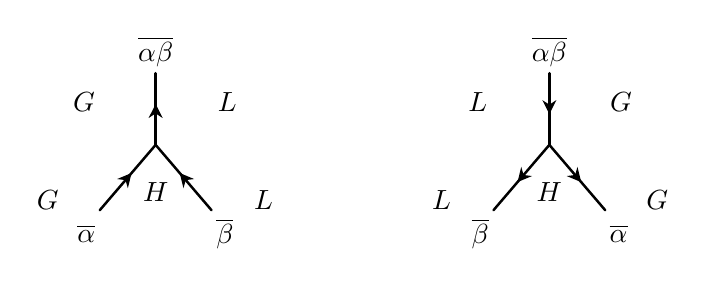
\begin{tikzpicture}[x=1cm,y=1cm]
 \draw[oriented] (-.71,-.83)--(0,0);
 \draw[oriented] (.71,-.83)--(0,0);
 \draw[oriented] (0,0)--(0,.91);
 \node at (-1.37,-.70) {$G$};
 \node at (0,-.60) {$H$};
 \node at (1.37,-.70) {$L$};
 \node at (-.91,.54) {$G$};
 \node at (.91,.54) {$L$};
 \node at (-.88,-1.13) {$\co\alpha$};
 \node at (.88,-1.13) {$\co\beta$};
 \node at (0,1.18) {$\overline{\alpha\beta}$};
 \begin{scope}[xshift=5cm]
 \draw[oriented] (0,.91)--(0,0);
 \draw[oriented] (0,0)--(-.71,-.83);
 \draw[oriented] (0,0)--(.71,-.83);
 \node at (-1.37,-.70) {$L$};
 \node at (0,-.60) {$H$};
 \node at (1.37,-.70) {$G$};
 \node at (-.91,.54) {$L$};
 \node at (.91,.54) {$G$};
 \node at (-.88,-1.13) {$\co\beta$};
 \node at (.88,-1.13) {$\co\alpha$};
 \node at (0,1.18) {$\overline{\alpha\beta}$};
 \end{scope}
\end{tikzpicture}
\end{center}

\paragraph{Diagrams and evaluated maps.}
For fixed endpoints \(K,H\), the objects of \(\mathcal D_U(K,H)\)
are sequences of strands from \(H\) to \(K\), interpreted as tensor
products. When \(K=H\), the empty sequence gives the regular bimodule.
Diagrams are built from dots, cups, caps, merges, splits, identities,
and the associativity and unit maps for tensor products, using
horizontal tensor product and vertical stacking. Each diagram has a
specified bottom source and top target. Stacking requires matching
boundary objects, including the ordered strands, orientations,
centralizer cosets, and region groups.

Fix boundary objects \(X,Y\), also writing \(X,Y\) for their
bimodules. Let \(V(X,Y)\) be the vector space of finite formal
\(\C\)-linear combinations of admissible diagrams from \(X\) to \(Y\).
For stacking we make the usual associativity and identity-wire
identifications. Evaluation is the linear map
\[
 \operatorname{ev}_{X,Y}:V(X,Y)\longrightarrow
   \Hom_{\C[K]\text{-}\C[H]}(X,Y),\qquad
 \sum_i c_i\mathsf D_i\longmapsto
   \sum_i c_i\operatorname{ev}(\mathsf D_i).
\]
A formal diagram and the bimodule map it evaluates to are distinct
objects. Different diagrams can give the same map. We identify two
linear combinations exactly when their evaluations agree, so
\[
 \Hom_{\mathcal D_U(K,H)}(X,Y)
   =V(X,Y)/\ker\operatorname{ev}_{X,Y}
   \cong\operatorname{im}\operatorname{ev}_{X,Y}.
\]
Thus each hom-space is a complex vector space of generated bimodule
maps. Representability of further bimodule maps requires a separate
argument, such as the orbit-sum construction in
Proposition~\ref{prop:orbit-hom}.

\paragraph{Composition and the diagram algebra.}
Stacking extends bilinearly:
\[
 \left(\sum_j b_j\mathsf E_j\right)\circ
 \left(\sum_i c_i\mathsf D_i\right)
   =\sum_{j,i}b_jc_i(\mathsf E_j\circ\mathsf D_i),
 \qquad \mathsf D_i:X\to Y,\quad\mathsf E_j:Y\to Z.
\]
Evaluation preserves composition. Consequently it descends to the
quotient hom-spaces, with associative composition and identity given
by the undecorated identity diagram. Horizontal tensor product of maps is
\(\mathbb C\)-bilinear; the underlying bimodules are tensored over the
group algebra of the common region.

To combine diagrams with different sources and targets in one
algebra, choose a finite family \(\mathcal X=(X_i)_{i\in F}\) of
boundary objects in \(\mathcal D_U(K,H)\), and put
\[
 A_{\mathcal X}=\bigoplus_{i,j\in F}V(X_i,X_j).
\]
An element of \(V(X_i,X_j)\) occupies block \((j,i)\). Multiply two
blocks by stacking when their intermediate boundary indices match,
and by zero otherwise; then extend bilinearly. Explicitly, for
\(\mathsf D:X_i\to X_j\) and \(\mathsf E:X_k\to X_\ell\),
\[
 \mathsf E_{\ell k}\mathsf D_{ji}=
 \begin{cases}
  (\mathsf E\circ\mathsf D)_{\ell i},&k=j,\\
  0,&k\ne j.
 \end{cases}
\]
This is associative matrix multiplication, with identity the sum of
the individual identity diagrams in the diagonal blocks.

Evaluate each block as the corresponding bimodule map on
\(\bigoplus_{i\in F}X_i\). This gives an algebra homomorphism
\(\operatorname{Ev}_{\mathcal X}\) whose kernel is the two-sided ideal
\[
 I_{\mathcal X}=\bigoplus_{i,j\in F}\ker\operatorname{ev}_{X_i,X_j}.
\]
Indeed, composing an evaluated block map with the inclusion of
\(X_i\) and the projection to \(X_j\) recovers its \((j,i)\) entry.
The quotient algebra is therefore
\[
 \mathcal A_{\mathcal X}=A_{\mathcal X}/I_{\mathcal X}
   \cong\bigoplus_{i,j\in F}
     \Hom_{\mathcal D_U(K,H)}(X_i,X_j)
   \cong\operatorname{im}\operatorname{Ev}_{\mathcal X},
\]
with multiplication as above. It is precisely the algebra of
evaluated block maps with diagrammatic entries, and is a unital
subalgebra of the bimodule endomorphisms of \(\bigoplus_iX_i\).
Every hom-space embeds as its own block. If \(e_i\) is the class of
the identity diagram in block \((i,i)\), then
\[
 1=\sum_{i\in F}e_i,\qquad
 e_i\mathcal A_{\mathcal X}e_i
   \cong\End_{\mathcal D_U(K,H)}(X_i).
\]
Thus the fixed-boundary endomorphism algebras are the diagonal
corners of the combined diagram algebra.

For an infinite family, the same construction with finite-support
block sums is locally unital: any finite collection of elements has
a common two-sided unit \(\sum_{i\in S}e_i\), where the finite set
\(S\) contains all its source and target indices. With infinitely
many nonzero boundary objects there is no global unit in this
finite-support algebra. One may adjoin a global unit by adjoining
the identity operator on \(\bigoplus_iX_i\) to its evaluated image.

In particular, for one fixed boundary object \(X\), stacking makes
\(A_X=V(X,X)\) an associative unital \(\C\)-algebra, with
\(\mathsf E\mathsf D=\mathsf E\circ\mathsf D\) read bottom to top.
Evaluation is an algebra homomorphism to the bimodule endomorphisms
of \(X\). Its kernel \(I_X\) is a two-sided ideal: for
\(n\in I_X\) and \(a,b\in A_X\),
\[
 \operatorname{ev}(anb)
   =\operatorname{ev}(a)\circ0\circ\operatorname{ev}(b)=0.
\]
The algebra of diagrammatic endomorphisms is therefore
\[
 \End_{\mathcal D_U(K,H)}(X)=A_X/I_X,
 \qquad [\mathsf E][\mathsf D]=[\mathsf E\circ\mathsf D],
 \qquad 1=[\id_X].
\]
This algebra need not be commutative. On \(\I_{\bar1}^{G,1}\), every
\(g\in G\) gives a dot \(r_g(x)=xg\), and
\(r_h\circ r_g(x)=xgh\). If \(gh\ne hg\), the two dot orders give
different maps.

\paragraph{Sums of maps and direct sums.}
Inside one hom-space, a finite linear combination may be pictured
as a superposition of diagrams with the same source and target;
evaluation adds their maps on the same input. Actual direct sums
of bimodules give different input and output summands: a direct sum
\(f\oplus g\) acts separately on those summands as a block-diagonal
map. More generally, a map
\(\bigoplus_i X_i\to\bigoplus_jY_j\) has entries
\(f_{ji}:X_i\to Y_j\), and acts by
\((x_i)_i\mapsto(\sum_i f_{ji}(x_i))_j\).
Thus sums across different boundaries in the combined algebra retain
their block positions, while superpositions add maps inside one block.
Section~\ref{sec:mackey} uses the full bimodule category for arbitrary
direct sums. Its pointwise finite infinite sums have the stated
finiteness conditions, beyond the finite combinations defining
\(V(X,Y)\).

\paragraph{Convention for diagrammatic identities.}
Throughout this article, displayed identities between diagrams are equalities
of their evaluated bimodule maps, with the same source and target.
For readability we use the slight abuse \(\mathsf D_1=\mathsf D_2\)
for \(\operatorname{ev}(\mathsf D_1)=\operatorname{ev}(\mathsf D_2)\).
The same convention applies to finite \(\C\)-linear combinations,
with evaluation extended linearly. When an indexed sum is allowed by
the stated pointwise finiteness conditions, it denotes the pointwise
sum of the evaluated maps: only finitely many terms are nonzero on
each input. Such a sum need not belong to \(V(X,Y)\), whose formal
linear combinations are finite.

\subsection{The corresponding functor category}\label{sec:functors}

Eilenberg--Watts identifies \(\C[K]\)-\(\C[H]\) bimodules with equal
scalar actions with \(\C\)-linear, right-exact, coproduct-preserving
functors from \(\C[H]\Mod\) to \(\C[K]\Mod\). Bimodule maps
correspond to natural transformations.

The category \(\mathcal D_U(K,H)\) corresponds to composites of the
given inductions and restrictions. Its transformations are built
from the indicated maps by tensor product, composition, and finite
linear combination. For a transformation between two such tensor
functors, membership is determined by its component at \(\C[H]\),
using the tensor unit identifications. Finite direct sums and
matrices of maps correspond on both sides.

These composite functors are exact and preserve coproducts.
Restriction acts on the same vector spaces, and \(\C[G]\) is free as
a right \(\C[H]\)-module along each embedding. Allowing every bimodule
map would give the full subcategory on these functors.

\Needspace{12\baselineskip}
\section{Mackey decomposition}\label{sec:mackey}

We state ordinary Mackey decomposition and give its diagrammatic
form for conjugation embeddings. Each double coset determines one
summand and its inclusion and projection.
\subsection{The ordinary Mackey theorem}

\begin{theorem}[Ordinary Mackey decomposition \cite{mackey}]\label{thm:ordinary-mackey}
Let \(K,H\le G\) be subgroups with their given inclusions. Set
\(I=K\backslash G/H\), the set of double cosets
\(KgH=\{kgh:k\in K,\ h\in H\}\) for \(g\in G\).
Choose an indexed family \((\sigma_i)_{i\in I}\) in \(G\) with
\(\sigma_i\in i\) for each \(i\). Thus \(i=K\sigma_i H\) and
\[
 G=\bigsqcup_{i\in I}K\sigma_i H .
\]
For each \(i\in I\), set \(L_i=K\cap\sigma_i H\sigma_i^{-1}\).
Use the inclusion \(L_i\hookrightarrow K\) and the embedding
\(\mu_i:L_i\hookrightarrow H\) given by \(\ell\mapsto\sigma_i^{-1}\ell\sigma_i\).
Then there is a natural isomorphism
\[
 \Res_K^G\,\Ind_H^G
    \ \cong\ \bigoplus_{i\in I}\Ind_{L_i}^K\,\Res_{\mu_i}.
\]
At the bimodule level the map from the \(i\)-th summand
\(\C[K]\otimes_{\C[L_i]}\C[H]\) to \(\C[G]\) takes
\(k\otimes h\) to \(k\sigma_i h\).
\end{theorem}

The finite-group formulation is from Khovanov
\cite[Eq.~(29) and Prop.~6]{khovanov}. The version for arbitrary groups
stated here is the case \(\alpha=\beta=1\) of Theorem~\ref{thm:mackey}.

\subsection{Generalized Mackey theorem for conjugate embeddings}
\label{sec:generalized}

Let \(K,H,G\le U\) and \(\alpha,\beta\in U\) satisfy
\(\cg{\alpha}{K}\le G\) and \(\cg{\beta}{H}\le G\).
Let \(J=(\cg{\alpha}{K})\backslash G/(\cg{\beta}{H})\). Choose one
representative \(\sigma_j\in j\) for each \(j\in J\), so
\begin{equation}\label{eq:conj-cosets}
 j=(\cg{\alpha}{K})\sigma_j(\cg{\beta}{H}),
 \qquad G=\bigsqcup_{j\in J}j.
\end{equation}
For each \(j\), set
\begin{equation}\label{eq:alt-L}
 L_j=\cg{\alpha}{K}\cap\cg{\sigma_j\beta}{H} .
\end{equation}
The embeddings out of \(L_j\) are
\(\lambda_j(\ell)=\alpha^{-1}\ell\alpha\in K\) and
\(\mu_j(\ell)=\beta^{-1}\sigma_j^{-1}\ell\sigma_j\beta\in H\).
The strand labels for these maps are
\(\overline{\alpha^{-1}}=\alpha^{-1}C_U(L_j)\) and
\(\overline{\beta^{-1}\sigma_j^{-1}}=\beta^{-1}\sigma_j^{-1}C_U(L_j)\).

Write \(M={}_{\C[K]}(\C[G])_{\C[H]}\) with actions through \(\alpha_*,\beta_*\),
and \(M_j=\C[K]\otimes_{\C[L_j]}\C[H]\) with actions in the tensor product
through \(\lambda_j,\mu_j\). A boundary with middle region \(G\)
represents \(\D_{\bar\alpha}^{K,G}\otimes_{\C[G]}\I_{\bar\beta}^{G,H}\cong M\);
one with middle region \(L_j\) represents
\(\I_{\overline{\alpha^{-1}}}^{K,L_j}\otimes_{\C[L_j]}
 \D_{\overline{\beta^{-1}\sigma_j^{-1}}}^{L_j,H}\cong M_j\).

\begin{theorem}[Generalized Mackey decomposition]\label{thm:mackey}
There are bimodule maps \(p_j:M\to M_j\) and \(\iota_j:M_j\to M\) such that
\begin{equation}\label{eq:split}
   \id_M=\sum_{j\in J}\iota_j\circ p_j,\qquad
   p_j\circ\iota_i=
   \begin{cases}
     \id_{M_i},&i=j,\\
     0,&i\ne j.
   \end{cases}
\end{equation}
The sum is pointwise finite and gives
\[
 M\cong\bigoplus_{j\in J}M_j,\qquad
 \Res_{\alpha_*}\,\Ind_{\beta_*}
   \cong\bigoplus_{j\in J}\Ind_{\lambda_j}\,\Res_{\mu_j}.
\]
\end{theorem}

The inclusion and projection diagrams below extend Khovanov's
finite-group diagrams to conjugate embeddings \cite[Prop.~6]{khovanov}.

For each \(j\), choose right coset representatives \(h_u\) indexed by
\(U_j\), so that
\begin{equation}\label{eq:H-cosets}
 H=\bigsqcup_{u\in U_j}(\cg{\beta^{-1}\sigma_j^{-1}}{L_j})h_u .
\end{equation}
For \(g\in G\), put
\[
 U'_j(g)=\{u\in U_j:
   \alpha^{-1}g\beta h_u^{-1}\beta^{-1}\sigma_j^{-1}\alpha\in K\}.
\]

\begin{lemma}[The surviving coset representative]\label{lem:first-filter}
The set \(U'_j(g)\) has exactly one element if \(g\in j\) and is
empty otherwise.
\end{lemma}

\begin{proof}
If \(u\in U'_j(g)\), then
\(g\beta h_u^{-1}\beta^{-1}\in(\cg{\alpha}{K})\sigma_j\), so \(g\in j\).
Conversely, write \(g=\alpha k\alpha^{-1}\sigma_j\beta h\beta^{-1}\)
with \(k\in K\) and \(h\in H\). Cancelling \(k\) in the defining test,
we obtain
\[
 \begin{aligned}
 u\in U'_j(g)
 &\iff \sigma_j\beta h h_u^{-1}\beta^{-1}\sigma_j^{-1}\in\cg{\alpha}{K}\\
 &\iff h h_u^{-1}\in\cg{\beta^{-1}\sigma_j^{-1}}{L_j}.
 \end{aligned}
\]
The middle expression is already in \(\cg{\sigma_j\beta}{H}\).
The last condition holds for exactly one \(u\) by \eqref{eq:H-cosets}.
\end{proof}

\begin{proof}[Proof of Theorem~\ref{thm:mackey}]
The dot \(\sigma_j\) and the multiplication cap give
\[
 \iota_j(k\otimes h)=\alpha k\alpha^{-1}\sigma_j\beta h\beta^{-1}.
\]
This formula is balanced because
\(\alpha_*(\lambda_j(\ell))=\ell\) and
\(\sigma_j\beta_*(\mu_j(\ell))=\ell\sigma_j\) for \(\ell\in L_j\).
It commutes with the left \(K\)-action and the right \(H\)-action.

For the other crossing, the reverse cup supplies the coset terms,
the dot inserts \(\sigma_j^{-1}\), and the trace
\(E_\alpha:\C[G]\to\C[K]\) keeps only the indices in \(U'_j(g)\). Thus
\[
 p_j(g)=\sum_{u\in U'_j(g)}
   \alpha^{-1}g\beta h_u^{-1}\beta^{-1}\sigma_j^{-1}\alpha\otimes h_u .
\]
Extend this formula linearly. If the coset index in \eqref{eq:H-cosets}
is infinite, apply the trace term by term. Lemma~\ref{lem:first-filter}
gives at most one term on each basis element.

\begin{center}
\begin{minipage}{.97\linewidth}
\centering
\mackeytwocrossings{G}{L_j}{G}{arrowatend}
\hspace{6mm}\(\displaystyle=\)\hspace{6mm}
\mackeyendomorphism{j}
\end{minipage}
\end{center}

Apply \(\iota_j\) to each surviving term. The dot \(\sigma_j\)
cancels \(\sigma_j^{-1}\), and \(h_u^{-1}h_u=1\), so
\begin{equation}\label{eq:first-chain}
 (\iota_j\circ p_j)(g)=|U'_j(g)|\,g .
\end{equation}
By Lemma~\ref{lem:first-filter}, this fixes \(g\) if \(g\in j\)
and sends it to zero otherwise. Each \(g\in G\) lies in exactly one
double coset. Summing over \(j\) gives \(\id_M\), and the sum is
finite on each input.

\begin{center}
\mackeyidentity{G}{\bar\alpha}{\bar\beta}{reverseoriented}{oriented}
\hspace{5mm}\(\displaystyle=\sum_{j\in J}\)\hspace{3mm}
\mackeytwocrossings{G}{L_j}{G}{arrowatend}
\end{center}

In the reverse order, let \(g=\iota_i(k\otimes h)\). Then \(g\in i\),
so \(p_j(g)=0\) for \(i\ne j\). For \(i=j\) let \(u\) be the unique
element of \(U'_j(g)\). The lemma gives
\(\ell=\sigma_j\beta h h_u^{-1}\beta^{-1}\sigma_j^{-1}\in L_j\).
Substituting into \(p_j\) and using the tensor relation gives
\begin{equation}\label{eq:second-chain}
 (p_j\circ\iota_j)(k\otimes h)
   =k\lambda_j(\ell)\otimes h_u
   =k\otimes\mu_j(\ell)h_u
   =k\otimes h .
\end{equation}

\begin{center}
\begin{minipage}{.97\linewidth}
\centering
\mackeytwocrossings{L_j}{G}{L_i}{arrowatstart}
\hspace{6mm}\(\displaystyle=\)\hspace{6mm}
\mackeyorthogonality{i}{j}
\end{minipage}
\end{center}

The two identities make \((p_j)_j\) the inverse of the bimodule map
\(\bigoplus_j M_j\to M\) with components \(\iota_j\).
Thus each \(p_j\) is a bimodule map. Tensoring the isomorphism on the
right gives the stated functor isomorphism.
\end{proof}

\Needspace{12\baselineskip}
\section{Right curls, trivalent moves, and admissible labellings}
\label{sec:curl-relations}

We establish local rules for comparing diagrams, including how
dots pass through curls or three-strand vertices, and when bending
a strand at such a vertex preserves its map.

\subsection{Right curls and dots}

The right curl on \(\I_{\bar\alpha}^{G,H}\) uses the
reverse cup and multiplication cap for the embedding by \(\delta\)
of \(K\) into \(H\). It requires \([H:\cg{\delta}{K}]<\infty\).
For the inclusion this index is \([H:K]\).

\begin{proposition}[Right curl and dot slide]\label{prop:curl}
The curl multiplies by \([H:\cg{\delta}{K}]\).
For \(d=\alpha\beta^{-1}\in G\), the dot \(r_d(x)=xd\) changes
\(\bar\alpha\) to \(\bar\beta\). Using the same embedding of \(K\)
into \(H\), the dot below, inside, or above the curl gives
\(x\mapsto[H:\cg{\delta}{K}]xd\).

For the four identities below take \(\gamma,\gamma'\) for embeddings
of \(H\) into \(G\) and \(\alpha,\beta\) for embeddings of \(K\) into \(H\).
Set \(d=\gamma(\gamma')^{-1}\in G\) and \(e=\alpha\beta^{-1}\in H\).
Write \(m_{\gamma,\alpha}\) and \(m^\downarrow_{\gamma,\alpha}\) for the
induction and restriction merges and \(\ell_a(x)=ax\).
The identities are in order for the induction merge, induction split,
restriction merge, and restriction split.
\begin{align}
 m_{\gamma',\beta}\circ(r_d\otimes r_e)
  &=r_{d\gamma'e(\gamma')^{-1}}\circ m_{\gamma,\alpha},
       \label{eq:two-leg-slide}\\
 (r_d\otimes r_e)\circ m_{\gamma,\alpha}^{-1}
  &=m_{\gamma',\beta}^{-1}\circ r_{d\gamma'e(\gamma')^{-1}},\\
 m^\downarrow_{\gamma',\beta}\circ(\ell_{e^{-1}}\otimes\ell_{d^{-1}})
  &=\ell_{\gamma'e^{-1}(\gamma')^{-1}d^{-1}}\circ
        m^\downarrow_{\gamma,\alpha},\\
 (\ell_{e^{-1}}\otimes\ell_{d^{-1}})\circ(m^\downarrow_{\gamma,\alpha})^{-1}
  &=(m^\downarrow_{\gamma',\beta})^{-1}\circ
        \ell_{\gamma'e^{-1}(\gamma')^{-1}d^{-1}} .
\end{align}
\end{proposition}

\begin{proof}[Proof of the induction merge identity]
Since \(m_{\gamma,\alpha}(x\otimes y)=x\gamma_*(y)\) and
\(d\gamma'_*(y)=\gamma_*(y)d\), we have
\[
 m_{\gamma',\beta}(xd\otimes ye)
   =xd\,\gamma'_*(ye)
   =x\gamma_*(y)\,d\gamma'_*(e).
\]
This gives \eqref{eq:two-leg-slide}.
\end{proof}


\begin{center}
\begin{minipage}{.98\linewidth}
\centering
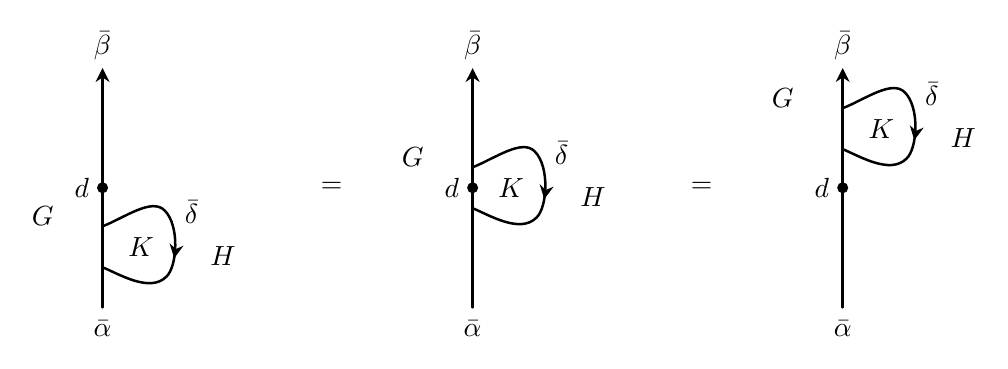
\begin{tikzpicture}[x=1cm,y=1cm,baseline=(current bounding box.center)]
 \foreach \shift/\height in {0/-.75,4.7/0,9.4/.75} {
  \begin{scope}[xshift=\shift cm]
   \draw[arrowatend] (0,-1.52)--(0,1.52);
   \draw[oriented] (0,{\height+.26})
     .. controls (.28,{\height+.37}) and (.63,{\height+.63}) .. (.79,{\height+.46})
     .. controls (.98,{\height+.27}) and (.95,{\height-.25}) .. (.81,{\height-.38})
     .. controls (.60,{\height-.59}) and (.20,{\height-.34}) .. (0,{\height-.26});
   \fill (0,0) circle (2pt);
   \node[strandlabel,anchor=east] at (-.12,0) {$d$};
   \node[strandlabel] at (0,-1.79) {$\bar\alpha$};
   \node[strandlabel] at (0,1.80) {$\bar\beta$};
   \node[region] at (-.76,{\height+.39}) {$G$};
   \node[region] at (.49,\height) {$K$};
   \node[region] at (1.53,{\height-.12}) {$H$};
   \node[strandlabel] at (1.13,{\height+.44}) {$\bar\delta$};
  \end{scope}
 }
 \node at (2.91,0) {$=$};
 \node at (7.61,0) {$=$};
\end{tikzpicture}
\end{minipage}
\end{center}

\begin{proof}[Proof of the curl identity]
Choose \(T\) with \(H=\bigsqcup_{t\in T}(\cg{\delta}{K})t\).
The cup gives \(\sum_t x\alpha_*(t^{-1})\otimes t\) in
\(\C[G]\otimes_{\C[K]}\C[H]\). The cap gives
\(\sum_t x\alpha_*(t^{-1})\alpha_*(t)=[H:\cg{\delta}{K}]x\).
A dot inside the curl inserts \(d\) in the first factor and changes
the cap to use \(\beta_*\). Since
\(\alpha_*(t^{-1})d\,\beta_*(t)=d\), the result is
\([H:\cg{\delta}{K}]xd\). This also equals composition with the
scalar curl on either side.
\end{proof}

More generally, in the full bimodule category, insert on the induction
factor the endomorphism given by right multiplication by
\(a\in\C[H]\) commuting with \(\C[\cg{\delta}{K}]\).
It is an eligible single dot under our convention when each supported
group element centralizes \(\cg{\delta}{K}\); commuting only after
addition suffices for the endomorphism in this calculation.
The resulting curl acts by right multiplication by
\[
 \alpha_*\!\left(\sum_{t\in T}t^{-1}at\right).
\]
This follows by inserting \(a\) between \(t^{-1}\) and \(t\).
Replacing \(t\) by \(\ell t\), \(\ell\in\cg{\delta}{K}\), leaves
the summand unchanged. Right multiplication permutes the cosets,
so the sum is central in \(\C[H]\). A dot between the \(\alpha_*\)
and \(\beta_*\) strands intertwines their images of this sum.

\subsection{Moving dots across a merge or split}

The diagrams below show the case \(d=1\) of the four identities in
Proposition~\ref{prop:curl}. Read from bottom to top.

\begin{center}
\tikzset{
 wire/.style={line width=.88pt,line cap=round},
 forwards/.style={wire,decoration={markings,mark=at position .23 with
      {\arrow{Stealth[length=5.4pt,width=4.8pt]}}},postaction={decorate}},
 backwards/.style={wire,decoration={markings,mark=at position .23 with
      {\arrowreversed{Stealth[length=5.4pt,width=4.8pt]}}},postaction={decorate}},
 labeltext/.style={font=\normalsize,inner sep=1.1pt}
}
\newcommand{\slidevertex}[5]{%
 \ifnum#2=1
  \def\leglabel{\bar\alpha}
  \def\mergedstrandlabel{\overline{\gamma\beta}}
  \def\innerleg{\bar\beta}
  \def\mergedstrandbelow{\overline{\gamma\alpha}}
 \else
  \def\leglabel{\bar\beta}
  \def\mergedstrandlabel{\overline{\gamma\alpha}}
  \def\innerleg{\bar\alpha}
  \def\mergedstrandbelow{\overline{\gamma\beta}}
 \fi
 \ifnum#1=1
  \def\outsideanchor{west}
  \def\insideanchor{east}
 \else
  \def\outsideanchor{east}
  \def\insideanchor{west}
 \fi
 \begin{tikzpicture}[x=1cm,y=1cm,baseline=(current bounding box.center)]
  \useasboundingbox (-2.10,-1.39) rectangle (2.10,1.39);
  \begin{scope}[xscale=#1,yscale=#2]
   \draw[#3] (-1.10,-.96) .. controls (-.74,-.66) and (-.45,-.20) .. (0,0);
   \draw[#3] (1.10,-.96) .. controls (.74,-.66) and (.45,-.20) .. (0,0)
        coordinate[pos=.48] (legdot);
   \draw[#3] (0,0)--(0,1);
   \node[labeltext] at (-1.34,.12) {$G$};
   \node[labeltext] at (1.53,.14) {$K$};
   \node[labeltext] at (0,-.77) {$H$};
   \node[labeltext] at (-1.12,-1.19) {$\bar\gamma$};
   \node[labeltext] at (1.12,-1.19) {$\leglabel$};
   \node[labeltext] at (0,1.24) {$\mergedstrandlabel$};
   \ifnum#4=0
    \fill (legdot) circle (2pt);
    \node[labeltext,anchor=\outsideanchor] at (.77,-.47) {$#5$};
    \node[labeltext,anchor=\outsideanchor] at (.36,-.18) {$\innerleg$};
   \else
    \fill (0,.60) circle (2pt);
    \node[labeltext,anchor=\outsideanchor] at (.15,.62) {$#5$};
    \node[labeltext,anchor=\insideanchor] at (-.13,.28) {$\mergedstrandbelow$};
   \fi
  \end{scope}
 \end{tikzpicture}%
}
\newcommand{\slideequation}[4]{%
 \slidevertex{#1}{#2}{#3}{0}{#4}\enspace
 \(=\)\enspace
 \slidevertex{#1}{#2}{#3}{1}{\gamma#4\gamma^{-1}}%
}
\begin{minipage}{.98\linewidth}
 \centering
 \textbf{Induction merge}\par
 \slideequation{1}{1}{forwards}{e}\par\smallskip
 \textbf{Induction split}\par
 \slideequation{1}{-1}{backwards}{e}
\end{minipage}\par\smallskip
\begin{minipage}{.98\linewidth}
 \centering
 \textbf{Restriction merge}\par
 \slideequation{-1}{1}{backwards}{e^{-1}}\par\smallskip
 \textbf{Restriction split}\par
 \slideequation{-1}{-1}{forwards}{e^{-1}}
\end{minipage}
\end{center}

\paragraph{Moving a dot back to a branch.}
Fix the incoming labels of a merge. A dot \(D\in G\) on its merged
strand can move to the right input exactly when \(D\in\cg{\gamma}{H}\).
Necessity follows from \eqref{eq:two-leg-slide} with \(d=1\).
For sufficiency take \(e=\gamma^{-1}D\gamma\in H\) and
\(\beta=e^{-1}\alpha\). This embeds \(K\) into \(H\) and gives the
same output embedding, since both conjugate \((\gamma\alpha)_*\)
by \(D^{-1}\). A dot can always move to the left input by taking
\(\gamma'=D^{-1}\gamma\) and \(e=1\).

For a split with left label \(\bar\alpha\), moving a dot to the
right output requires \(D\in\cg{\alpha}{H}\). To move it to the
left output, factor the given input representative \(b\) as
\((b\gamma^{-1})\gamma\). Since
\(D=b(\alpha\gamma)^{-1}\), the left representative
\(b\gamma^{-1}=D\alpha\) embeds \(H\) into \(G\).

\paragraph{Moving a curl across a vertex.}
A right curl with no dot multiplies by its index. It can move
across a merge or split if the new curl has the same index.
The right input and the merged strand have the same right
region \(K\). The left input has right region \(H\), where
\[
 [H:\cg{\alpha}{L}]=[H:\cg{\alpha}{K}]\,[K:L]
\]
for \(L\le K\) and finite indices.

\begin{example}[Two curls with different indices]\label{ex:different-curl-indices}
For \(G=H=C_2\) and \(K=L=1\),
the curls using \(1\) multiply by \(1\) on the right input and
by \(2\) on the left.
\end{example}

Dividing each curl by its finite index
gives the identity.

\subsection{When one shape can replace another}

For shapes \(A,B\) with the same boundary shape, write \(A\preceq B\)
if every labelling of \(A\) can be replaced by a labelling of \(B\)
with the same boundary groups, boundary cosets, and map. Internal
labels may change. This is inclusion of the sets of maps at each
fixed boundary, so the relation is reflexive and transitive.

\Needspace{6\baselineskip}
\begin{proposition}\label{prop:preorder-not-symmetric}
Let \(A\) be the induction merge with a dot on the right input, and
let \(B\) be the induction merge with a dot on the merged strand. Then
\(A\preceq B\) and \(B\npreceq A\).
\end{proposition}
\begin{proof}
The induction-merge slide in \eqref{eq:two-leg-slide} is defined for
every admissible labelling of \(A\) and preserves its boundary and map.


Example~\ref{ex:dot-slide-obstruction} proves \(B\npreceq A\).
\end{proof}

\begin{example}[A dot that cannot move to the right input]\label{ex:dot-slide-obstruction}
Take the standard inclusions in the finitary symmetric group
\[
   K=\operatorname{Sym}(\{1,2\})\ \le\
   H=\operatorname{Sym}(\{1,2,3\})\ \le\
   G=\operatorname{Sym}(\{1,2,3,4\}).
\]
Fix all boundary strands to be these inclusions and their composite.
Put \(g=(3\,4)\) on the merged strand of \(B\). It centralizes
\(K\), so \(g,1\) represent the same label there. The map sends
\(1\otimes1\) to \(g\). In shape \(A\), the image of \(1\otimes1\)
is the right-input label and lies in \(H\), whereas \(g\notin H\).
\end{example}


\subsection{Maps between induction bimodules}

\begin{proposition}\label{prop:orbit-hom}
The space of bimodule maps from \(\I_{\bar\alpha}^{G,H}\) to
\(\I_{\bar\beta}^{G,H}\) has a basis given by right multiplication
by the sums of the finite orbits of
\[
       h\cdot g=\alpha_*(h)g\,\beta_*(h)^{-1}
       \qquad(h\in H,\ g\in G).
\]
The single group-element dots are the singleton orbits. If \(H\) is
finite, the sum over each orbit is realized by a diagram.
\end{proposition}
\begin{proof}
A left \(\C[G]\)-linear map is right multiplication by its value \(a\)
at \(1\). It respects the \(\C[H]\)-action precisely when
\(\alpha_*(h)a=a\beta_*(h)\) for every \(h\). Invariance forces the
coefficients to be constant on an orbit, and finite support excludes
infinite orbits. This proves the basis statement.

For finite \(H\), insert the reverse cup for \(1\hookrightarrow H\)
on the right of the \(\bar\alpha\)-strand. Merge the two induction
strands to an induction from \(1\) to \(G\), put the dot \(g\) on
that strand, then split using the \(\bar\beta\)-strand and apply the
multiplication cap for \(1\hookrightarrow H\). The resulting value
at \(x\) is
\[
 x\sum_{t\in H}\alpha_*(t^{-1})g\beta_*(t)
   =x\,|\operatorname{Stab}_H(g)|\sum_{z\in H\cdot g}z .
\]
The stabilizer order is invertible in \(\C\).
\end{proof}


\begin{example}[A block swap]\label{ex:block-swap}
Let
\[
 B_1=\{1,2,3\},\quad B_2=\{4,5,6\},\quad
 B_3=\{7,8,9\},\quad B_4=\{10,11,12\}.
\]
Put
\[
 G=\operatorname{Sym}(B_1\cup B_2)\times\operatorname{Sym}(B_3\cup B_4),
 \qquad H=\prod_{i=1}^4\operatorname{Sym}(B_i).
\]
Take \(\alpha=(4\,7)(5\,8)(6\,9)\) and \(\beta=1\).
The embeddings send \((4\,5)\) to transpositions in different
\(G\)-blocks. Every element of \(G\) preserves the two blocks,
so there is no group-element dot between these embeddings.
The sum over the orbit of \(1\) gives a nonzero diagram map by
Proposition~\ref{prop:orbit-hom}.
\end{example}

\paragraph{A criterion for group-element dots.}
Suppose \(H,G\) are products of symmetric groups on disjoint
blocks in the group of finitely supported permutations. Each
embedding sends a non-singleton \(H\)-block into a \(G\)-block.
A dot exists exactly when the two images of each non-singleton
\(H\)-block lie in the same \(G\)-block. Necessity follows by
testing transpositions. For sufficiency extend
\(\beta(x)\mapsto\alpha(x)\) on those images to permutations in
the \(G\)-blocks. These partial bijections differ from the
identity at finitely many points, so the extensions can have
finite support. Together they give a dot in \(G\).


\begin{example}[A dot between two images in one block]\label{ex:dot-in-one-block}
\(1\) and \((2\,3)\) send \(\{1,2\}\) to different
sets in \(S_4\), and \((2\,3)\) gives a dot.
\end{example}

\paragraph{A stronger embedding condition.}
Fix a representative \(\beta\) for the embedding of \(K\) into \(H\).
Suppose \(\cg{\sigma\beta^{-1}}{H}\le G\) whenever
\(\cg{\sigma}{K}\le G\). A reverse slide onto the right leg
can still fail.

\begin{example}[A reverse slide under the stronger embedding condition]\label{ex:stronger-slide-obstruction}
Use
\(K=\prod_i\operatorname{Sym}(B_i)\),
\(H=\operatorname{Sym}(B_1\cup B_2)\times\operatorname{Sym}(B_3\cup B_4)\),
\(G=S_{\{1,\ldots,12\}}\), and \(\beta=1\). If
\(\cg{\sigma}{K}\le G\), the support of \(\cg{\sigma}{K}\) forces
\(\sigma\) to preserve \(\{1,\ldots,12\}\), so
\(\cg{\sigma}{H}\le G\). The block swap \(\alpha=(4\,7)(5\,8)(6\,9)\)
conjugates \(K\) to itself and lies in \(G\setminus H\).
It labels a dot on the merged strand from the inclusion to
\(\bar\alpha\). It cannot move to the right input because it lies
outside \(H\).
\end{example}

\paragraph{Bounds on the support of representatives.}
For a finite subgroup \(X\) given by symmetric groups on disjoint
blocks, let \(\operatorname{supp}X\) be the union of its non-singleton blocks
and \(\widehat X=\operatorname{Sym}(\operatorname{supp}X)\). The conditions
\(\alpha\in G\widehat H\) and \(\beta\in H\widehat K\) do not ensure
\(\alpha\beta\in G\widehat K\).


\begin{example}[Support bounds under composition]\label{ex:support-composite}
Take
\[
 G=H=\operatorname{Sym}(\{1,\ldots,6\})
         \times\operatorname{Sym}(\{7,\ldots,12\}),
 \qquad K=\operatorname{Sym}(\{1,2,3\}).
\]
Let \(\alpha\) swap the two six-point blocks and let \(\beta=1\).
The two embeddings satisfy the support bounds.
Every element of \(G\widehat K\) preserves each six-point block,
whereas \(\alpha\beta\) carries the support of \(K\) into the second
block. Even the composite strand label has no representative
in \(G\widehat K\).
\end{example}


\begin{example}[Support bounds for an inverse product]\label{ex:support-inverse-product}
Consider whether \(\cg{\beta\alpha^{-1}}{H}\le G\)
when \(\alpha,\beta\in\widehat G H\) both embed \(H\) in \(G\). Take \(G\) to be the product of the symmetric groups on
\(\{1,2\},\{3,4\},\{5,6\}\), \(H=\operatorname{Sym}(\{1,2\})\),
\(\alpha=(1\,3)(2\,4)\), and \(\beta=(4\,5)\).
Both permutations belong to \(\widehat G H\) and embed \(H\) in \(G\).
But \(\beta\alpha^{-1}\) sends \(\{1,2\}\) to \(\{3,5\}\), so
\(\cg{\beta\alpha^{-1}}{H}\nleq G\).
\end{example}


\Needspace{19\baselineskip}
\subsection{Bends at a trivalent vertex}
\begin{proposition}[Bend identities]\label{prop:trivalent-bends}
Let \(K\xrightarrow{\alpha_*}H\xrightarrow{\gamma_*}G\)
be conjugation embeddings. The two diagrams in each pair below
give the same bimodule map. The multiplication-cap and ordinary-cup
identities hold at all indices. The trace-cap identity holds when
\([H:\cg{\alpha}{K}]<\infty\), and the reverse-cup identity holds when
\([G:\cg{\gamma\alpha}{K}]<\infty\).
\end{proposition}

\begingroup
\newcommand{\bendfigure}[9]{%
 \begin{tikzpicture}[x=1.13cm,y=1.07cm,baseline=(current bounding box.center)]
  \useasboundingbox (-2.05,-1.52) rectangle (2.48,1.52);
  \begin{scope}[xscale=#2,yscale=#3]
   \ifnum#1=0
    % The left branch continues into the arc and the external strand.
    \draw[#4] (-1.20,-1.02)
       .. controls (-1.02,-.61) and (-.74,-.42) .. (-.62,-.26);
    \draw[#4] (-.62,-.26)
       .. controls (-.52,.02) and (-.62,.62) .. (-.56,1.06);
    \draw[wire] (-.62,-.26)
       .. controls (-.44,-.04) and (-.13,.46) .. (.18,.47);
    \draw[#4] (.18,.47)
       .. controls (.55,.46) and (1.11,-.49) .. (1.22,-1.02);
    \node at (-.57,1.29) {$#8$};
    \node at (.43,.69) {$#9$};
   \else
    % The right branch meets the cap and turns through the smaller bend.
    \draw[#4] (-1.20,-1.02)
       .. controls (-1.04,-.54) and (-.53,.47) .. (0,.47);
    \draw[wire] (0,.47)
       .. controls (.25,.47) and (.48,.17) .. (.65,-.08);
    \draw[#4] (.65,-.08)
       .. controls (.84,-.35) and (1.10,-.72) .. (1.22,-1.02);
    \draw[wire] (.65,-.08)
       .. controls (.87,-.33) and (1.18,-.43) .. (1.36,-.36);
    \draw[#4] (1.36,-.36)
       .. controls (1.64,-.30) and (1.49,.64) .. (1.68,1.06);
    \node at (1.68,1.29) {$#8$};
    \node at (.21,.69) {$\overline{\gamma\alpha}$};
    \node at (1.12,-.02) {$#8$};
   \fi
   \node at (-1.67,.15) {$#5$};
   \node at (0,-.68) {$#6$};
   \node at (2.02,.10) {$#7$};
   \node at (-1.20,-1.27) {$\overline{\gamma\alpha}$};
   \node at (1.22,-1.26) {$#9$};
  \end{scope}
 \end{tikzpicture}%
}
\newcommand{\bendrow}[9]{%
 {\bfseries #1}\par
 \bendfigure{0}{#2}{#3}{#4}{#5}{#6}{#7}{#8}{#9}
 \hspace{4mm}\(=\)\hspace{4mm}
 \bendfigure{1}{#2}{#3}{#4}{#5}{#6}{#7}{#8}{#9}\par
}
\begin{center}
\begin{minipage}{.98\linewidth}
\centering
\bendrow{Multiplication cap}{1}{1}{oriented}{G}{K}{H}{\bar\gamma}{\bar\alpha}
\smallskip
\bendrow{Trace cap}{1}{1}{reverseoriented}{K}{G}{H}{\bar\alpha}{\bar\gamma}
\end{minipage}
\end{center}

\begin{center}
\begin{minipage}{.98\linewidth}
\centering
\bendrow{Ordinary cup}{-1}{-1}{reverseoriented}{K}{G}{H}{\bar\alpha}{\bar\gamma}
\smallskip
\bendrow{Reverse cup}{1}{-1}{reverseoriented}{G}{K}{H}{\bar\gamma}{\bar\alpha}
\end{minipage}
\end{center}
\endgroup

\begin{proof}
Read the diagrams from bottom to top and evaluate on group elements.
Use the merges, splits, and trace caps \(E_\delta\) of
Section~\ref{sec:diagram-category}.

\textbf{Multiplication cap.}
For \(g\otimes h\in\C[G]\otimes_{\C[K]}\C[H]\), we obtain
\[
\begin{aligned}
\text{LHS}\quad g\otimes h
 &\longmapsto g\otimes1\otimes h
 \longmapsto g\otimes h
 \longmapsto g\gamma_*(h),\\
\text{RHS}\quad g\otimes h
 &\longmapsto g\otimes h\otimes1\otimes1
 \longmapsto g\otimes\gamma_*(h)\otimes1
 \longmapsto g\gamma_*(h).
\end{aligned}
\]
The left cap multiplies in \(H\), then balancing over \(\C[H]\)
identifies \(g\otimes h\) with \(g\gamma_*(h)\). On the right, the
ordinary cup inserts \(1\otimes1\), and the cap multiplies in \(G\).

\textbf{Trace cap.}
Choose \(h_i\in H\) with
\(H=\bigsqcup_{i\in I}(\alpha K\alpha^{-1})h_i\).
On \(g\otimes g'\in\C[G]\otimes_{\C[G]}\C[G]\), the left side is
\[
\text{LHS}\quad g\otimes g'
 \longmapsto 1\otimes g\otimes g'
 \longmapsto 1\otimes E_\gamma(gg')
 \longmapsto E_\gamma(gg').
\]
The reverse cup on the right inserts \(\sum_i h_i^{-1}\otimes h_i\).
\[
\begin{aligned}
\text{RHS}\quad g\otimes g'
 &\longmapsto \sum_i g\otimes g'\otimes h_i^{-1}\otimes h_i\\
 &\longmapsto \sum_i g\otimes g'\gamma_*(h_i^{-1})\otimes h_i\\
 &\longmapsto \sum_i
    \alpha_*\!\left(E_{\gamma\alpha}
        (gg'\gamma_*(h_i^{-1}))\right)h_i.
\end{aligned}
\]
If \(gg'\notin\gamma H\gamma^{-1}\), all terms vanish. If
\(gg'=\gamma_*(h)\), only the \(i\) with
\(hh_i^{-1}\in\alpha K\alpha^{-1}\) survives. Its term is
\((hh_i^{-1})h_i=h=E_\gamma(gg')\).

\textbf{Ordinary cup.}
For \(h\in\C[H]\), the two outputs are
\[
\begin{aligned}
\text{LHS}\quad h
 &\longmapsto 1\otimes1\otimes h
 \longmapsto 1\otimes\gamma_*(h),\\
\text{RHS}\quad h
 &\longmapsto h\otimes1\otimes1
 \longmapsto \gamma_*(h)\otimes1.
\end{aligned}
\]
They are equal by balancing over \(\C[G]\).

\textbf{Reverse cup.}
Use the same \(h_i\) as in the trace cap. On the left,
\[
\text{LHS}\quad g
 \longmapsto \sum_i g\otimes h_i^{-1}\otimes h_i
 \longmapsto \sum_i g\gamma_*(h_i^{-1})\otimes h_i.
\]
Choose \(g_j\) with \(G=\bigsqcup_j(\gamma H\gamma^{-1})g_j\) and
\(g_0=1\). Then \(\gamma_*(h_i)g_j\) are representatives for
the cosets \(((\gamma\alpha)K(\gamma\alpha)^{-1})\gamma_*(h_i)g_j\).
On the right, write the input as \(g\otimes1\) over \(\C[G]\)
before applying the large cup. The cup, split, and trace give
\[
\begin{aligned}
\text{RHS}\quad g
 &\longmapsto \sum_{i,j}
     g(\gamma_*(h_i)g_j)^{-1}\otimes\gamma_*(h_i)g_j\otimes1\\
 &\longmapsto \sum_{i,j}
     g(\gamma_*(h_i)g_j)^{-1}\otimes1\otimes\gamma_*(h_i)g_j\otimes1\\
 &\longmapsto \sum_{i,j}
     g(\gamma_*(h_i)g_j)^{-1}\otimes E_\gamma(\gamma_*(h_i)g_j)\\
 &=\sum_i g\gamma_*(h_i^{-1})\otimes h_i.
\end{aligned}
\]
Only \(j=0\) survives the trace. The finite index for the large cup
also makes the smaller cup on the left finite.
\end{proof}

\Needspace{5\baselineskip}
The equations let us draw the vertices with three straight segments.

\begin{center}
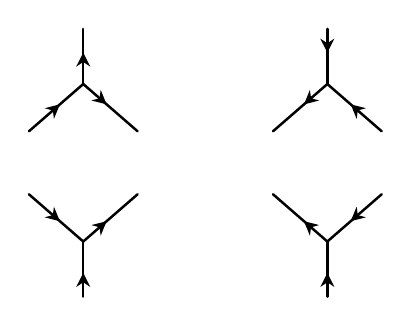
\begin{tikzpicture}[x=1cm,y=1cm]
 \foreach \col/\row/\flip/\leftarm/\rightarm/\mergedarm in {
    0/0/1/oriented/reverseoriented/oriented,
    3.1/0/1/reverseoriented/oriented/reverseoriented,
    0/-2.0/-1/oriented/reverseoriented/reverseoriented,
    3.1/-2.0/-1/reverseoriented/oriented/reverseoriented} {
   \begin{scope}[shift={(\col,\row)},yscale=\flip]
    \draw[\leftarm] (-.69,-.60)--(0,0);
    \draw[\rightarm] (.69,-.60)--(0,0);
    \draw[\mergedarm] (0,0)--(0,.70);
   \end{scope}
 }
\end{tikzpicture}
\end{center}

\Needspace{12\baselineskip}
\section{Reidemeister I move}\label{sec:reidemeister-one}

We evaluate each of the four oriented curls and identify the two
that multiply the identity by a subgroup index.

Use \(K\xrightarrow{\delta_*}H\xrightarrow{\alpha_*}G\).
The subscript on \(\id\) lists the groups on the left and right.

\Needspace{7\baselineskip}
\begin{theorem}[Reidemeister I]\label{thm:reidemeister-one}
The four curls shown below satisfy
\begin{align}
 \text{right curl on an up-strand}   &=
       [H:\cg{\delta}{K}]\,\id_{G\cdot H}, \label{eq:curl-right-up}\\
 \text{right curl on a down-strand} &=
       \id_{K\cdot H}, \label{eq:curl-right-down}\\
 \text{left curl on an up-strand}    &=
       \id_{H\cdot K}, \label{eq:curl-left-up}\\
 \text{left curl on a down-strand}   &=
       [H:\cg{\delta}{K}]\,\id_{H\cdot G}. \label{eq:curl-left-down}
\end{align}
The \(K\)-loops require finite \([H:\cg{\delta}{K}]\).
The \(G\)-loops hold at arbitrary index.
\end{theorem}

\begin{center}
\begin{minipage}{.97\linewidth}
\centering
\newcommand{\reidemeistercurl}[8]{%
 \begin{tikzpicture}[x=1cm,y=1cm,baseline=-.61cm]
   \useasboundingbox (-2.13,-1.07) rectangle (2.13,.85);
   \draw[#2] (0,-.76)--(0,.76);
   \begin{scope}[xscale=#1]
     \draw[#3] (0,.27)
       .. controls (.34,.36) and (.71,.62) .. (.95,.45)
       .. controls (1.20,.27) and (1.17,-.24) .. (.98,-.42)
       .. controls (.71,-.67) and (.30,-.36) .. (0,-.27);
     \node[region] at (.55,0) {$#6$};
     \node[strandlabel] at (1.24,-.58) {$#8$};
   \end{scope}
   \node[region] at (-1.80,0) {$#4$};
   \node[region] at (1.80,0) {$#5$};
   \node[strandlabel] at (0,-.96) {$#7$};
 \end{tikzpicture}%
}
\begin{tabular}{@{}c@{\hspace{13mm}}c@{}}
 \reidemeistercurl{1}{arrowatend}{oriented}{G}{H}{K}{\bar\alpha}{\bar\delta}
 &
 \reidemeistercurl{1}{arrowatstart}{reverseoriented}{K}{H}{G}{\bar\delta}{\bar\alpha}
 \\
 Right curl, up & Right curl, down \\[.65ex]
 \reidemeistercurl{-1}{arrowatend}{oriented}{H}{K}{G}{\bar\delta}{\bar\alpha}
 &
 \reidemeistercurl{-1}{arrowatstart}{reverseoriented}{H}{G}{K}{\bar\alpha}{\bar\delta}
 \\
 Left curl, up & Left curl, down
\end{tabular}
\end{minipage}
\end{center}

\Needspace{26\baselineskip}
\begin{proof}
For the loops enclosing \(K\), choose \(T\subseteq H\) with
\(H=\bigsqcup_{t\in T}(\cg{\delta}{K})t\). The reverse cup inserts
\(\sum_t t^{-1}\otimes t\). Apply \(\alpha_*\) to each factor
before multiplying.
\[
\begin{aligned}
 \text{right curl, up}\quad &x\longmapsto
   \sum\nolimits_{t\in T}x\,\alpha_*(t^{-1})\alpha_*(t)
   =[H:\cg{\delta}{K}]\,x,\\
 \text{left curl, down}\quad &x\longmapsto
   \sum\nolimits_{t\in T}\alpha_*(t^{-1})\alpha_*(t)\,x
   =[H:\cg{\delta}{K}]\,x .
\end{aligned}
\]

For the loops enclosing \(G\), the ordinary unit inserts
\(1\otimes1\). The join uses the composite embedding, and the
cap applies \(E_\alpha\) to the product.
\[
\begin{aligned}
 \text{right curl, down}\quad &x\longmapsto
   \alpha_*(x)\otimes1\longmapsto E_\alpha(\alpha_*(x))=x,\\
 \text{left curl, up}\quad &x\longmapsto
   1\otimes\alpha_*(x)\longmapsto E_\alpha(\alpha_*(x))=x .
\end{aligned}
\]
Here \(E_\alpha\alpha_*=\id_{\C[H]}\). Tensoring gives the functor
identities.
\end{proof}

Over \(\C\), dividing either \(K\)-loop by its finite index
\([H:\cg{\delta}{K}]\) gives the identity.


\Needspace{12\baselineskip}
\section{Reidemeister II move}\label{sec:reidemeister-two}

We evaluate pairs of crossings. For strands pointing in opposite
directions, the identities come from Mackey decomposition. For
parallel strands, merging reduces the composite to multiplication
by a single element of the group algebra.

\subsection{Mixed orientations and Mackey decomposition}
Use \(J,\sigma_j,L_j,M,M_j\) from Section~\ref{sec:generalized}.
The two boundary strands of \(M\) point in opposite directions,
with \(G\) between them. To allow a different middle group, take
\(\cg{a}{L}\le K\), \(\cg{b}{L}\le H\) and
\(s=\alpha a(\beta b)^{-1}\in G\). Use \(s,s^{-1}\) as the two
crossing labels and put
\[
 M_L=\C[K]\otimes_{\C[L]}\C[H],\qquad
 L_s=(\cg{\alpha}{K})\cap(\cg{s\beta}{H}),\qquad
 n=[L_s:\cg{\alpha a}{L}].
\]
The tensor product has basis \(K\times_L H\), the classes \([k,h]\)
of pairs under \([ka\ell a^{-1},h]=[k,b\ell b^{-1}h]\),
\(\ell\in L\). The relation identifies exactly the pairs equated
by balancing the tensor product.

\begin{proposition}[Two crossings with opposite orientations]\label{prop:r2-mixed-composition}
Suppose \(n<\infty\). Let \(p_L:M\to M_L\) and \(\iota_L:M_L\to M\)
be the two crossings. Write
\(q([k,h])=\alpha k\alpha^{-1}s\beta h\beta^{-1}\).
If \(s\in j\), then
\[
 \iota_L\circ p_L=nP_j,\qquad
 p_L\circ\iota_L(z)=\sum_{q(w)=q(z)}w \quad(z\in K\times_L H),
\]
where \(P_j\) fixes the basis elements in \(j\) and sends the others
to zero. The second composite is the identity exactly when \(n=1\).
For \(n>1\), no scalar multiple of it is the identity.
\end{proposition}

\begin{proof}
Since \(s\beta b=\alpha a\), conjugation by \(s\) identifies the
two images of \(L\). Thus \(\cg{\alpha a}{L}\le L_s\) and \(q\)
respects the relation on pairs. The dot \(s\) and multiplication
cap give \(\iota_L([k,h])=q([k,h])\).

Choose \(T\) with \(H=\bigsqcup_{t\in T}(\cg{b}{L})t\).
The reverse cup supplies \(t^{-1}\otimes t\), the dot multiplies
the first factor by \(s^{-1}\), and the trace \(E_\alpha\) gives
\[
 p_L(g)=\sum_{t\in T}
 E_\alpha\bigl(g\beta t^{-1}\beta^{-1}s^{-1}\bigr)\otimes t .
\]
Each class has a unique representative \((k,t)\) with \(t\in T\).
The trace returns \(k\) exactly when \(q([k,t])=g\).
Hence \(p_L(g)=\sum_{q(w)=g}w\).

The action of \(K\times H\) is
\((k_0,h_0)[k,h]=[k_0k,hh_0^{-1}]\) and
\((k_0,h_0)g=\alpha k_0\alpha^{-1}g\beta h_0^{-1}\beta^{-1}\).
The balanced set is transitive and \(q\) is equivariant with image
\(j\). Sending \((k_0,h_0)\) to \(\alpha k_0\alpha^{-1}\)
identifies the stabilizers of \(s\) and \([1,1]\) with \(L_s\)
and \(\cg{\alpha a}{L}\), respectively. Their index gives \(n\)
preimages for each \(g\in j\). The sums are therefore finite
and define a bimodule map. Applying \(q\) to the sum gives \(ng\)
on \(j\). In the other order the result sums all preimages of
\(q(z)\). If \(n>1\), this includes a basis element besides \(z\).
\end{proof}

The reverse cup is a map when \([H:\cg{b}{L}]<\infty\). At infinite
index the formula for \(p_L\) sums only the terms that survive the trace.
It still defines a map for finite \(n\). For infinite \(n\), the sum
on \(g\in j\) has infinite support.

\paragraph{Mackey cancellation.}
Take \(L=L_j\), \(a=\alpha^{-1}\), \(b=\beta^{-1}\sigma_j^{-1}\).
Then \(s=\sigma_j\), \(n=1\), and the two orders give
\[
 p_j\circ\iota_i=
 \begin{cases}
   \id_{M_i},&i=j,\\
   0,&i\ne j,
 \end{cases}
 \qquad
 \sum_{j\in J}\iota_j\circ p_j=\id_M .
\]
Here \(q\) is a bijection onto \(j\).
For \(i\ne j\), \(p_j\) vanishes on the image of \(\iota_i\).
The projections sum to the identity because the double cosets
partition \(G\). Read the diagrams from bottom to top.

\newcommand{\rTwoMixedCrossings}[7]{%
 \begin{tikzpicture}[baseline=(current bounding box.center),x=1cm,y=1cm]
  \draw[#3] (.72,-1.22)
    .. controls (.72,-.94) and (.34,-.79) .. (0,-.61)
    .. controls (-.35,-.42) and (-.72,-.22) .. (-.72,0)
    .. controls (-.72,.22) and (-.35,.42) .. (0,.61)
    .. controls (.34,.79) and (.72,.94) .. (.72,1.22);
  \draw[#3] (-.72,1.22)
    .. controls (-.72,.94) and (-.34,.79) .. (0,.61)
    .. controls (.35,.42) and (.72,.22) .. (.72,0)
    .. controls (.72,-.22) and (.35,-.42) .. (0,-.61)
    .. controls (-.34,-.79) and (-.72,-.94) .. (-.72,-1.22);
  \node[region] at (0,1.04) {$#1$};
  \node[region] at (0,0) {$#2$};
  \node[region] at (0,-1.04) {$#1$};
  \node[region] at (-1.11,0) {$K$};
  \node[region] at (1.11,0) {$H$};
  \node[strandlabel,anchor=west] at (.36,-.61) {$#4$};
  \node[strandlabel,anchor=west] at (.36,.61) {$#5$};
  \node[strandlabel] at (-.72,1.47) {$#6$};
  \node[strandlabel] at (.72,1.47) {$#7$};
  \node[strandlabel] at (-.72,-1.47) {$#6$};
  \node[strandlabel] at (.72,-1.47) {$#7$};
 \end{tikzpicture}%
}
\begin{center}
\begin{tabular}{@{}c@{\hspace{3mm}}c@{\hspace{3mm}}c@{\hspace{10mm}}c@{\hspace{3mm}}c@{\hspace{3mm}}c@{}}
 \rTwoMixedCrossings{L_j}{G}{arrowatstart}{\iota_j}{p_j}
    {\overline{\alpha^{-1}}}{\overline{\beta^{-1}\sigma_j^{-1}}}
 & \(=\) &
 \mackeyidentity{L_j}{\overline{\alpha^{-1}}}
   {\overline{\beta^{-1}\sigma_j^{-1}}}{arrowatend}{arrowatstart}
 &
 \(\displaystyle\sum_{j\in J}\)\,
 \rTwoMixedCrossings{G}{L_j}{arrowatend}{p_j}{\iota_j}{\bar\alpha}{\bar\beta}
 & \(=\) &
 \mackeyidentity{G}{\bar\alpha}{\bar\beta}{arrowatstart}{arrowatend}
\end{tabular}
\end{center}

\Needspace{8\baselineskip}
\begin{lemma}[Transport to the Mackey representative]\label{lem:mackey-transport}
Let \(s=\alpha a(\beta b)^{-1}\in j\) and write
\[
 s=(\alpha k\alpha^{-1})\sigma_j(\beta h\beta^{-1}),
 \qquad k\in K,\quad h\in H.
\]
Then \(L'=\cg{\alpha k^{-1}a}{L}\le L_j\). Use the restrictions of
\(\lambda_j,\mu_j\) for the embeddings of \(L'\). The map
\[
 [x,y]_L\longmapsto[xk,hy]_{L'}
\]
is a bijection respecting the left \(K\)-action and right \(H\)-action.
Its linear extension intertwines the multiplication crossings with
labels \(s,\sigma_j\), and the projection crossings with labels
\(s^{-1},\sigma_j^{-1}\) when their fiber sums are finite.
Moreover, \([L_j:L']=[L_s:\cg{\alpha a}{L}]\).
\end{lemma}

\begin{proof}
Multiplying the factorization of \(s\) by \(\beta b\) gives
\(t=\alpha k^{-1}a=\sigma_j\beta hb\). The first expression puts
\(tLt^{-1}\) inside \(\cg{\alpha}{K}\) and the second puts it inside
\(\cg{\sigma_j\beta}{H}\). Hence \(L'=tLt^{-1}\le L_j\).
For \(\ell\in L\) the restricted embeddings send \(t\ell t^{-1}\) to
\[
 \lambda_j(t\ell t^{-1})=k^{-1}a\ell a^{-1}k,\qquad
 \mu_j(t\ell t^{-1})=hb\ell b^{-1}h^{-1}.
\]
These identities carry the balancing relation for \(L\) to the one
for \(L'\) and back under the inverse shifts. The shifts commute with
the left \(K\)-action and right \(H\)-action. The crossing values agree
by
\[
 \alpha(xk)\alpha^{-1}\sigma_j\beta(hy)\beta^{-1}
 =\alpha x\alpha^{-1}s\beta y\beta^{-1}.
\]
The bijection also identifies the fibers, so it intertwines the
reverse crossings when the fiber sums are finite.
Finally, conjugation by \(\alpha k^{-1}\alpha^{-1}\) takes \(L_s\)
to \(L_j\) and \(\cg{\alpha a}{L}\) to \(L'\), proving the index equality.
\end{proof}

This justifies restricting the Mackey embeddings in the calculation
below. For any admissible dot in \(j\), the composite on \(\C[G]\)
is the projection onto \(j\) multiplied by the transported index,
whenever the reverse crossing is defined.


\paragraph{Smaller internal groups and intersections.}
Restrict the embeddings of \(L_j\) to \(L\le L_j\), and write
\(p_{L,j},\iota_{L,j}\) for the resulting crossings. For finite
\([L_j:L]\), Proposition~\ref{prop:r2-mixed-composition} gives
\(\iota_{L,j}\circ p_{L,j}=[L_j:L]\,(\iota_j\circ p_j)\).

In the rightmost diagram, \(q\) maps balanced pairs to the double coset \(j\).
\[
 q:K\times_L H\longrightarrow j,\qquad
 q([k,h]_L)=\alpha k\alpha^{-1}\sigma_j\beta h\beta^{-1}.
\]
The lower crossing \(\iota_{L,j}\) is the linear extension of \(q\).
The upper crossing \(p_{L,j}\) sends \(q(z)\) to the sum of its
\([L_j:L]\) preimages, so \(p_{L,j}\circ\iota_{L,j}\) is the
identity exactly when \(L=L_j\).

\begin{center}
 \rTwoMixedCrossings{G}{L}{arrowatend}{p_{L,j}}{\iota_{L,j}}{\bar\alpha}{\bar\beta}
 \hspace{2mm}\(=[L_j:L]\)\hspace{2mm}
 \rTwoMixedCrossings{G}{L_j}{arrowatend}{p_j}{\iota_j}{\bar\alpha}{\bar\beta}
 \hspace{9mm}
 \rTwoMixedCrossings{L}{G}{arrowatstart}{\iota_{L,j}}{p_{L,j}}
   {\overline{\alpha^{-1}}}{\overline{\beta^{-1}\sigma_j^{-1}}}
 \hspace{2mm}\(\displaystyle :\ z\mapsto\sum_{q(w)=q(z)}w\)
\end{center}

For nonempty \(J_0\subseteq J\), the group \(L=\bigcap_{j\in J_0}L_j\)
can be used separately for each \(j\in J_0\). Use
\(\alpha^{-1}\) into \(K\) and \(\beta^{-1}\sigma_j^{-1}\) into \(H\).
The right labels for \(i,j\) agree exactly when
\(\sigma_i\sigma_j^{-1}\in C_U(L)\).
If all \([L_j:L]\) are finite, termwise division gives
\[
 \sum_{j\in J_0}\frac{\iota_{L,j}\circ p_{L,j}}{[L_j:L]}
  = \sum_{j\in J_0}\iota_j\circ p_j .
\]
Also \(p_{L,j}\circ\iota_{L,i}=0\) for \(i\ne j\), since the double
cosets are disjoint. For infinite \(J_0\) the sum of maps is
pointwise finite, with one term on each basis element in the
selected cosets. A finite \(J_0\) gives a sum of diagrams when
the cups exist.


\begin{example}[Two Mackey summands with the same internal labels]\label{ex:mixed-two-common-intersection}
For \(G=S_3\times C_2\), use the inclusions of
\(K=H=\langle(12)\rangle\times C_2\). The double cosets have
representatives \(1,((13),1)\), with \(L_1=K\) and
\(L_2=\{1\}\times C_2\). Their common group \(L=L_2\) is central,
so both pairs use the same internal strand labels. The first
pair has index \(2\), the second index \(1\).
\begin{center}
 \mackeyidentity{G}{\bar1}{\bar1}{arrowatstart}{arrowatend}
 \hspace{4mm}\(=\tfrac12\)\hspace{2mm}
 \rTwoMixedCrossings{G}{L}{arrowatend}{p_{L,1}}{\iota_{L,1}}{\bar1}{\bar1}
 \hspace{4mm}\(+\)\hspace{4mm}
 \rTwoMixedCrossings{G}{L}{arrowatend}{p_{L,2}}{\iota_{L,2}}{\bar1}{\bar1}
\end{center}
\end{example}


\begin{proposition}[A single pair of crossings]\label{prop:r2-mixed-obstruction}
A composite \(M\to M_L\to M\) cannot project onto two or more
double cosets, even with arbitrary bimodule maps at the crossings.
\end{proposition}
\begin{proof}
For a \(K\times H\)-module \(V\), quotient by the span of
\(gv-v\) for \(g\in K\times H\), \(v\in V\).
Equivariant maps descend to these quotients. For a permutation
module the quotient has one basis vector per orbit.
The quotient for \(M_L\) has dimension one because the action is
transitive. Thus any map through \(M_L\) has rank at most one on
the quotients. The projection onto several double cosets has
one independent image vector for each selected coset.
\end{proof}

A single pair can give \(\id_M\) only when \(|J|=1\). In that case
use the full Mackey intersection, with the same convention for
infinite index as above.

\Needspace{18\baselineskip}
\subsection{Strands pointing the same way}
The bottom, middle, and top chains through \(H,B,H'\) have
composite conjugators \(u=\alpha\beta\), \(v=\gamma\delta\),
and \(w=\alpha'\beta'\).

\begin{center}
\newcommand{\rTwoBoundary}{%
 \node[strandlabel] at (-1.15,-2.64) {$\bar\alpha$};
 \node[strandlabel] at (1.15,-2.64) {$\bar\beta$};
 \node[strandlabel] at (-1.15,2.64) {$\overline{\alpha'}$};
 \node[strandlabel] at (1.15,2.64) {$\overline{\beta'}$};
 \node[region] at (0,-2.04) {$H$};
 \node[region] at (0,2.04) {$H'$};
 \node[region] at (-1.91,-.32) {$G$};
 \node[region] at (1.91,-.32) {$K$};
}%
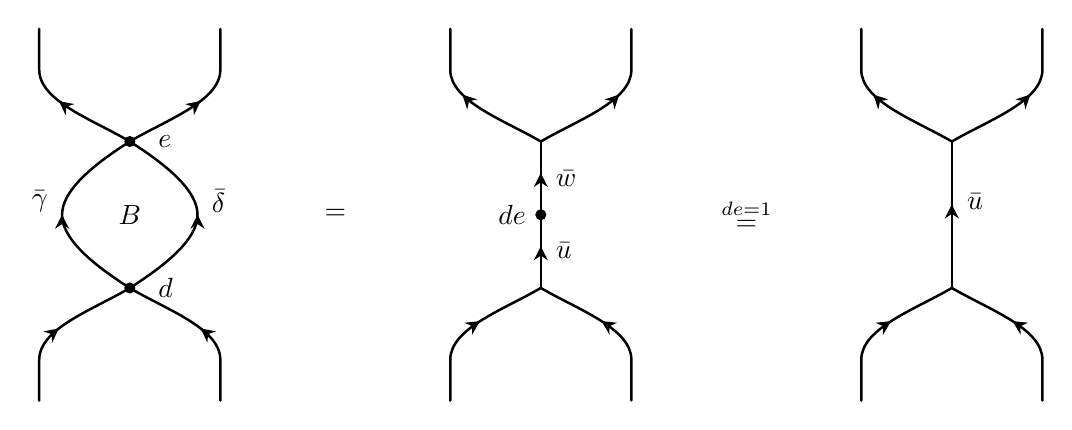
\begin{tikzpicture}[x=1cm,y=1cm,
 r2 two crossings up/.style={wire,decoration={markings,
   mark=at position .15 with {\arrow{Stealth[length=5pt,width=5pt]}},
   mark=at position .50 with {\arrow{Stealth[length=5pt,width=5pt]}},
   mark=at position .85 with {\arrow{Stealth[length=5pt,width=5pt]}}},
   postaction={decorate}}]
 \foreach \side in {-1,1} {
  \begin{scope}[xscale=\side]
   \draw[r2 two crossings up] (-1.15,-2.36) -- (-1.15,-1.84)
    .. controls (-1.15,-1.44) and (-.45,-1.20) .. (0,-.93)
    .. controls (.52,-.60) and (.86,-.29) .. (.86,0)
    .. controls (.86,.29) and (.52,.60) .. (0,.93)
    .. controls (-.45,1.20) and (-1.15,1.44) .. (-1.15,1.84)
    -- (-1.15,2.36);
  \end{scope}
 }
 \fill (0,-.93) circle (2pt);
 \fill (0,.93) circle (2pt);
 \node[strandlabel,anchor=west] at (.31,-.93) {$d$};
 \node[strandlabel,anchor=west] at (.31,.93) {$e$};
 \node[region] at (0,0) {$B$};
 \node[strandlabel,anchor=east] at (-.99,.17) {$\bar\gamma$};
 \node[strandlabel,anchor=west] at (.99,.17) {$\bar\delta$};
 \rTwoBoundary
 \node at (2.61,0) {$=$};
 \newcommand{\rTwoMergeSplit}[1]{%
  \draw[oriented] (-1.15,-2.36)--(-1.15,-1.84)
    .. controls (-1.15,-1.44) and (-.46,-1.20) .. (0,-.93);
  \draw[oriented] (1.15,-2.36)--(1.15,-1.84)
    .. controls (1.15,-1.44) and (.46,-1.20) .. (0,-.93);
  \ifnum#1=1
    \draw[oriented] (0,-.93)--(0,0);
    \draw[oriented] (0,0)--(0,.93);
    \fill (0,0) circle (2pt);
    \node[strandlabel,anchor=east] at (-.14,0) {$de$};
    \node[strandlabel,anchor=west] at (.14,-.46) {$\bar u$};
    \node[strandlabel,anchor=west] at (.14,.46) {$\bar w$};
  \else
    \draw[oriented] (0,-.93)--(0,.93);
    \node[strandlabel,anchor=west] at (.14,.17) {$\bar u$};
  \fi
  \draw[oriented] (0,.93)
    .. controls (-.46,1.20) and (-1.15,1.44) .. (-1.15,1.84)
    --(-1.15,2.36);
  \draw[oriented] (0,.93)
    .. controls (.46,1.20) and (1.15,1.44) .. (1.15,1.84)
    --(1.15,2.36);
  \rTwoBoundary
 }
 \begin{scope}[xshift=5.22cm]
   \rTwoMergeSplit{1}
 \end{scope}
 \node at (7.83,0) {$\overset{de=1}{=}$};
 \begin{scope}[xshift=10.44cm]
   \rTwoMergeSplit{0}
 \end{scope}
\end{tikzpicture}
\end{center}

\begin{theorem}[Parallel Reidemeister II]\label{thm:r2-parallel}
Two induction crossings labelled \(d,e\), read bottom to top, equal
a merge, a dot \(de\) from \(\bar u\) to \(\bar w\), and a split.
For \(de=1\) the merged labels agree and the dot disappears.
The remaining map is the identity if both boundary sequences agree.
Each group-element label \(d\) has an admissible return label \(d^{-1}\).
\end{theorem}

\begin{proof}
The three merges identify the tensor products with copies of
\(\C[G]\), with right actions through \(u_*,v_*,w_*\).
The split and merge on the middle product cancel, leaving
\(x\mapsto xd\mapsto xde\).
For group-element dots \(u^{-1}dv\) and \(v^{-1}ew\) centralize
\(K\), so their product \(u^{-1}de\,w\) does too. The same test
applies to each product of terms in linear labels.
If \(de=1\), then \(u^{-1}w\in C_U(K)\), so the merged strand
stays the same through the dot. If the boundaries agree, the
top split inverts the bottom merge.
Finally \(v^{-1}d^{-1}u=(u^{-1}dv)^{-1}\) proves admissibility
for the return dot. Both products of \(d,d^{-1}\) equal \(1\).
\end{proof}

For two restriction strands, the group-element labels act on the
left, giving \(x\mapsto d^{-1}x\mapsto e^{-1}d^{-1}x=(de)^{-1}x\).
The product label is again \(de\), including for linear labels by
expansion in group elements.

\Needspace{26\baselineskip}
\section{Reidemeister III move}\label{sec:reidemeister-three}

With the boundary fixed, we determine when one three-crossing shape
can replace the other. We treat three induction strands and the six
directions of replacement with one restriction strand, including
cases that require a sum or admit no replacement.

\subsection{Three induction strands}

For the standard inclusions \(S_n\subset S_{n+1}\), Khovanov obtains
the three-upward-strand braid relation from the relation for adjacent
transpositions \cite[Prop.~7]{khovanov}.

All strands point up. For adjacent groups \(X,Y\le U\),
\(\boxed{XY}\) represents the label \(\boxed{XY}C_U(Y)\).
Fix the six outer groups and the six boundary strand labels shown
below.

\begin{center}
\newcommand{\reidemeisterthreewires}{%
 \draw[arrowatend] (-1.70,-2.50)--(-1.70,-1.98)
   .. controls (-1.70,-1.60) and (0,-1.36) .. (0,-.98)
   --(0,-.50)
   .. controls (0,-.12) and (1.70,.12) .. (1.70,.50)
   --(1.70,2.50);
 \draw[arrowatend] (0,-2.50)--(0,-1.98)
   .. controls (0,-1.60) and (-1.70,-1.36) .. (-1.70,-.98)
   --(-1.70,.98)
   .. controls (-1.70,1.36) and (0,1.60) .. (0,1.98)
   --(0,2.50);
 \draw[arrowatend] (1.70,-2.50)--(1.70,-.50)
   .. controls (1.70,-.12) and (0,.12) .. (0,.50)
   --(0,.98)
   .. controls (0,1.36) and (-1.70,1.60) .. (-1.70,1.98)
   --(-1.70,2.50);
 \fill (-.85,-1.48) circle (2.1pt);
 \fill (.85,0) circle (2.1pt);
 \fill (-.85,1.48) circle (2.1pt);
}%
\newcommand{\reidemeisterthreeboundary}{%
 \node[region] at (-2.22,-.10) {$G$};
 \node[region] at (2.22,-.10) {$F$};
 \node[region] at (-.85,-2.26) {$A$};
 \node[region] at (.85,-2.26) {$D$};
 \node[region] at (-.85,2.26) {$C$};
 \node[region] at (.85,2.26) {$E$};
 \foreach \xpos/\bottomlabel/\toplabel in {
   -1.70/GA/GC,0/AD/CE,1.70/DF/EF} {
   \node[strandlabel,anchor=north] at (\xpos,-2.66)
     {$\co{\boxed{\bottomlabel}}$};
   \node[strandlabel,anchor=south] at (\xpos,2.66)
     {$\co{\boxed{\toplabel}}$};
 }
}%
\begin{tikzpicture}[x=1cm,y=1cm]
 \reidemeisterthreewires
 \reidemeisterthreeboundary
 \node[region] at (-.82,0) {$B$};
 \node[strandlabel,anchor=east] at (-1.88,.69) {$\co{\boxed{GB}}$};
 \node[strandlabel,anchor=east] at (-.14,-.74) {$\co{\boxed{BD}}$};
 \node[strandlabel,anchor=east] at (-.14,.74) {$\co{\boxed{BE}}$};
 \node[strandlabel,anchor=east] at (-1.20,-1.48) {$x_1$};
 \node[strandlabel,anchor=west] at (1.20,0) {$x_2$};
 \node[strandlabel,anchor=east] at (-1.20,1.48) {$x_3$};
 \node at (3.65,0) {$\longleftrightarrow$};
 \begin{scope}[xshift=7.30cm]
   \begin{scope}[xscale=-1]
     \reidemeisterthreewires
   \end{scope}
   \reidemeisterthreeboundary
   \node[region] at (.82,0) {$B'$};
   \node[strandlabel,anchor=west] at (1.88,.69) {$\co{\boxed{B'F}}$};
   \node[strandlabel,anchor=west] at (.14,-.74) {$\co{\boxed{AB'}}$};
   \node[strandlabel,anchor=west] at (.14,.74) {$\co{\boxed{CB'}}$};
   \node[strandlabel,anchor=west] at (1.20,-1.48) {$y_1$};
   \node[strandlabel,anchor=east] at (-1.20,0) {$y_2$};
   \node[strandlabel,anchor=west] at (1.20,1.48) {$y_3$};
 \end{scope}
\end{tikzpicture}
\end{center}

\paragraph{Diagrams and their classes.}
Let \(\mathcal L,\mathcal R\) be the admissible labellings of the left
and right shapes at this boundary. A labelling specifies the middle
group, the three interior strand cosets, and the three crossing
dots. Each crossing merges, applies its dot, and splits. A dot
can be a finite \(\C\)-linear combination of the group elements
allowed between the two merged strand labels.

Write \(\operatorname{ev}(\mathsf D)\) for the resulting map from the
bottom tensor product to the top one. Within each shape let
\(\mathsf D\sim\mathsf E\) mean
\(\operatorname{ev}(\mathsf D)=\operatorname{ev}(\mathsf E)\), and write
\([\mathsf D]\) for the equivalence class of \(\mathsf D\).

\paragraph{Multipliers.}
Choose boundary representatives and put
\[
 u=\boxed{GA}\boxed{AD}\boxed{DF},\qquad
 v=\boxed{GC}\boxed{CE}\boxed{EF}.
\]
Merging the bottom and top products gives \(\C[G]\) with right
\(\C[F]\)-actions through \(u_*,v_*\). Every left \(\C[G]\)-linear map
is right multiplication by its value at \(1\), denoted \(m(\mathsf D)\).
At the fixed boundary, equality of these values is equality of maps.

\begin{lemma}[Multipliers under relabelling]\label{lem:reidemeister-three}
At the fixed boundary there are constructions \(\phi:\mathcal L\to\mathcal R\)
and \(\psi:\mathcal R\to\mathcal L\) preserving the multiplier of every
input diagram. Their two round trips satisfy
\[
 m(\psi(\phi(\mathsf D)))=m(\mathsf D)\quad(\mathsf D\in\mathcal L),
 \qquad
 m(\phi(\psi(\mathsf D)))=m(\mathsf D)\quad(\mathsf D\in\mathcal R).
\]
\end{lemma}

\begin{proof}
For a single
\(p\in G\), the right \(\C[F]\)-linearity condition is
\[
 u f u^{-1}p=p v f v^{-1}\quad(f\in F)
 \quad\Longleftrightarrow\quad u^{-1}pv\in C_U(F).
\]
At a crossing of the left pair, let \(\lambda_*,\mu_*\) be the
incoming and outgoing merged embeddings into \(G\), and let \(d\)
be the dot. Merging with the third strand after applying the dot
gives \(zd\mu_*(w)=z\lambda_*(w)d\), so the multiplier is \(d\).
At a crossing of the right pair, the left embedding \(\gamma_*\)
sends the dot to \(\gamma_*(d)\) because
\(z\gamma_*(wd)=z\gamma_*(w)\gamma_*(d)\). Hence the multipliers are
\[
 \begin{aligned}
 \text{left}\quad &x_1(\boxed{GB})_*(x_2)x_3,\\
 \text{right}\quad &(\boxed{GA})_*(y_1)y_2(\boxed{GC})_*(y_3).
 \end{aligned}
\]
Expand the three labels into group elements. Each triple gives a
bimodule map whose multiplier is a single group element \(p\).
Thus \(u^{-1}pv\in C_U(F)\) for every \(p\) in the support of \(m\),
the group elements with nonzero coefficient.

\Needspace{14\baselineskip}
\paragraph{Construction of \(\phi\).}
Given a left-hand diagram with multiplier \(m\), choose the right-hand
internal group \(B'=F\) and take
\[
 \boxed{B'F}=1,\qquad
 \boxed{AB'}=\boxed{AD}\boxed{DF},\qquad
 \boxed{CB'}=\boxed{CE}\boxed{EF}.
\]
The outer vertices compare equal embeddings into \(A\) and \(C\),
so take \(y_1=y_3=1\). At the middle vertex, \(pv\) represents
\(\bar u\) for every \(p\) in the support of \(m\), since \(u^{-1}pv\in C_U(F)\).
Using \(v\) for the outgoing label gives the dot
\((pv)v^{-1}=p\). Thus \(y_2=m\) is allowed and gives multiplier \(m\).

\paragraph{Construction of \(\psi\).}
Given a right-hand diagram with multiplier \(m\), choose the left-hand
internal group \(B=G\) and take
\[
 \boxed{GB}=1,\qquad
 \boxed{BD}=\boxed{GA}\boxed{AD},\qquad
 \boxed{BE}=\boxed{GC}\boxed{CE}.
\]
The outer vertices compare equal embeddings of \(D\) and \(E\)
into \(G\), so take \(x_1=x_3=1\). The middle vertex compares
\(u_*,v_*\) into \(B=G\). The same representatives \(pv,v\)
allow \(x_2=m\). The left strand is the inclusion \(G\to G\),
so the multiplier is \(m\).

\paragraph{Round-trip calculations.}
After the first step the multiplier is still \(m(\mathsf D)\).
Returning to the left gives \(B=G\) and dots
\((1,m(\mathsf D),1)\). Returning to the right gives \(B'=F\)
and the same dot triple. Substitution gives
\begin{equation*}
\begin{aligned}
 m(\psi(\phi(\mathsf D)))&=1\cdot m(\mathsf D)\cdot1
    =m(\mathsf D) &&(\mathsf D\in\mathcal L),\\
 m(\phi(\psi(\mathsf D)))&=(\boxed{GA})_*(1)\,m(\mathsf D)\,(\boxed{GC})_*(1)
    =m(\mathsf D) &&(\mathsf D\in\mathcal R).
\end{aligned}
\qedhere
\end{equation*}
\end{proof}

\Needspace{7\baselineskip}
\begin{theorem}[Reidemeister III]\label{thm:reidemeister-three}
At the fixed boundary, the constructions of Lemma~\ref{lem:reidemeister-three}
induce mutually inverse bijections
\[
 \mathcal L/{\sim}\longrightarrow\mathcal R/{\sim},
 \quad [\mathsf D]\longmapsto[\phi(\mathsf D)],
 \qquad
 \mathcal R/{\sim}\longrightarrow\mathcal L/{\sim},
 \quad [\mathsf D]\longmapsto[\psi(\mathsf D)].
\]
The induced maps are independent of the internal labellings chosen
in any construction preserving the boundary and evaluated map.
\end{theorem}

\begin{proof}
If \(\mathsf D\sim\mathsf E\) on the left, the lemma gives
\(m(\phi(\mathsf D))=m(\mathsf D)=m(\mathsf E)=m(\phi(\mathsf E))\),
so the outputs are equivalent. The same argument applies to
\(\psi\). Any other output with the same shape, boundary, and
multiplier gives the same class. The two round-trip equalities
in the lemma therefore give the identity on each set of classes.
\end{proof}


\begin{example}[A round trip with different labels]\label{ex:induction-round-trip}
Take every group to be \(C_2=\{1,g\}\) and every strand to carry the
identity embedding. The left diagram \(\mathsf D\) with dots \((g,1,g)\)
has multiplier \(g^2=1\). Its round trip \(\mathsf D'=\psi(\phi(\mathsf D))\)
has dots \((1,1,1)\). Both diagrams give the identity bimodule map.
Since \(\phi\) uses only the multiplier at this boundary,
\(\phi(\mathsf D)=\phi(\mathsf D')\). One return rule cannot recover
both inputs. Starting on the right gives the same obstruction for \(\psi\).
\end{example}

\Needspace{17\baselineskip}
\paragraph{Other choices of internal group.}
For \(\psi\) one may use any \(B\le G\) containing
\(\cg{\boxed{GA}}{A}\), \(\cg{\boxed{GC}}{C}\), and all group elements
with nonzero coefficient in \(m\). The outer embeddings still agree
and the inclusion sends \(m\in \C[B]\) to the same multiplier.

For \(\phi\) with group-element labels, choose representatives at
each crossing. A representative \(\alpha\beta c\) of a composite
coset factors as \(\alpha(\beta c)\), so the choices can be made on
the strands themselves. This gives
\begin{align*}
 x_1&=\boxed{GA}\boxed{AD}\boxed{BD}^{-1}\boxed{GB}^{-1},\\
 x_2&=\boxed{BD}'\boxed{DF}\boxed{EF}^{-1}\boxed{BE}^{-1},\\
 x_3&=\boxed{GB}'\boxed{BE}'\boxed{CE}^{-1}\boxed{GC}^{-1}.
\end{align*}
Primes denote other representatives of the same internal labels.
Each boundary strand meets one vertex, so use its chosen
representative in \(u,v\). Both \(\boxed{GB}\) and \(\boxed{GB}'\)
act the same way on \(B\). For
\(p=x_1\boxed{GB}x_2\boxed{GB}^{-1}x_3\), cancellation gives
\[
 \begin{aligned}
 u^{-1}pv={}&
 \bigl(\boxed{DF}^{-1}\boxed{BD}^{-1}\boxed{BD}'\boxed{DF}\bigr)\\
 &{}\cdot
 \bigl(\boxed{EF}^{-1}\boxed{BE}^{-1}\boxed{GB}^{-1}
       \boxed{GB}'\boxed{BE}'\boxed{EF}\bigr).
 \end{aligned}
\]
The first factor centralizes \(\cg{\boxed{DF}^{-1}}{D}\).
In the second, \(\boxed{GB}^{-1}\boxed{GB}'\) centralizes
\(B\), which contains \(\cg{\boxed{BE}}{E}\), and
\(\boxed{BE}^{-1}\boxed{BE}'\) centralizes \(E\). Thus the
second factor centralizes \(\cg{\boxed{EF}^{-1}}{E}\).
Both factors centralize
\[
 B''=\cg{\boxed{DF}^{-1}}{D}\cap\cg{\boxed{EF}^{-1}}{E}.
\]
It contains \(F\). Take \(B'=\cg{\tau}{B''}\) for any \(\tau\in U\)
and use
\[
 \boxed{B'F}=\tau,\qquad
 \boxed{AB'}=\boxed{AD}\boxed{DF}\tau^{-1},\qquad
 \boxed{CB'}=\boxed{CE}\boxed{EF}\tau^{-1}.
\]
The inclusions in the definition of \(B''\) and \(F\le B''\)
give these three embeddings. The outer composites agree, so
\(y_1=y_3=1\). At the middle vertex
\((u\tau^{-1})^{-1}p(v\tau^{-1})=\tau(u^{-1}pv)\tau^{-1}\)
centralizes \(B'\), so \(y_2=p\) gives the original multiplier.


\Needspace{9\baselineskip}
\subsection{One restriction strand on the outside}\label{sec:outside-restriction}

Number the three positions from left to right at the bottom.
Read the diagrams from bottom to top. The crossing \(s_1\) exchanges
positions \(1\) and \(2\), and \(s_2\) exchanges positions \(2\) and \(3\).

\begin{center}
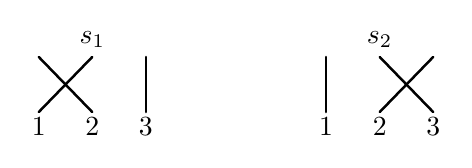
\begin{tikzpicture}[x=.68cm,y=.70cm]
  \draw[wire] (0,0)--(1,1);
  \draw[wire] (1,0)--(0,1);
  \draw[wire] (2,0)--(2,1);
  \node[strandlabel] at (1,1.31) {$s_1$};
  \begin{scope}[xshift=3.65cm]
    \draw[wire] (0,0)--(0,1);
    \draw[wire] (1,0)--(2,1);
    \draw[wire] (2,0)--(1,1);
    \node[strandlabel] at (1,1.31) {$s_2$};
  \end{scope}
  \foreach \position in {0,1,2} {
    \pgfmathtruncatemacro{\numberlabel}{\position+1}
    \node[strandlabel] at (\position,-.26) {$\numberlabel$};
    \node[strandlabel,xshift=3.65cm] at (\position,-.26) {$\numberlabel$};
  }
\end{tikzpicture}
\end{center}

In each pair below, the left shape is \(s_1s_2s_1\) and the right shape is
\(s_2s_1s_2\). The numbers identify the direction of replacement.
Fix the boundary groups and the boundary strand cosets in each pair.
Letters such as \(a\) denote conjugation embeddings, and \(\bar a\) is
the coset of a representative of \(a\). Write \(ad=a\circ d\).
Write \(\operatorname{Ad}_p\) for conjugation by \(p\).

A label \(s\) on a mixed crossing denotes the parameter in
\(q_s([k,h])=\alpha(k)s\beta(h)\). The multiplication crossing is
\(q_s\). The projection uses the trace dot \(s^{-1}\) and sends
\[
 z\longmapsto q_s^!(z)=\sum_{q_s([k,h])=z}[k,h].
\]
By Proposition~\ref{prop:r2-mixed-composition}, this formula applies
when the fibers of \(q_s\) are finite, even if the cup by itself
would have infinite index. In a composite with linear labels,
each projection must have finite fibers for every term used.

\Needspace{19\baselineskip}
\subsubsection{Cases 1 and 2. Both mixed crossings are projections}

\begin{center}
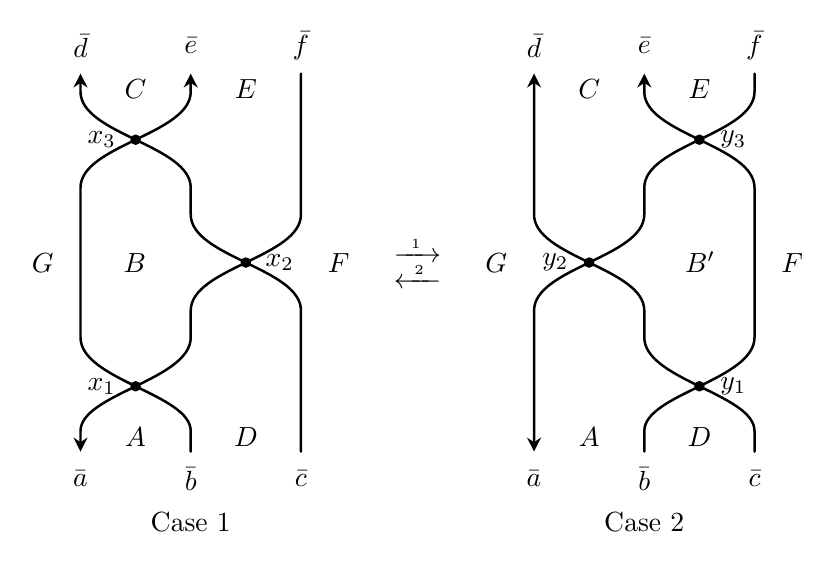
\begin{tikzpicture}
  \mixedThreeWires{arrowatstart}{arrowatend}{arrowatend}
  \mixedThreeLeft
  \mixedThreeBoundary{A}{D}{C}{E}{0/a,1.4/b,2.8/c}{0/d,1.4/e,2.8/f}{1}
  \node at (4.28,2.4) {$\substack{\xrightarrow{\ 1\ }\\[-.2ex]\xleftarrow{\ 2\ }}$};
  \begin{scope}[xshift=5.76cm]
    \begin{scope}[shift={(2.8,0)},xscale=-1]
      \mixedThreeWires{arrowatend}{arrowatend}{arrowatstart}
    \end{scope}
    \mixedThreeRight
    \mixedThreeBoundary{A}{D}{C}{E}{0/a,1.4/b,2.8/c}{0/d,1.4/e,2.8/f}{2}
  \end{scope}
\end{tikzpicture}
\end{center}

The lower embeddings are \(a:G\to A\), \(b:D\to A\), and \(c:F\to D\).
The upper ones are \(d:C\to G\), \(e:E\to C\), and \(f:E\to F\).
After merging parallel strands, the bottom basis is \(A\), with actions
through \(a,bc\). The top basis is \(G\times_E F\), balanced using \(de,f\).

\begin{lemma}[Evaluation for two projections]\label{lem:three-projections}
With a group element at each vertex, either shape evaluates to
\(Q_p^!\), the sum over the fibers of
\[
 Q_p([g,h])=a(g)p(bc)(h),\qquad [g,h]\in G\times_E F,
\]
for a unique \(p\in A\). Its admissibility condition and fiber size over its image are
\begin{equation}\label{eq:three-projection-index}
 \begin{gathered}
 (ade)(v)p=p(bcf)(v)\qquad(v\in E),\\
 n_p=[a(G)\cap p(bc)(F)p^{-1}:(ade)(E)]<\infty .
 \end{gathered}
\end{equation}
A diagram with linear labels evaluates to a finite linear combination
of these \(Q_p^!\). Its coefficients are determined by the evaluated map.
\end{lemma}

\begin{proof}
On the left, write \(r:B\to G\), \(s:B\to D\), and \(t:E\to B\).
Use \(x,y\) for the first two mixed crossing elements and \(z\) for the upper
induction dot. Following the underlying set maps backwards gives
\[
 \begin{aligned}
 {[g,h]}&\longmapsto[gz^{-1},h]\longmapsto[gz^{-1},y c(h)]\\
      &\longmapsto a(gz^{-1})x\,b(yc(h)).
 \end{aligned}
\]
Thus \(p=a(z^{-1})x b(y)\). On the right use
\(u:B'\to A\), \(v:C\to B'\), and \(w:F\to B'\), with induction dot \(\ell\)
and mixed crossing elements \(m,n\). The set maps give
\[
 \begin{aligned}
 {[g,h]}&\longmapsto[g,nw(h)]\longmapsto a(g)m\,u(nw(h))\\
      &\longmapsto a(g)m\,u(nw(h))\ell^{-1}.
 \end{aligned}
\]
Thus \(p=m u(n)\ell^{-1}\). Taking inverse images twice gives the fiber of the composite.
These fibers are finite because each projection has finite fibers. Balancing gives the first condition in
\eqref{eq:three-projection-index}. The stabilizer index calculation in
Proposition~\ref{prop:r2-mixed-composition} gives \(n_p\).
Expanding the three labels proves the linear formula. The coefficient
of \([1,1]\) in \(Q_p^!(z)\) is \(1\) for \(z=p\) and \(0\) otherwise,
so the coefficient of each \(Q_p^!\) can be recovered.
\end{proof}

\begin{theorem}[Replacement for two projections]\label{thm:three-projections}
For \(p\) satisfying \eqref{eq:three-projection-index}, put
\(P_p=\langle (ad)(C),p(bc)(F)p^{-1}\rangle\le A\).
\begin{enumerate}
\item In Case~1, a finite sum of right diagrams gives the same map as
the left diagram exactly when each \(p\) with nonzero coefficient satisfies
\begin{equation}\label{eq:three-middle-index}
 [a(G)\cap P_p:(ad)(C)]<\infty.
\end{equation}
Each such \(Q_p^!\) has a single right diagram.
If \([G:d(C)]<\infty\), one right diagram suffices for the whole sum.
\item In Case~2, every right diagram has a replacement by a finite sum
of left diagrams. If \([G:(de)(E)]<\infty\), one left diagram suffices.
\end{enumerate}
Under \([G:(de)(E)]<\infty\), in particular for finite groups, the
single-diagram replacements induce inverse bijections on the two
sets of classes modulo equality of evaluated maps.
\end{theorem}

\begin{proof}
For Case~1, the three vertex conditions on the right are
\[
 \begin{gathered}
 bc=\operatorname{Ad}_{\ell}\circ uw,\qquad
 ad=\operatorname{Ad}_{m}\circ uv,\\
 ve=\operatorname{Ad}_{n}\circ wf .
 \end{gathered}
\]
By \(p=m u(n)\ell^{-1}\), the group \(m u(B')m^{-1}\)
contains \(P_p\). Its intersection with \(a(G)\) has finite index
over \((ad)(C)\), since that index is the middle fiber size.
This proves necessity for each term. The coefficient test in
Lemma~\ref{lem:three-projections} gives necessity for finite sums.

For sufficiency take \(B'=P_p\), \(u\) the inclusion, \(v=ad\),
\(w=\operatorname{Ad}_p\circ bc\), and \((\ell,m,n)=(p^{-1},1,1)\).
The first vertex satisfies \(bc=\operatorname{Ad}_{p^{-1}}\circ uw\).
The middle fiber is finite by \eqref{eq:three-middle-index}.
The upper vertex uses \(ve=wf\), and its index is at most \(n_p\)
because \((ad)(C)\le a(G)\). If \([G:d(C)]\) is finite, take a
common \(B'=A,\ u=\id,\ v=ad,\ w=bc\). Put the linear combination
of crossing elements on the upper mixed crossing and use \(1\) at the first two.
The middle fiber then has size \([G:d(C)]\), and the upper fiber
of each crossing element has size at most \(n_p\).

For Case~2 use the full intersection at the first crossing.
\[
 \begin{gathered}
 B=a^{-1}\bigl(a(G)\cap p b(D)p^{-1}\bigr),\qquad r=\mathrm{incl},\\
 s=b^{-1}\circ\operatorname{Ad}_{p^{-1}}\circ a\bigm|_B,\qquad t=de.
 \end{gathered}
\]
Use \((x,y,z)=(p,1,1)\). Equation~\eqref{eq:three-projection-index}
gives \(st=cf\). The first fiber has size \(1\) on its image.
Transporting the second intersection by \(\operatorname{Ad}_p\circ b\)
gives the index \(n_p\). This produces one left diagram per crossing element.
If \([G:(de)(E)]<\infty\), take a common \(B=E,\ r=de,\ s=cf,\ t=\id\)
and put the linear combination of crossing elements on the lower mixed crossing.
For each crossing element the first fiber size is bounded by \([G:(de)(E)]\),
and the second has size \(1\).

In the two-way case both constructions preserve evaluation.
Equivalent inputs therefore give equivalent outputs, and each
round trip returns to the original shape with the original map.
This proves the asserted inverses on classes.
\end{proof}


\begin{example}[A Case 1 diagram with no finite right replacement]\label{ex:case-one-no-finite-replacement}
Take \(U=A=\mathbb Z^2\rtimes C_2\), where \(C_2\) swaps the two
coordinate lines. Set \(G=\mathbb Z^2\), \(C=\mathbb Z\times\{0\}\),
\(D=F=C_2\), and \(B=E=1\). Use inclusions and unit labels on the left. Both
reverse cups have index \(2\), and \(Q_1^!(gh)=[g,h]\) for \(g\in G,\ h\in F\).
However \(P_1=\langle C,F\rangle=A\) because the swap conjugates \(C\) to the
other coordinate line. The index in \eqref{eq:three-middle-index} is
\([G:C]=\infty\).
\end{example}


\begin{example}[A Case 2 diagram requiring a sum]\label{ex:case-two-needs-a-sum}
In the same semidirect product write \(\tau\) for the swap.
Set \(G=D=\mathbb Z\times\{0\}\) and \(C=E=F=B'=1\). Use inclusions on
the right, with dots \((1,1+\tau,1)\). Both right-hand reverse cups
have index \(1\). The resulting map \(Q_1^!+Q_\tau^!\) is nonzero on
both \(1\) and \(\tau\). A left replacement must use parameters at the
first crossing in both \(G\) and \(G\tau G\), since \(p=a(z^{-1})x b(y)\) is
in the same double coset as that crossing's crossing element \(x\). The
corresponding intersections are \(G\) and \(1\). The crossing element in
\(G\tau G\) forces \(B=1\), giving the crossing element in \(G\) infinite fibers.
\end{example}

\Needspace{19\baselineskip}
\subsubsection{Cases 3 and 4. Both mixed crossings are multiplications}

\begin{center}
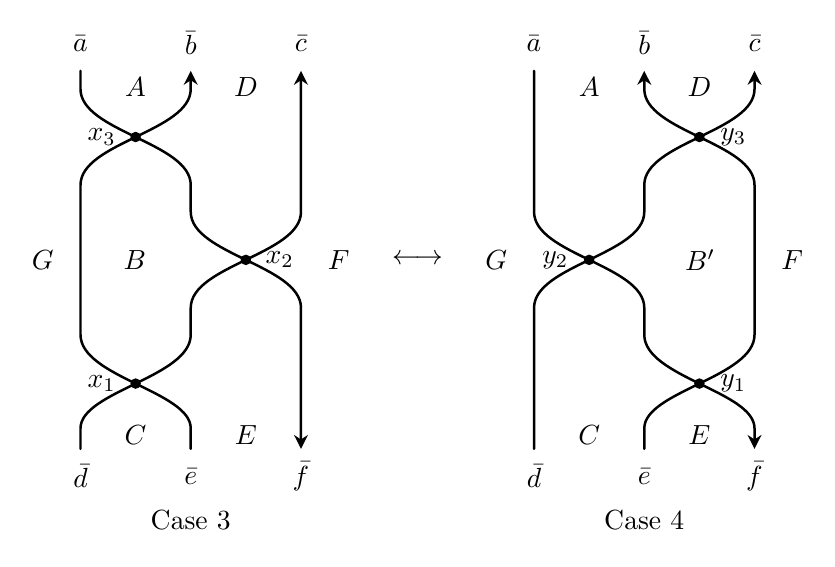
\begin{tikzpicture}
  \mixedThreeWires{arrowatend}{arrowatend}{arrowatstart}
  \mixedThreeLeft
  \mixedThreeBoundary{C}{E}{A}{D}{0/d,1.4/e,2.8/f}{0/a,1.4/b,2.8/c}{3}
  \node at (4.28,2.4) {$\longleftrightarrow$};
  \begin{scope}[xshift=5.76cm]
    \begin{scope}[shift={(2.8,0)},xscale=-1]
      \mixedThreeWires{arrowatstart}{arrowatend}{arrowatend}
    \end{scope}
    \mixedThreeRight
    \mixedThreeBoundary{C}{E}{A}{D}{0/d,1.4/e,2.8/f}{0/a,1.4/b,2.8/c}{4}
  \end{scope}
\end{tikzpicture}
\end{center}

The boundary embeddings from Cases~1 and~2 exchange top and bottom.
The source basis is \(G\times_E F\) and the target basis is \(A\).

\begin{theorem}[Replacement for two multiplications]\label{thm:three-multiplications}
At arbitrary index, either shape evaluates to
\[
 [g,h]\longmapsto a(g)M(bc)(h),
\]
where \(M\in\C[A]\) is a finite complex linear combination of group elements \(p\) satisfying
\((ade)(v)p=p(bcf)(v)\) for \(v\in E\).
Every such \(M\) is realized by a single diagram of either shape.
The two replacements induce inverse bijections on classes modulo
equality of evaluated maps.
\end{theorem}

\begin{proof}
The two backward calculations in Lemma~\ref{lem:three-projections}
now run from bottom to top. Each mixed crossing applies its map
\(q_s\), and the parallel-strand crossing acts by the corresponding
merge, dot and split. Each group-element triple gives \(Q_p\).
Expansion gives the formula with \(M\), which is the value at \([1,1]\).

In Case~3 take \(B'=A,\ u=\id,\ v=ad,\ w=bc\). Put the label \(M\)
at the bottom mixed crossing and \(1\) at the other two. For each term
\(p\) of \(M\) the first multiplication gives \([g,p(bc)(h)]\).
The next multiplication and the last merge and split give
\(a(g)p(bc)(h)\). In Case~4 take \(B=E,\ r=de,\ s=cf,\ t=\id\).
Put \(M\) at the top mixed crossing and \(1\) at the other two.
The first merge and split and the next multiplication give \([g,c(h)]\).
The last multiplication gives \(a(g)p b(c(h))\) for each term \(p\).
In both constructions the condition on \(p\) is exactly the condition
at its vertex. All mixed crossings are multiplication maps, so no
index condition enters.

Equality of \(M\) is equality of evaluated maps. The constructions
preserve \(M\), so they are well defined on classes and each round
trip is the identity on its set of classes.
\end{proof}


\begin{example}[A round trip for two mixed multiplications]\label{ex:multiplication-round-trip}
The round trip may change the labels. With every group \(C_2=\{1,g\}\)
and every embedding the identity, the left diagram with labels
\((g,1,g)\) has \(M=1\). Its round trip has labels \((1,1,1)\)
and the same map.
\end{example}

\Needspace{19\baselineskip}
\subsection{One restriction strand in the middle}

\begin{center}
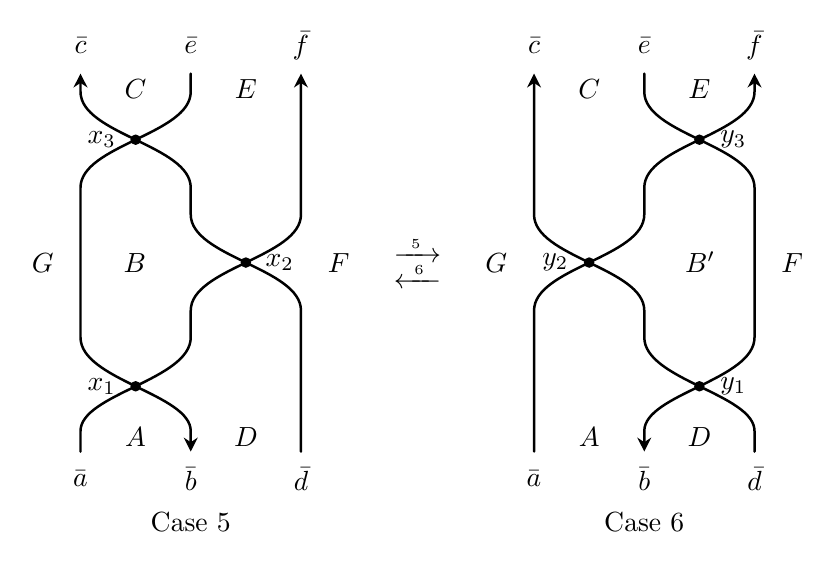
\begin{tikzpicture}
  \mixedThreeWires{arrowatend}{arrowatstart}{arrowatend}
  \mixedThreeLeft
  \mixedThreeBoundary{A}{D}{C}{E}{0/a,1.4/b,2.8/d}{0/c,1.4/e,2.8/f}{5}
  \node at (4.28,2.4) {$\substack{\xrightarrow{\ 5\ }\\[-.2ex]\xleftarrow{\ 6\ }}$};
  \begin{scope}[xshift=5.76cm]
    \begin{scope}[shift={(2.8,0)},xscale=-1]
      \mixedThreeWires{arrowatend}{arrowatstart}{arrowatend}
    \end{scope}
    \mixedThreeRight
    \mixedThreeBoundary{A}{D}{C}{E}{0/a,1.4/b,2.8/d}{0/c,1.4/e,2.8/f}{6}
  \end{scope}
\end{tikzpicture}
\end{center}

Write \(a:A\to G\), \(b:A\to D\), and \(d:F\to D\) for the lower
embeddings and \(c:C\to G\), \(e:C\to E\), and \(f:F\to E\) for the upper ones.
The source basis is \(G\times_A D\) and the target basis is \(G\times_C E\).

\begin{lemma}[Evaluation with one projection]\label{lem:three-middle-restriction}
On the left use \(u:G\to B\), \(v:D\to B\), and \(w:E\to B\),
and labels \(r,t,s\) from bottom to top, with \(r,s\) the mixed crossing elements.
The map is
\begin{equation}\label{eq:three-left-middle-restriction}
 [g,x]_A\longmapsto
 \sum_{\substack{[h,y]_C\\u(h)s w(y)=u(g)r v(x)t}}[h,y]_C .
\end{equation}
On the right use \(i:B'\to A\), \(j:B'\to F\), and \(k:B'\to C\),
and write the labels in the same order as \(r,t,s\). The map is
\begin{equation}\label{eq:three-right-middle-restriction}
 [g,x]_A\longmapsto
 \sum_{\substack{[\alpha,h]\in A\times_{B'}F\\ b(\alpha)r d(h)=x}}
       [ga(\alpha)t,\ s f(h)]_C .
\end{equation}
For linear labels, sum the formulas over the group-element triples.
\end{lemma}

\begin{proof}
On the left the vertex conditions are
\[
 \begin{gathered}
 ua=\operatorname{Ad}_r\circ vb,\qquad
 vd=\operatorname{Ad}_t\circ wf,\qquad
 uc=\operatorname{Ad}_s\circ we .
 \end{gathered}
\]
The lower multiplication gives \(u(g)r v(x)\), the induction dot
right-multiplies by \(t\), and the upper projection takes the displayed
fiber. On the right the conditions are
\[
 \begin{gathered}
 bi=\operatorname{Ad}_r\circ dj,\qquad
 ai=\operatorname{Ad}_t\circ ck,\qquad
 ek=\operatorname{Ad}_s\circ fj .
 \end{gathered}
\]
The lower projection sums factorizations of \(x\) as \(b(\alpha)r d(h)\).
The induction dot sends the first coordinate of the surviving pair
to \(ga(\alpha)t\), and the upper multiplication sends the second
to \(s f(h)\).
\end{proof}

\subsubsection{Case 5. Replacement by sums of right diagrams}

\begin{theorem}[Expansion into right diagrams]\label{thm:three-orbits}
With this boundary, every bimodule map is a sum of right diagrams
under the finite-fiber convention, with only finitely many nonzero
terms on each input. A finite sum suffices exactly when only
finitely many \(G\times F\)-orbits of input--output basis pairs
have nonzero matrix coefficient. The group acts simultaneously
on the input and output.
\end{theorem}

\begin{proof}
Let \(G\times F\) act on each basis by left multiplication by \(G\)
and right multiplication by the inverse of \(F\), using the boundary
embeddings. The action on input--output pairs acts on both coordinates.
A bimodule map has constant matrix coefficient on each orbit.

Choose a representative \(([1,r]_A,[t,s]_C)\) of an orbit.
Let \(P\le F\) be the image of its stabilizer in \(F\).
In detail, \(h\in P\) exactly when there exist \(i(h)\in A,\ k(h)\in C\)
satisfying
\[
 \begin{gathered}
 r d(h)r^{-1}=b(i(h)),\qquad
 s f(h)s^{-1}=e(k(h)),\\
 a(i(h))=t c(k(h))t^{-1}.
 \end{gathered}
\]
These equations describe the stabilizer as the graph
\(\{(a(i(h)),h):h\in P\}\). They also make \(i,k\) conjugation
embeddings. Take \(B'=P,\ j\) the inclusion, and labels \((r,t,s)\).
The displayed equations are the three vertex conditions.

The pairs in the orbit have the form
\[
 \bigl([g',r d(h)]_A,\ [g't,s f(h)]_C\bigr)
 \qquad(g'\in G,\ h\in F).
\]
The source in this pair equals \([g,x]_A\) exactly when
\(g'=ga(\alpha)\) and \(x=b(\alpha)r d(h)\) for some \(\alpha\in A\).
Two such choices give the same pair exactly when they are equivalent
in \(A\times_P F\), by the full stabilizer description.
Thus \eqref{eq:three-right-middle-restriction} sums each output in
the orbit once. If this orbit has nonzero coefficient in a bimodule
map, it has finitely many outputs over each input, so the lower
projection is defined.

Conversely, \eqref{eq:three-right-middle-restriction} shows that a
group-element triple contributes to at most one orbit, irrespective
of the chosen internal group. Finite sums and finite linear labels
therefore involve finitely many orbits. The construction gives one
diagram for each orbit of nonzero coefficient. At each input only
finitely many of these diagrams contribute, because an element of
the target has finite support. This gives the asserted expansion.
\end{proof}

In the diagram, \(\mathcal S\) is the set of supported orbits,
\(P_{\mathcal O}\) is the projected pair stabilizer, and
\(c_{\mathcal O}\) is the matrix coefficient on the orbit.

\begin{center}
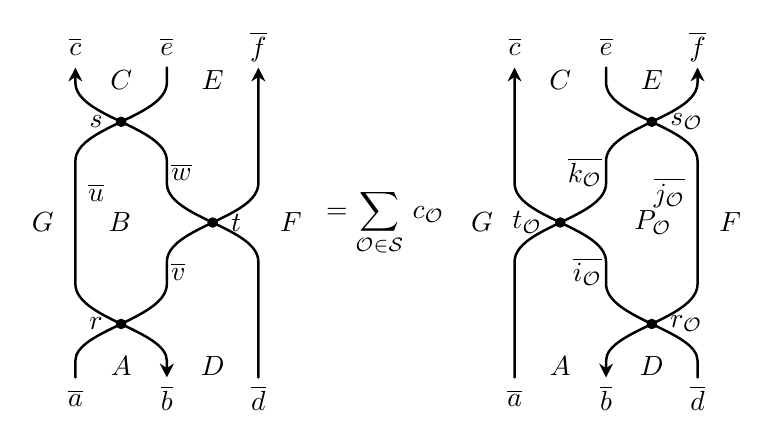
\begin{tikzpicture}[x=.83cm,y=.82cm]
\mixedThreeWires{arrowatend}{arrowatstart}{arrowatend}
\node[region] at (-0.5,2.4) {$G$};
\node[region] at (0.7,0.18) {$A$};
\node[region] at (2.1,0.18) {$D$};
\node[region] at (0.7,4.6) {$C$};
\node[region] at (2.1,4.6) {$E$};
\node[region] at (3.3,2.4) {$F$};
\node[strandlabel] at (0,-0.32) {$\overline{a}$};
\node[strandlabel] at (1.4,-0.32) {$\overline{b}$};
\node[strandlabel] at (2.8,-0.32) {$\overline{d}$};
\node[strandlabel] at (0,5.12) {$\overline{c}$};
\node[strandlabel] at (1.4,5.12) {$\overline{e}$};
\node[strandlabel] at (2.8,5.12) {$\overline{f}$};
\node[region] at (0.68,2.4) {$B$};
\fill (0.7,0.82875) circle (1.9pt);
\node[strandlabel,anchor=east] at (0.48,0.82875) {$r$};
\fill (2.1,2.4) circle (1.9pt);
\node[strandlabel,anchor=west] at (2.32,2.4) {$t$};
\fill (0.7,3.96) circle (1.9pt);
\node[strandlabel,anchor=east] at (0.48,3.96) {$s$};
\node[strandlabel,anchor=west] at (0.13,2.86) {$\overline{u}$};
\node[strandlabel,anchor=west] at (1.4,1.64) {$\overline{v}$};
\node[strandlabel,anchor=west] at (1.4,3.18) {$\overline{w}$};
\node at (4.74,2.4) {$=\displaystyle\sum_{\mathcal O\in\mathcal S}\,c_{\mathcal O}$};
\begin{scope}[shift={(6.72,0)}]
\begin{scope}[shift={(2.8,0)},xscale=-1]
\mixedThreeWires{arrowatend}{arrowatstart}{arrowatend}
\end{scope}
\node[region] at (-0.5,2.4) {$G$};
\node[region] at (0.7,0.18) {$A$};
\node[region] at (2.1,0.18) {$D$};
\node[region] at (0.7,4.6) {$C$};
\node[region] at (2.1,4.6) {$E$};
\node[region] at (3.3,2.4) {$F$};
\node[strandlabel] at (0,-0.32) {$\overline{a}$};
\node[strandlabel] at (1.4,-0.32) {$\overline{b}$};
\node[strandlabel] at (2.8,-0.32) {$\overline{d}$};
\node[strandlabel] at (0,5.12) {$\overline{c}$};
\node[strandlabel] at (1.4,5.12) {$\overline{e}$};
\node[strandlabel] at (2.8,5.12) {$\overline{f}$};
\node[region] at (2.12,2.4) {$P_{\mathcal O}$};
\fill (2.1,0.82875) circle (1.9pt);
\node[strandlabel,anchor=west] at (2.32,0.82875) {$r_{\mathcal O}$};
\fill (0.7,2.4) circle (1.9pt);
\node[strandlabel,anchor=east] at (0.48,2.4) {$t_{\mathcal O}$};
\fill (2.1,3.96) circle (1.9pt);
\node[strandlabel,anchor=west] at (2.32,3.96) {$s_{\mathcal O}$};
\node[strandlabel,anchor=east] at (2.67,2.86) {$\overline{j_{\mathcal O}}$};
\node[strandlabel,anchor=east] at (1.4,1.64) {$\overline{i_{\mathcal O}}$};
\node[strandlabel,anchor=east] at (1.4,3.18) {$\overline{k_{\mathcal O}}$};
\end{scope}
\end{tikzpicture}
\end{center}


\begin{example}[A Case 5 diagram requiring two terms]\label{ex:case-five-two-terms}
Take \(U=D=E=C_2=\{1,g\}\) and \(G=A=C=F=1\), with inclusion labels.
Let \(L(r,t,s)\) and \(R(r,t,s)\) denote the left and right drawings
above with these vertex labels and with \(B=C_2,\ B'=1\), respectively.
Equation~\eqref{eq:three-left-middle-restriction} gives
\(L(1,1,1)=\id_{\C[C_2]}\). Every right diagram factors through
the one-dimensional space immediately above the first crossing:
its basis is \(G\times_{B'} F\), where \(G=F=B'=1\). Equation~\eqref{eq:three-right-middle-restriction} gives
\[
 L(1,1,1)=R(1,1,1)+R(g,1,g).
\]
Each right diagram selects and reinserts one of the two basis elements.

\begin{center}
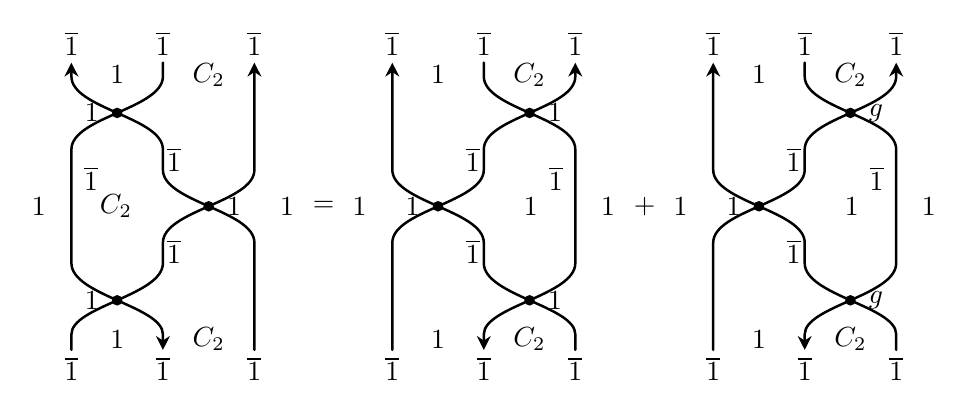
\begin{tikzpicture}[x=.83cm,y=.76cm]
\mixedThreeWires{arrowatend}{arrowatstart}{arrowatend}
\node[region] at (-0.5,2.4) {$1$};
\node[region] at (0.7,0.18) {$1$};
\node[region] at (2.1,0.18) {$C_2$};
\node[region] at (0.7,4.6) {$1$};
\node[region] at (2.1,4.6) {$C_2$};
\node[region] at (3.3,2.4) {$1$};
\node[strandlabel] at (0,-0.32) {$\overline{1}$};
\node[strandlabel] at (1.4,-0.32) {$\overline{1}$};
\node[strandlabel] at (2.8,-0.32) {$\overline{1}$};
\node[strandlabel] at (0,5.12) {$\overline{1}$};
\node[strandlabel] at (1.4,5.12) {$\overline{1}$};
\node[strandlabel] at (2.8,5.12) {$\overline{1}$};
\node[region] at (0.68,2.4) {$C_2$};
\fill (0.7,0.82875) circle (1.9pt);
\node[strandlabel,anchor=east] at (0.48,0.82875) {$1$};
\fill (2.1,2.4) circle (1.9pt);
\node[strandlabel,anchor=west] at (2.32,2.4) {$1$};
\fill (0.7,3.96) circle (1.9pt);
\node[strandlabel,anchor=east] at (0.48,3.96) {$1$};
\node[strandlabel,anchor=west] at (0.13,2.86) {$\overline{1}$};
\node[strandlabel,anchor=west] at (1.4,1.64) {$\overline{1}$};
\node[strandlabel,anchor=west] at (1.4,3.18) {$\overline{1}$};
\node at (3.86,2.4) {$=$};
\begin{scope}[shift={(4.91,0)}]
\begin{scope}[shift={(2.8,0)},xscale=-1]
\mixedThreeWires{arrowatend}{arrowatstart}{arrowatend}
\end{scope}
\node[region] at (-0.5,2.4) {$1$};
\node[region] at (0.7,0.18) {$1$};
\node[region] at (2.1,0.18) {$C_2$};
\node[region] at (0.7,4.6) {$1$};
\node[region] at (2.1,4.6) {$C_2$};
\node[region] at (3.3,2.4) {$1$};
\node[strandlabel] at (0,-0.32) {$\overline{1}$};
\node[strandlabel] at (1.4,-0.32) {$\overline{1}$};
\node[strandlabel] at (2.8,-0.32) {$\overline{1}$};
\node[strandlabel] at (0,5.12) {$\overline{1}$};
\node[strandlabel] at (1.4,5.12) {$\overline{1}$};
\node[strandlabel] at (2.8,5.12) {$\overline{1}$};
\node[region] at (2.12,2.4) {$1$};
\fill (2.1,0.82875) circle (1.9pt);
\node[strandlabel,anchor=west] at (2.32,0.82875) {$1$};
\fill (0.7,2.4) circle (1.9pt);
\node[strandlabel,anchor=east] at (0.48,2.4) {$1$};
\fill (2.1,3.96) circle (1.9pt);
\node[strandlabel,anchor=west] at (2.32,3.96) {$1$};
\node[strandlabel,anchor=east] at (2.67,2.86) {$\overline{1}$};
\node[strandlabel,anchor=east] at (1.4,1.64) {$\overline{1}$};
\node[strandlabel,anchor=east] at (1.4,3.18) {$\overline{1}$};
\end{scope}
\node at (8.77,2.4) {$+$};
\begin{scope}[shift={(9.82,0)}]
\begin{scope}[shift={(2.8,0)},xscale=-1]
\mixedThreeWires{arrowatend}{arrowatstart}{arrowatend}
\end{scope}
\node[region] at (-0.5,2.4) {$1$};
\node[region] at (0.7,0.18) {$1$};
\node[region] at (2.1,0.18) {$C_2$};
\node[region] at (0.7,4.6) {$1$};
\node[region] at (2.1,4.6) {$C_2$};
\node[region] at (3.3,2.4) {$1$};
\node[strandlabel] at (0,-0.32) {$\overline{1}$};
\node[strandlabel] at (1.4,-0.32) {$\overline{1}$};
\node[strandlabel] at (2.8,-0.32) {$\overline{1}$};
\node[strandlabel] at (0,5.12) {$\overline{1}$};
\node[strandlabel] at (1.4,5.12) {$\overline{1}$};
\node[strandlabel] at (2.8,5.12) {$\overline{1}$};
\node[region] at (2.12,2.4) {$1$};
\fill (2.1,0.82875) circle (1.9pt);
\node[strandlabel,anchor=west] at (2.32,0.82875) {$g$};
\fill (0.7,2.4) circle (1.9pt);
\node[strandlabel,anchor=east] at (0.48,2.4) {$1$};
\fill (2.1,3.96) circle (1.9pt);
\node[strandlabel,anchor=west] at (2.32,3.96) {$g$};
\node[strandlabel,anchor=east] at (2.67,2.86) {$\overline{1}$};
\node[strandlabel,anchor=east] at (1.4,1.64) {$\overline{1}$};
\node[strandlabel,anchor=east] at (1.4,3.18) {$\overline{1}$};
\end{scope}
\end{tikzpicture}
\end{center}
\end{example}


\begin{example}[An infinite expansion in Case 5]\label{ex:case-five-infinite-sum}
Take \(U=B=G=C=D=E\) infinite cyclic, written multiplicatively,
and \(A=F=1\). The left diagram with inclusions and unit labels sends
\([g,x]\mapsto gx\) after identifying the target with \(\C[U]\).
Its reverse cup has index \(1\). On the right \(B'=1\) is forced.
Each right diagram vanishes unless \(x\) is one of the finitely many
crossing elements of its first crossing. The same holds for a finite sum.
Using \(L,R\) for the drawings with this boundary, the pointwise
finite identity is
\[
 L(1,1,1)=\sum_{x\in U} R(x,x,1).
\]
The term indexed by \(x\) selects second coordinate \(x\) and sends
\([g,x]\) to \(gx\).

\begin{center}
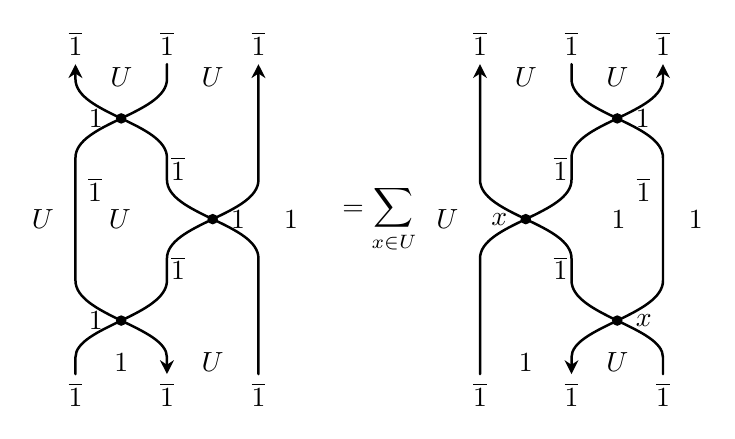
\begin{tikzpicture}[x=.83cm,y=.82cm]
\mixedThreeWires{arrowatend}{arrowatstart}{arrowatend}
\node[region] at (-0.5,2.4) {$U$};
\node[region] at (0.7,0.18) {$1$};
\node[region] at (2.1,0.18) {$U$};
\node[region] at (0.7,4.6) {$U$};
\node[region] at (2.1,4.6) {$U$};
\node[region] at (3.3,2.4) {$1$};
\node[strandlabel] at (0,-0.32) {$\overline{1}$};
\node[strandlabel] at (1.4,-0.32) {$\overline{1}$};
\node[strandlabel] at (2.8,-0.32) {$\overline{1}$};
\node[strandlabel] at (0,5.12) {$\overline{1}$};
\node[strandlabel] at (1.4,5.12) {$\overline{1}$};
\node[strandlabel] at (2.8,5.12) {$\overline{1}$};
\node[region] at (0.68,2.4) {$U$};
\fill (0.7,0.82875) circle (1.9pt);
\node[strandlabel,anchor=east] at (0.48,0.82875) {$1$};
\fill (2.1,2.4) circle (1.9pt);
\node[strandlabel,anchor=west] at (2.32,2.4) {$1$};
\fill (0.7,3.96) circle (1.9pt);
\node[strandlabel,anchor=east] at (0.48,3.96) {$1$};
\node[strandlabel,anchor=west] at (0.13,2.86) {$\overline{1}$};
\node[strandlabel,anchor=west] at (1.4,1.64) {$\overline{1}$};
\node[strandlabel,anchor=west] at (1.4,3.18) {$\overline{1}$};
\node at (4.65,2.4) {$=\displaystyle\sum_{x\in U}$};
\begin{scope}[shift={(6.19,0)}]
\begin{scope}[shift={(2.8,0)},xscale=-1]
\mixedThreeWires{arrowatend}{arrowatstart}{arrowatend}
\end{scope}
\node[region] at (-0.5,2.4) {$U$};
\node[region] at (0.7,0.18) {$1$};
\node[region] at (2.1,0.18) {$U$};
\node[region] at (0.7,4.6) {$U$};
\node[region] at (2.1,4.6) {$U$};
\node[region] at (3.3,2.4) {$1$};
\node[strandlabel] at (0,-0.32) {$\overline{1}$};
\node[strandlabel] at (1.4,-0.32) {$\overline{1}$};
\node[strandlabel] at (2.8,-0.32) {$\overline{1}$};
\node[strandlabel] at (0,5.12) {$\overline{1}$};
\node[strandlabel] at (1.4,5.12) {$\overline{1}$};
\node[strandlabel] at (2.8,5.12) {$\overline{1}$};
\node[region] at (2.12,2.4) {$1$};
\fill (2.1,0.82875) circle (1.9pt);
\node[strandlabel,anchor=west] at (2.32,0.82875) {$x$};
\fill (0.7,2.4) circle (1.9pt);
\node[strandlabel,anchor=east] at (0.48,2.4) {$x$};
\fill (2.1,3.96) circle (1.9pt);
\node[strandlabel,anchor=west] at (2.32,3.96) {$1$};
\node[strandlabel,anchor=east] at (2.67,2.86) {$\overline{1}$};
\node[strandlabel,anchor=east] at (1.4,1.64) {$\overline{1}$};
\node[strandlabel,anchor=east] at (1.4,3.18) {$\overline{1}$};
\end{scope}
\end{tikzpicture}
\end{center}
\end{example}


\subsubsection{Case 6. A right diagram can have no left replacement}


\begin{example}[A Case 6 projection with no left replacement]\label{ex:case-six-involution}
Use the boundary in Example~\ref{ex:case-five-two-terms}. The right diagram \(R(1,1,1)\)
fixes \(1\) and sends \(g\) to \(0\). On the left \(B=C_2\) is forced
since it receives \(D\) and \(E\) and lies in \(U=C_2\).
All embeddings of \(C_2\) are identities, so
\eqref{eq:three-left-middle-restriction} sends \(x\) to \(s^{-1}rxt\)
for each group-element triple. These maps and all their finite
linear combinations commute with translation by \(g\). The right
map sends \(g\) to zero, while translating
its value at \(1\) gives \(g\). Thus no finite sum of left diagrams
gives the right map. All cups in this example have index at most \(2\).

\begin{center}
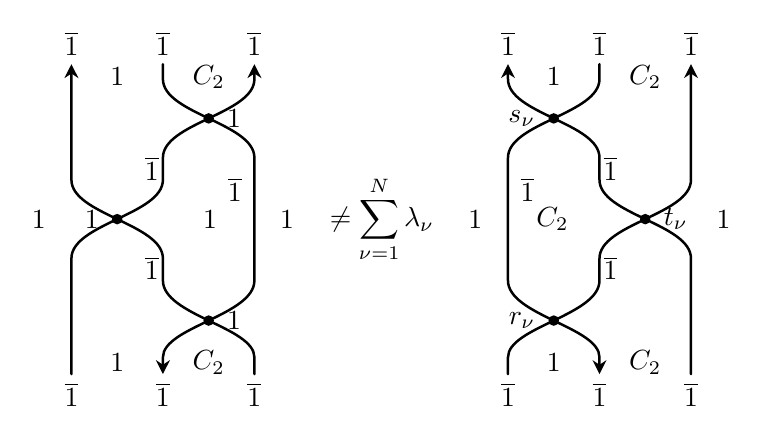
\begin{tikzpicture}[x=.83cm,y=.82cm]
\begin{scope}[shift={(2.8,0)},xscale=-1]
\mixedThreeWires{arrowatend}{arrowatstart}{arrowatend}
\end{scope}
\node[region] at (-0.5,2.4) {$1$};
\node[region] at (0.7,0.18) {$1$};
\node[region] at (2.1,0.18) {$C_2$};
\node[region] at (0.7,4.6) {$1$};
\node[region] at (2.1,4.6) {$C_2$};
\node[region] at (3.3,2.4) {$1$};
\node[strandlabel] at (0,-0.32) {$\overline{1}$};
\node[strandlabel] at (1.4,-0.32) {$\overline{1}$};
\node[strandlabel] at (2.8,-0.32) {$\overline{1}$};
\node[strandlabel] at (0,5.12) {$\overline{1}$};
\node[strandlabel] at (1.4,5.12) {$\overline{1}$};
\node[strandlabel] at (2.8,5.12) {$\overline{1}$};
\node[region] at (2.12,2.4) {$1$};
\fill (2.1,0.82875) circle (1.9pt);
\node[strandlabel,anchor=west] at (2.32,0.82875) {$1$};
\fill (0.7,2.4) circle (1.9pt);
\node[strandlabel,anchor=east] at (0.48,2.4) {$1$};
\fill (2.1,3.96) circle (1.9pt);
\node[strandlabel,anchor=west] at (2.32,3.96) {$1$};
\node[strandlabel,anchor=east] at (2.67,2.86) {$\overline{1}$};
\node[strandlabel,anchor=east] at (1.4,1.64) {$\overline{1}$};
\node[strandlabel,anchor=east] at (1.4,3.18) {$\overline{1}$};
\node at (4.75,2.4) {$\ne\displaystyle\sum_{\nu=1}^{N}\lambda_\nu$};
\begin{scope}[shift={(6.68,0)}]
\mixedThreeWires{arrowatend}{arrowatstart}{arrowatend}
\node[region] at (-0.5,2.4) {$1$};
\node[region] at (0.7,0.18) {$1$};
\node[region] at (2.1,0.18) {$C_2$};
\node[region] at (0.7,4.6) {$1$};
\node[region] at (2.1,4.6) {$C_2$};
\node[region] at (3.3,2.4) {$1$};
\node[strandlabel] at (0,-0.32) {$\overline{1}$};
\node[strandlabel] at (1.4,-0.32) {$\overline{1}$};
\node[strandlabel] at (2.8,-0.32) {$\overline{1}$};
\node[strandlabel] at (0,5.12) {$\overline{1}$};
\node[strandlabel] at (1.4,5.12) {$\overline{1}$};
\node[strandlabel] at (2.8,5.12) {$\overline{1}$};
\node[region] at (0.68,2.4) {$C_2$};
\fill (0.7,0.82875) circle (1.9pt);
\node[strandlabel,anchor=east] at (0.48,0.82875) {$r_\nu$};
\fill (2.1,2.4) circle (1.9pt);
\node[strandlabel,anchor=west] at (2.32,2.4) {$t_\nu$};
\fill (0.7,3.96) circle (1.9pt);
\node[strandlabel,anchor=east] at (0.48,3.96) {$s_\nu$};
\node[strandlabel,anchor=west] at (0.13,2.86) {$\overline{1}$};
\node[strandlabel,anchor=west] at (1.4,1.64) {$\overline{1}$};
\node[strandlabel,anchor=west] at (1.4,3.18) {$\overline{1}$};
\end{scope}
\end{tikzpicture}
\end{center}
\end{example}


\Needspace{12\baselineskip}
\section{Finite parabolic subgroups}\label{sec:finite-parabolic}

We compute conjugates, intersections, and subgroups generated by
unions of finite parabolics. Block counts give explicit double-coset
representatives and Mackey summands. The closure properties and the
Mackey formula give a bicategory of finite parabolic groups.

Let \(S_\infty\) be the group of finitely supported permutations of
\(\mathbb N\). A finite parabolic subgroup is a product
\(\prod_{i\in I}\operatorname{Sym}(X_i)\), where the \(X_i\) are pairwise
disjoint finite subsets of \(\mathbb N\) and \(I\) is finite. Each factor fixes the
complement of \(X_i\) pointwise. Omit empty blocks. The trivial group
is allowed. When comparing two such groups, take a finite set \(X\) containing both
unions of blocks and add singleton blocks so that both collections
partition \(X\).

\begin{proposition}[Closure of finite parabolics]\label{prop:parabolic-closure}
Finite parabolic subgroups are closed under conjugation in
\(S_\infty\), pairwise intersections, and forming the subgroup
generated by two of them.
\end{proposition}

\begin{proof}
\emph{Conjugation.}
If \(H=\prod_{i\in I}\operatorname{Sym}(X_i)\) and \(\alpha\in S_\infty\), then
\[
 \cg{\alpha}{H}=\prod_{i\in I}\operatorname{Sym}(\alpha(X_i)).
\]
Indeed, \((\alpha h\alpha^{-1})(\alpha(x))=\alpha(h(x))\) for \(x\in X_i\).
This preserves \(\alpha(X_i)\) for every \(h\in H\). Conversely, a
permutation preserving these images and fixing their complement
conjugates back to a permutation in \(H\).

\emph{Intersection.}
For \(A=\prod_{i\in I}\operatorname{Sym}(A_i)\) and
\(B=\prod_{j\in J}\operatorname{Sym}(B_j)\), use blocks that partition the same
finite set \(X\). A permutation of \(X\) preserves every \(A_i\) and
every \(B_j\) exactly when it preserves every \(A_i\cap B_j\).
Thus
\[
 A\cap B=\prod_{i\in I}\prod_{j\in J}\operatorname{Sym}(A_i\cap B_j),
\]
where empty intersections contribute trivial factors.

\emph{Subgroup generated by a union.}
Join \(A_i\) to \(B_j\) in a graph whenever \(A_i\cap B_j\ne\varnothing\).
For each connected component, let \(\widetilde{AB}^{(k)}\) be the
union of its blocks. Each point lies in an \(A\)-block and a \(B\)-block
joined by an edge, so either side gives the same union. The components give the
minimal nonempty collections of blocks on the two sides with a
common union, since any such collection contains every neighbor of
each selected block.

Both \(A\) and \(B\) preserve each \(\widetilde{AB}^{(k)}\). Inside \(\widetilde{AB}^{(k)}\), a path of
overlapping blocks joins any two points. Choosing a point in each
overlap gives a chain whose consecutive transpositions belong to
\(A\) or \(B\). After removing repetitions, successive applications of
\((x\,z)=(y\,z)(x\,y)(y\,z)\) give the transposition of the endpoints.
Since transpositions generate each symmetric group, the join is
\(\langle A\cup B\rangle=\prod_k\operatorname{Sym}(\widetilde{AB}^{(k)})\).
\end{proof}

\begin{lemma}[Parabolic subgroups below and above a finite group]\label{lem:extremal-parabolics}
Let \(P\le S_\infty\) be finite. Its largest parabolic subgroup is
generated by all transpositions in \(P\). Its smallest parabolic
overgroup is the product of the symmetric groups on its
nonsingleton orbits.
\end{lemma}

\begin{proof}
Each transposition in \(P\) generates a parabolic subgroup. Their
join is parabolic by Proposition~\ref{prop:parabolic-closure} and
lies in \(P\). Every parabolic subgroup of \(P\) is generated by
transpositions in \(P\), giving maximality.
For the overgroup, \(P\) acts on a finite set containing the supports
of its elements and preserves every orbit on it. The product on
the nonsingleton orbits contains \(P\). Each block of any parabolic
overgroup of \(P\) is preserved by \(P\), so each orbit lies in one
block. The stated product therefore lies in every parabolic overgroup.
\end{proof}

\subsection{Examples}


\begin{example}[Conjugation, intersection, and generation]\label{ex:parabolic-block-operations}
Take
\[
 \begin{aligned}
 A&=\operatorname{Sym}(\{1,2,3\})\times\operatorname{Sym}(\{4,5\}),\\
 B&=\operatorname{Sym}(\{2,3,4\})\times\operatorname{Sym}(\{6,7\}).
 \end{aligned}
\]
Use singleton blocks for the remaining points in \(\{1,\ldots,7\}\).

\emph{Conjugation.} For \(\alpha=(1\,4\,6)\), the two nonsingleton
blocks of \(A\) map to \(\{2,3,4\}\) and \(\{5,6\}\), so
\[
 \cg{\alpha}{A}=
 \operatorname{Sym}(\{2,3,4\})\times\operatorname{Sym}(\{5,6\}).
\]

\emph{Intersection.} The only intersection of blocks with at least
two points is \(\{1,2,3\}\cap\{2,3,4\}=\{2,3\}\). Hence
\(A\cap B=\operatorname{Sym}(\{2,3\})\).

\emph{Subgroup generated by a union.} The block \(\{2,3,4\}\)
overlaps both nonsingleton blocks of \(A\), so their common union
is \(\{1,2,3,4,5\}\). The block \(\{6,7\}\) meets only its two
singleton blocks on the \(A\) side. Thus
\[
 \langle A\cup B\rangle
 =\operatorname{Sym}(\{1,2,3,4,5\})\times\operatorname{Sym}(\{6,7\}).
\]
For instance, the join contains \((1\,5)\), obtained by taking
endpoint transpositions along a path of overlapping blocks.
\end{example}

\subsection{Double cosets from tableaux}\label{sec:parabolic-double-cosets}

First let \(G=\operatorname{Sym}(X)\). Write \(K=\prod_i\operatorname{Sym}(X_i)\)
and \(H=\prod_j\operatorname{Sym}(Y_j)\), with singleton blocks added so that
both partitions cover \(X\). Order each list of blocks and order the points
within each block by their natural order in \(\mathbb N\).

Make a tableau whose \(i\)-th row has positions labeled by the points of
\(X_i\). In the initial tableau \(t_0\), the box at position \(x\) has
entry \(j\) if \(x\in Y_j\). A permutation \(\sigma\in G\) sends the
entry at \(x\) to position \(\sigma(x)\). Write \(R_{ij}\) for the number
of entries \(j\) in row \(i\) of \(\sigma t_0\).

The classification is due to James and Kerber \cite[Thm.~1.3.10]{james-kerber}.

\begin{proposition}[Double coset representatives]\label{prop:parabolic-double-cosets}
The map
\[
 K\sigma H\longmapsto (R_{ij}),
 \qquad R_{ij}=|X_i\cap\sigma(Y_j)|
\]
is a bijection onto the nonnegative integer matrices with row sums
\(|X_i|\) and column sums \(|Y_j|\). For a given matrix, construct
a representative as follows.
\end{proposition}

\begin{enumerate}
\item Split the ordered block \(X_i\) into consecutive pieces of sizes
\(R_{i1},R_{i2},\ldots\). The \(j\)-th piece consists of the positions
that will carry entry \(j\).
\item Split the ordered block \(Y_j\) into consecutive pieces of sizes
\(R_{1j},R_{2j},\ldots\). Map its \(i\)-th piece in order to the
\(j\)-th piece of \(X_i\).
\end{enumerate}

The matched pieces partition \(X\) on each side, so the prescribed
maps give a permutation. It sends exactly \(R_{ij}\) points from
\(Y_j\) into \(X_i\).

For any representative \(\sigma\), the Mackey intersection is
\[
 K\cap\sigma H\sigma^{-1}
   =\prod_{i,j}\operatorname{Sym}(X_i\cap\sigma(Y_j)).
\]
This is the block-intersection formula of
Proposition~\ref{prop:parabolic-closure} applied to \(K\) and
\(\sigma H\sigma^{-1}\).


\begin{example}[A double-coset representative from a tableau]\label{ex:tableau-s6}
In \(S_6\) use the two subgroups
\[
\begin{aligned}
K&=\operatorname{Sym}(\{1,2,4,5\})\times\operatorname{Sym}(\{3,6\}),\\
H&=\operatorname{Sym}(\{1,3,5\})\times\operatorname{Sym}(\{2,4,6\}).
\end{aligned}
\]
For the matrix \(\left(\begin{smallmatrix}1&3\\2&0\end{smallmatrix}\right)\),
the first row receives one \(1\) at position \(1\). The second row
receives two \(1\)'s at positions \(3,6\). The ordered matching
gives \(\sigma=(5\,6)\), and its Mackey group is
\(\operatorname{Sym}(\{2,4,5\})\times\operatorname{Sym}(\{3,6\})\).
\end{example}


\begin{example}[One-sided coset representatives]\label{ex:tableau-one-sided}
Taking \(H=1\), with each \(Y_j\) a singleton, gives representatives
for the right cosets \(K\sigma\). Their inverses give representatives
for the left cosets \(\sigma^{-1}K\).
\end{example}

\subsection{Two blocks and products}\label{sec:parabolic-binary-cosets}

When \(K\) and \(H\) each have two blocks in \(\operatorname{Sym}(X)\),
write \(n=|X|\), \(c=|X_1|\), and \(d=|Y_1|\). The matrices are precisely
\[
 \begin{pmatrix}
 a&c-a\\ d-a&n-c-d+a
 \end{pmatrix},
 \qquad \max(0,c+d-n)\le a\le\min(c,d),\qquad a\in\mathbb Z.
\]
The entry \(a\) determines the other three entries, and the bounds
make all four entries nonnegative.

For standard two-block subgroups of \(S_n\), take
\(K=S_{n_1}\times S_{n-n_1}\) and \(H=S_{n_2}\times S_{n-n_2}\),
where \(1\le n_1,n_2<n\) and each first block begins at \(1\).
An alternative
set of representatives, convenient for computing the intersections,
is
\[
 \begin{gathered}
 m=\min(n_1,n_2,n-\max(n_1,n_2)),\qquad \sigma_0=1,\\
 \sigma_i=(\min(n_1,n_2)-i+1,\ \max(n_1,n_2)+i)\,\sigma_{i-1}
     \qquad (1\le i\le m).
 \end{gathered}
\]
The transpositions are disjoint. Each one takes a further point
of \(Y_1\) out of \(X_1\) and puts a point of its complement in
\(X_1\). Thus \(a_i=\min(n_1,n_2)-i\) takes every allowed value
exactly once. The four Mackey block sizes, in row order, are
\[
 a_i,\qquad n_1-a_i,\qquad n_2-a_i,\qquad n-n_1-n_2+a_i.
\]
The four intersections are intervals in the standard order, with
empty intervals omitted.

\begin{example}[Equal two-block subgroups]\label{ex:equal-two-blocks}
For
\(K=H=S_n\times S_m\le S_{n+m}\), \(n\ge m\), the representatives
swap the last \(i\) points of the first block with the first
\(i\) points of the second block in reverse order. The intersection
group is \(S_{n-i}\times S_i\times S_i\times S_{m-i}\),
with a zero-size factor interpreted as the trivial group.
\end{example}


\begin{example}[Conjugation exchanging two factors]\label{ex:two-block-factor-exchange}
Even when \(\sigma_i^{-1}L_i\sigma_i=L_i\), the conjugation can
exchange factors. For \(n=m=2\), the representative with \(i=2\)
exchanges the two \(S_2\) factors.
\end{example}

Now let \(G=\prod_i G_i\) be a finite parabolic group.
On the finite set partitioned by the blocks of \(G\), each block
of \(K\) or \(H\) lies inside a block of \(G\), since every
transposition within it belongs to \(G\). Thus
\(K=\prod_i K_i\), \(H=\prod_i H_i\), where \(K_i,H_i\le G_i\)
are the restrictions to that block. Double coset equality is
componentwise, giving
\[
 K\backslash G/H \cong \prod_i K_i\backslash G_i/H_i .
\]
Choose one matrix and its representative in each \(G_i\) and
multiply those representatives, whose supports are disjoint.
This gives every double coset once. A factor with \(K_i=G_i\)
or \(H_i=G_i\) contributes only the representative \(1\).


\begin{example}[A product with one double coset]\label{ex:product-two-factors}
For \(G=S_4\times S_4\), \(K=(S_2\times S_2)\times S_4\) and
\(H=S_4\times(S_2\times S_2)\), each ambient block contributes
one double coset. The representative is \(1\), and
\(K\cap H=S_2^4\).
\end{example}


\begin{example}[A product with three double cosets]\label{ex:product-three-factors}
For \(G=S_4^3\) on three successive blocks,
\(K=(S_2\times S_2)\times S_4\times(S_2\times S_2)\) and
\(H=S_4\times(S_2\times S_2)\times(S_2\times S_2)\), the first
two blocks again contribute \(1\). In the last block choose
\(\sigma_0=1\), \(\sigma_1=(10\,11)\), and
\(\sigma_2=(9\,12)(10\,11)\). The Mackey groups are
\(L_0=L_2=S_2^6\) and \(L_1=S_2^4\). Conjugation by \(\sigma_2\)
exchanges the last two \(S_2\) factors of \(L_2\).
\end{example}

A Mackey group refines both block partitions, with the \(H\)
partition transported by the representative. A binary split on
each side can yield four blocks inside a single block of \(G\).


\begin{example}[A two-block split giving four intersections]\label{ex:four-intersections}
The middle double coset of
\(S_2\times S_2\backslash S_4/(S_2\times S_2)\) has four
singleton blocks. Thus the family of binary refinements of \(G\)
with a prescribed split size need not contain the Mackey groups.
\end{example}

\Needspace{22\baselineskip}
\subsection{Mackey decomposition for finite parabolics}
\label{sec:mackey-finite-parabolic}

\begin{theorem}[Mackey decomposition with explicit parabolic representatives]
\label{thm:mackey-finite-parabolic}
Let \(K,H,G\) be finite parabolics in \(S_\infty\), and let
\(\cg{\alpha}{K},\cg{\beta}{H}\le G\). Index the double cosets
\[
 J=(\cg{\alpha}{K})\backslash G/(\cg{\beta}{H}),
 \qquad
 G=\bigsqcup_{j\in J}(\cg{\alpha}{K})\sigma_j(\cg{\beta}{H})
\]
by the tuples of matrices for the blocks of \(G\), with
\(\sigma_j\) obtained by the ordered matching of
Proposition~\ref{prop:parabolic-double-cosets}. Put
\[
 L_j=\cg{\alpha}{K}\cap\cg{\sigma_j\beta}{H},
 \qquad
 \lambda_j(\ell)=\alpha^{-1}\ell\alpha,\qquad
 \mu_j(\ell)=\beta^{-1}\sigma_j^{-1}\ell\sigma_j\beta .
\]
Then \(L_j\) is the product of the symmetric groups on the
corresponding block intersections, and there is a natural
isomorphism
\[
 \Res_{\alpha_*}\circ\Ind_{\beta_*}
   \cong\bigoplus_{j\in J}\Ind_{\lambda_j}\circ\Res_{\mu_j}.
\]
For inclusion boundary embeddings this is
\[
 \Res_K^G\circ\Ind_H^G
 \cong \bigoplus_{j\in K\backslash G/H}
   \Ind_{L_j}^K\circ c_{\sigma_j}\circ
   \Res_{\sigma_j^{-1}L_j\sigma_j}^{H},
\]
where \(c_{\sigma_j}\) gives \(\ell\in L_j\) the action of
\(\sigma_j^{-1}\ell\sigma_j\).
\end{theorem}

\begin{proof}
Conjugation preserves the parabolic subgroups. The ordered matching
in each block of \(G\) gives the double cosets, and the
block-intersection formula computes \(L_j\). Apply
Theorem~\ref{thm:mackey} to these representatives, using the two
displayed embeddings of \(L_j\). For inclusions,
\(\mu_j\) is conjugation by \(\sigma_j^{-1}\) into its image
followed by inclusion in \(H\), giving the stated factorization
of restriction.
\end{proof}

\subsection{The finite-parabolic bimodule bicategory}
\label{sec:parabolic-bicategory}

Khovanov considers a bicategory generated by induction and restriction
between finite groups \cite[\S~3.2]{khovanov}. The closure and Mackey
results above give a version for finite parabolics with one intermediate
group per summand.

\begin{corollary}[The finite-parabolic bimodule bicategory]
\label{cor:parabolic-bicategory}
Finite parabolic subgroups of \(S_\infty\) form a bicategory with
1-morphisms \(H\to K\) the bimodules isomorphic to finite direct sums of
\[
 \C[K]\otimes_{\C[L]}\C[H],
 \qquad K\xleftarrow{a}L\xrightarrow{b}H,
\]
where \(L\) is finite parabolic and \(a,b\) are conjugation embeddings
in \(S_\infty\). The 2-morphisms are bimodule maps. Composition is
tensor product over the group algebra of the common group.
\end{corollary}

\begin{proof}
With either leg the identity, the displayed bimodule is an induction
or restriction strand. With both legs the identity at \(H\), it is
the regular bimodule \(\C[H]\).

For composition with \(H\xleftarrow{c}M\xrightarrow{d}J\), apply
Theorem~\ref{thm:mackey-finite-parabolic} to the middle factor
\(\C[H]\) with its actions through \(b\) and \(c\). For each
representative \(r\in H\) of a double coset in \(b(L)\backslash H/c(M)\),
the resulting summand has middle group
\[
 b(L)\cap r c(M)r^{-1}
\]
and embeddings \(x\mapsto a(b^{-1}(x))\) into \(K\) and
\(x\mapsto d(c^{-1}(r^{-1}xr))\) into \(J\). These are conjugation
embeddings, and the middle group is finite parabolic by
Proposition~\ref{prop:parabolic-closure}. Theorem~\ref{thm:mackey-finite-parabolic}
also gives explicit representatives \(r\) by ordered matching on
the blocks of \(H\). There are finitely many double cosets, and tensor
product distributes over finite direct sums. The associativity and
unit isomorphisms are those of bimodule tensor product.
\end{proof}

Proposition~\ref{prop:parabolic-closure} also gives a least parabolic
group containing any finite collection of parabolic images. It is the
subgroup generated by their union, called their join. If all the
images lie in a prescribed group, so does their join.
Section~\ref{sec:parabolic-moves} uses joins to construct common
internal regions for Reidemeister moves.

\Needspace{12\baselineskip}
\section{Reidemeister identities for finite parabolics}\label{sec:parabolic-moves}

We apply the block computations to the three types of Reidemeister
moves. They give curl coefficients, common internal groups for
two crossings, and explicit choices or obstructions for
three-crossing replacements, including their multiplicities over
general coefficient rings.

We work in the bicategory of Section~\ref{sec:parabolic-bicategory},
with \(U=S_\infty\) and all region groups finite parabolic. We use the
diagrams and labels of
Sections~\ref{sec:reidemeister-one}--\ref{sec:reidemeister-three}.

\subsection{Reidemeister I}

\begin{proposition}[Curls from block refinements]\label{prop:parabolic-curls}
In Theorem~\ref{thm:reidemeister-one}, write
\(H=\prod_{i\in I}\operatorname{Sym}(X_i)\) and
\(\cg{\delta}{K}=\prod_{j\in J}\operatorname{Sym}(Y_j)\), using
singleton blocks to partition the same finite set. The right up-curl
and left down-curl have scalar
\[
 [H:\cg{\delta}{K}]
 =\prod_{i\in I}\frac{|X_i|!}{\prod_{j:Y_j\subseteq X_i}|Y_j|!}.
\]
Merging two blocks of sizes \(a,b\) gives a scalar
\(\binom{a+b}{a}\). A sequence of such merges factors the curl through
the intermediate parabolics, and the product of its scalars is
independent of the merge order. The other two curls have scalar \(1\).
\end{proposition}

\begin{proof}
A transposition of two points of \(Y_j\) belongs to \(H\), so both
points lie in the same \(X_i\). Thus the \(Y_j\) refine the \(X_i\),
including the singleton blocks.
The index formula follows by dividing the orders of the block
factors. A single merge replaces \(a!b!\) by \((a+b)!\).

For the factorization diagram use the image \(A=\cg{\delta}{K}\)
as the internal group and the inclusion into \(H\).
To factor the curl through an intermediate group
\(\cg{\delta}{K}\le B\le H\), choose representatives \(r\) of the right
cosets of \(\cg{\delta}{K}\) in \(B\) and \(t\) of the right cosets
of \(B\) in \(H\). The products \(rt\) represent the right cosets
of \(\cg{\delta}{K}\) in \(H\) exactly once. In the up-curl calculation
the cup and cap then contribute
\[
 \sum_t\sum_r x\,\alpha_*(t^{-1})\alpha_*(r^{-1})
                    \alpha_*(r)\alpha_*(t).
\]
The sum over \(r\) is the inner curl and contributes
\([B:\cg{\delta}{K}]\). The outer cup and cap contribute \([H:B]\).
In the down-curl the same product of factors acts on the left of \(x\).
Iterating gives the asserted factorization. Every sequence of binary
merges within the \(X_i\) has the same total index. The two curls
enclosing \(G\) are the identities of
Theorem~\ref{thm:reidemeister-one}.
\end{proof}

\begin{center}
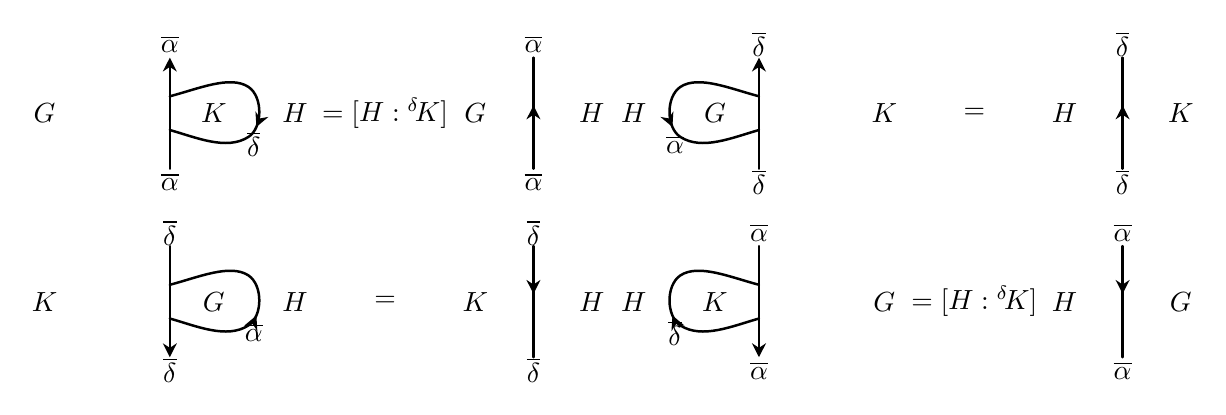
\begin{tikzpicture}[x=.86cm,y=.63cm]
\begin{scope}[shift={(-3.28,1.90)}]
\begin{scope}[xscale=1]
\draw[arrowatend] (0,-1.12)--(0,1.12);
\draw[oriented] (0,.34)
    .. controls (.42,.49) and (.89,.77) .. (1.16,.53)
    .. controls (1.38,.33) and (1.37,-.30) .. (1.16,-.48)
    .. controls (.84,-.76) and (.39,-.49) .. (0,-.34);
\node[region] at (.65,0) {$K$};
\node[strandlabel] at (1.24,-.63) {$\overline{\delta}$};
\end{scope}
\node[region] at (-1.85,0) {$G$};
\node[region] at (1.85,0) {$H$};
\node[strandlabel] at (0,-1.39) {$\overline{\alpha}$};
\node[strandlabel] at (0,1.39) {$\overline{\alpha}$};
\end{scope}
\node at (-0.09999999999999964,1.90) {$=[H:{}^\delta\!K]$};
\begin{scope}[shift={(2.0900000000000003,1.90)}]
\draw[oriented] (0,-1.12)--(0,1.12);
\node[region] at (-0.86,0) {$G$};
\node[region] at (0.86,0) {$H$};
\node[strandlabel] at (0,-1.39) {$\overline{\alpha}$};
\node[strandlabel] at (0,1.39) {$\overline{\alpha}$};
\end{scope}
\begin{scope}[shift={(-3.28,-1.90)}]
\begin{scope}[xscale=1]
\draw[arrowatstart] (0,-1.12)--(0,1.12);
\draw[reverseoriented] (0,.34)
    .. controls (.42,.49) and (.89,.77) .. (1.16,.53)
    .. controls (1.38,.33) and (1.37,-.30) .. (1.16,-.48)
    .. controls (.84,-.76) and (.39,-.49) .. (0,-.34);
\node[region] at (.65,0) {$G$};
\node[strandlabel] at (1.24,-.63) {$\overline{\alpha}$};
\end{scope}
\node[region] at (-1.85,0) {$K$};
\node[region] at (1.85,0) {$H$};
\node[strandlabel] at (0,-1.39) {$\overline{\delta}$};
\node[strandlabel] at (0,1.39) {$\overline{\delta}$};
\end{scope}
\node at (-0.09999999999999964,-1.90) {$=$};
\begin{scope}[shift={(2.0900000000000003,-1.90)}]
\draw[reverseoriented] (0,-1.12)--(0,1.12);
\node[region] at (-0.86,0) {$K$};
\node[region] at (0.86,0) {$H$};
\node[strandlabel] at (0,-1.39) {$\overline{\delta}$};
\node[strandlabel] at (0,1.39) {$\overline{\delta}$};
\end{scope}
\begin{scope}[shift={(5.42,1.90)}]
\begin{scope}[xscale=-1]
\draw[arrowatend] (0,-1.12)--(0,1.12);
\draw[oriented] (0,.34)
    .. controls (.42,.49) and (.89,.77) .. (1.16,.53)
    .. controls (1.38,.33) and (1.37,-.30) .. (1.16,-.48)
    .. controls (.84,-.76) and (.39,-.49) .. (0,-.34);
\node[region] at (.65,0) {$G$};
\node[strandlabel] at (1.24,-.63) {$\overline{\alpha}$};
\end{scope}
\node[region] at (-1.85,0) {$H$};
\node[region] at (1.85,0) {$K$};
\node[strandlabel] at (0,-1.39) {$\overline{\delta}$};
\node[strandlabel] at (0,1.39) {$\overline{\delta}$};
\end{scope}
\node at (8.60,1.90) {$=$};
\begin{scope}[shift={(10.79,1.90)}]
\draw[oriented] (0,-1.12)--(0,1.12);
\node[region] at (-0.86,0) {$H$};
\node[region] at (0.86,0) {$K$};
\node[strandlabel] at (0,-1.39) {$\overline{\delta}$};
\node[strandlabel] at (0,1.39) {$\overline{\delta}$};
\end{scope}
\begin{scope}[shift={(5.42,-1.90)}]
\begin{scope}[xscale=-1]
\draw[arrowatstart] (0,-1.12)--(0,1.12);
\draw[reverseoriented] (0,.34)
    .. controls (.42,.49) and (.89,.77) .. (1.16,.53)
    .. controls (1.38,.33) and (1.37,-.30) .. (1.16,-.48)
    .. controls (.84,-.76) and (.39,-.49) .. (0,-.34);
\node[region] at (.65,0) {$K$};
\node[strandlabel] at (1.24,-.63) {$\overline{\delta}$};
\end{scope}
\node[region] at (-1.85,0) {$H$};
\node[region] at (1.85,0) {$G$};
\node[strandlabel] at (0,-1.39) {$\overline{\alpha}$};
\node[strandlabel] at (0,1.39) {$\overline{\alpha}$};
\end{scope}
\node at (8.60,-1.90) {$=[H:{}^\delta\!K]$};
\begin{scope}[shift={(10.79,-1.90)}]
\draw[reverseoriented] (0,-1.12)--(0,1.12);
\node[region] at (-0.86,0) {$H$};
\node[region] at (0.86,0) {$G$};
\node[strandlabel] at (0,-1.39) {$\overline{\alpha}$};
\node[strandlabel] at (0,1.39) {$\overline{\alpha}$};
\end{scope}
\end{tikzpicture}
\end{center}

\begin{center}
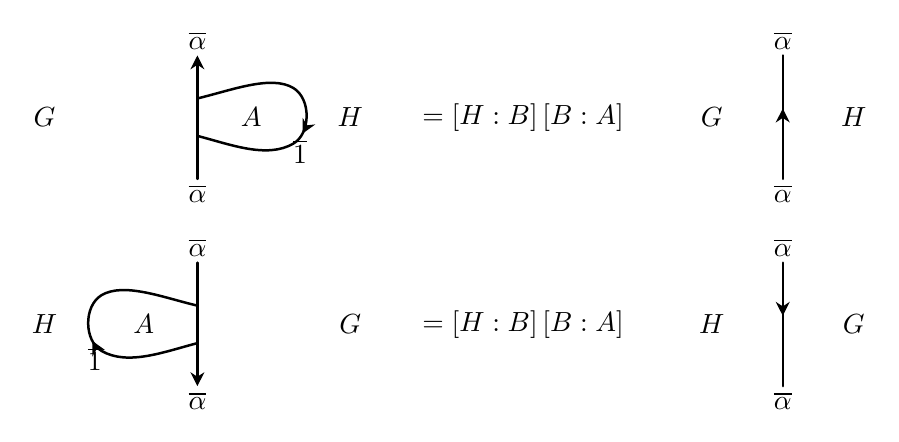
\begin{tikzpicture}[x=1.05cm,y=.7cm]
\begin{scope}[shift={(0,1.88)}]
\begin{scope}[xscale=1]
\draw[arrowatend] (0,-1.12)--(0,1.12);
\draw[oriented] (0,.34)
    .. controls (.42,.49) and (.89,.77) .. (1.16,.53)
    .. controls (1.38,.33) and (1.37,-.30) .. (1.16,-.48)
    .. controls (.84,-.76) and (.39,-.49) .. (0,-.34);
\node[region] at (.65,0) {$A$};
\node[strandlabel] at (1.24,-.63) {$\overline{1}$};
\end{scope}
\node[region] at (-1.85,0) {$G$};
\node[region] at (1.85,0) {$H$};
\node[strandlabel] at (0,-1.39) {$\overline{\alpha}$};
\node[strandlabel] at (0,1.39) {$\overline{\alpha}$};
\end{scope}
\node at (3.94,1.88) {$=[H:B]\,[B:A]$};
\begin{scope}[shift={(7.08,1.88)}]
\draw[oriented] (0,-1.12)--(0,1.12);
\node[region] at (-0.86,0) {$G$};
\node[region] at (0.86,0) {$H$};
\node[strandlabel] at (0,-1.39) {$\overline{\alpha}$};
\node[strandlabel] at (0,1.39) {$\overline{\alpha}$};
\end{scope}
\begin{scope}[shift={(0,-1.88)}]
\begin{scope}[xscale=-1]
\draw[arrowatstart] (0,-1.12)--(0,1.12);
\draw[reverseoriented] (0,.34)
    .. controls (.42,.49) and (.89,.77) .. (1.16,.53)
    .. controls (1.38,.33) and (1.37,-.30) .. (1.16,-.48)
    .. controls (.84,-.76) and (.39,-.49) .. (0,-.34);
\node[region] at (.65,0) {$A$};
\node[strandlabel] at (1.24,-.63) {$\overline{1}$};
\end{scope}
\node[region] at (-1.85,0) {$H$};
\node[region] at (1.85,0) {$G$};
\node[strandlabel] at (0,-1.39) {$\overline{\alpha}$};
\node[strandlabel] at (0,1.39) {$\overline{\alpha}$};
\end{scope}
\node at (3.94,-1.88) {$=[H:B]\,[B:A]$};
\begin{scope}[shift={(7.08,-1.88)}]
\draw[reverseoriented] (0,-1.12)--(0,1.12);
\node[region] at (-0.86,0) {$H$};
\node[region] at (0.86,0) {$G$};
\node[strandlabel] at (0,-1.39) {$\overline{\alpha}$};
\node[strandlabel] at (0,1.39) {$\overline{\alpha}$};
\end{scope}
\end{tikzpicture}
\end{center}

\begin{proposition}[Curls for a join and an intersection]\label{prop:parabolic-curl-join}
Fix either of the two index-valued curls on a strand and let \(c_A\)
denote that curl with internal group \(A\le H\), using inclusions into
\(H\). For finite parabolics \(A,B\le H\),
\[
 c_{A\cap B}\circ c_{\langle A\cup B\rangle}
  =\frac{|AB|}{|\langle A\cup B\rangle|}\,(c_A\circ c_B).
\]
The scalar is \(1\) exactly when, on each block of
\(\langle A\cup B\rangle\), at least one of the two original
partitions has that whole block.
\end{proposition}

\begin{proof}
The block groups on both sides are allowed by
Proposition~\ref{prop:parabolic-closure}. Apply
Theorem~\ref{thm:reidemeister-one} and use
\(|AB|=|A||B|/|A\cap B|\), where \(AB\) is the set of products \(ab\).
The scalar is \(1\) exactly when this set is the whole join.
The product set splits over the blocks of the join. On a block where
one partition has a single part, its symmetric group is already
the whole factor. If both partitions split the block, choose two
points in different \(B\)-parts and a permutation sending them
to points in different \(A\)-parts. Swapping the two images changes
the size of an intersection of an \(A\)-part with an image of a
\(B\)-part. These sizes are constant on an \(A,B\) double coset,
so there is more than one double coset on that block. Then \(AB\)
cannot be the whole factor.
\end{proof}


\begin{example}[Unequal products of curls]\label{ex:curl-join-s3}
For \(H=\operatorname{Sym}(\{1,2,3\})\), \(A=\langle(12)\rangle\)
and \(B=\langle(23)\rangle\), the intersection is trivial and the
join is \(H\). Write \(J=\langle A\cup B\rangle\) in the diagram.
The two products of curls have scalars \(6\) and \(9\),
respectively.

\begin{center}
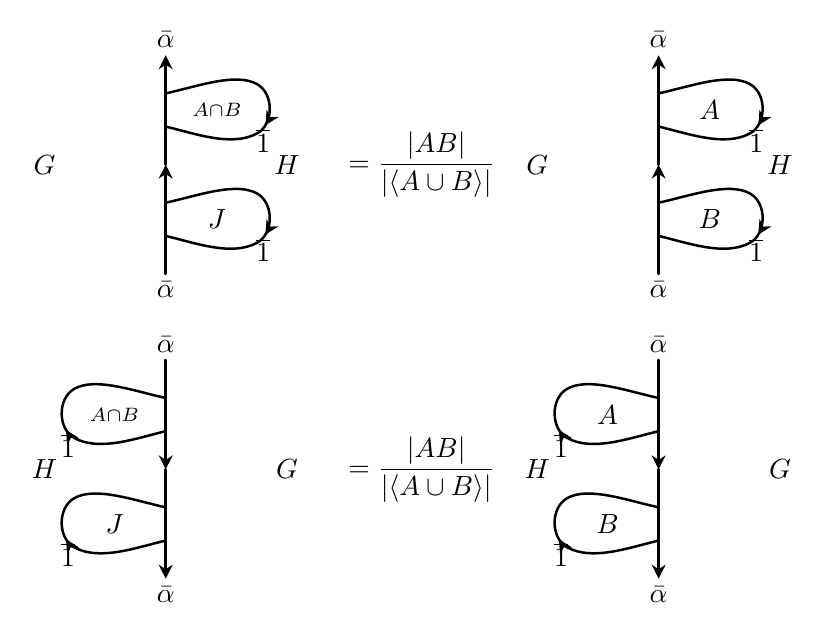
\begin{tikzpicture}[x=1cm,y=.62cm]
\begin{scope}[shift={(0,3.12)}]
\begin{scope}[shift={(0,-1.12)}]
\begin{scope}[xscale=1]
\draw[arrowatend] (0,-1.12)--(0,1.12);
\draw[oriented] (0,.34)
    .. controls (.42,.49) and (.89,.77) .. (1.16,.53)
    .. controls (1.38,.33) and (1.37,-.30) .. (1.16,-.48)
    .. controls (.84,-.76) and (.39,-.49) .. (0,-.34);
\node[region] at (.65,0) {$J$};
\node[strandlabel] at (1.24,-.63) {$\overline{1}$};
\end{scope}
\end{scope}
\begin{scope}[shift={(0,1.12)}]
\begin{scope}[xscale=1]
\draw[arrowatend] (0,-1.12)--(0,1.12);
\draw[oriented] (0,.34)
    .. controls (.42,.49) and (.89,.77) .. (1.16,.53)
    .. controls (1.38,.33) and (1.37,-.30) .. (1.16,-.48)
    .. controls (.84,-.76) and (.39,-.49) .. (0,-.34);
\node[region] at (.65,0) {$\scriptstyle A\cap B$};
\node[strandlabel] at (1.24,-.63) {$\overline{1}$};
\end{scope}
\end{scope}
\node[region] at (-1.54,0) {$G$};
\node[region] at (1.54,0) {$H$};
\node[strandlabel] at (0,-2.56) {$\bar\alpha$};
\node[strandlabel] at (0,2.56) {$\bar\alpha$};
\end{scope}
\node at (3.25,3.12) {$=\dfrac{|AB|}{|\langle A\cup B\rangle|}$};
\begin{scope}[shift={(6.26,3.12)}]
\begin{scope}[shift={(0,-1.12)}]
\begin{scope}[xscale=1]
\draw[arrowatend] (0,-1.12)--(0,1.12);
\draw[oriented] (0,.34)
    .. controls (.42,.49) and (.89,.77) .. (1.16,.53)
    .. controls (1.38,.33) and (1.37,-.30) .. (1.16,-.48)
    .. controls (.84,-.76) and (.39,-.49) .. (0,-.34);
\node[region] at (.65,0) {$B$};
\node[strandlabel] at (1.24,-.63) {$\overline{1}$};
\end{scope}
\end{scope}
\begin{scope}[shift={(0,1.12)}]
\begin{scope}[xscale=1]
\draw[arrowatend] (0,-1.12)--(0,1.12);
\draw[oriented] (0,.34)
    .. controls (.42,.49) and (.89,.77) .. (1.16,.53)
    .. controls (1.38,.33) and (1.37,-.30) .. (1.16,-.48)
    .. controls (.84,-.76) and (.39,-.49) .. (0,-.34);
\node[region] at (.65,0) {$A$};
\node[strandlabel] at (1.24,-.63) {$\overline{1}$};
\end{scope}
\end{scope}
\node[region] at (-1.54,0) {$G$};
\node[region] at (1.54,0) {$H$};
\node[strandlabel] at (0,-2.56) {$\bar\alpha$};
\node[strandlabel] at (0,2.56) {$\bar\alpha$};
\end{scope}
\begin{scope}[shift={(0,-3.12)}]
\begin{scope}[shift={(0,-1.12)}]
\begin{scope}[xscale=-1]
\draw[arrowatstart] (0,-1.12)--(0,1.12);
\draw[reverseoriented] (0,.34)
    .. controls (.42,.49) and (.89,.77) .. (1.16,.53)
    .. controls (1.38,.33) and (1.37,-.30) .. (1.16,-.48)
    .. controls (.84,-.76) and (.39,-.49) .. (0,-.34);
\node[region] at (.65,0) {$J$};
\node[strandlabel] at (1.24,-.63) {$\overline{1}$};
\end{scope}
\end{scope}
\begin{scope}[shift={(0,1.12)}]
\begin{scope}[xscale=-1]
\draw[arrowatstart] (0,-1.12)--(0,1.12);
\draw[reverseoriented] (0,.34)
    .. controls (.42,.49) and (.89,.77) .. (1.16,.53)
    .. controls (1.38,.33) and (1.37,-.30) .. (1.16,-.48)
    .. controls (.84,-.76) and (.39,-.49) .. (0,-.34);
\node[region] at (.65,0) {$\scriptstyle A\cap B$};
\node[strandlabel] at (1.24,-.63) {$\overline{1}$};
\end{scope}
\end{scope}
\node[region] at (-1.54,0) {$H$};
\node[region] at (1.54,0) {$G$};
\node[strandlabel] at (0,-2.56) {$\bar\alpha$};
\node[strandlabel] at (0,2.56) {$\bar\alpha$};
\end{scope}
\node at (3.25,-3.12) {$=\dfrac{|AB|}{|\langle A\cup B\rangle|}$};
\begin{scope}[shift={(6.26,-3.12)}]
\begin{scope}[shift={(0,-1.12)}]
\begin{scope}[xscale=-1]
\draw[arrowatstart] (0,-1.12)--(0,1.12);
\draw[reverseoriented] (0,.34)
    .. controls (.42,.49) and (.89,.77) .. (1.16,.53)
    .. controls (1.38,.33) and (1.37,-.30) .. (1.16,-.48)
    .. controls (.84,-.76) and (.39,-.49) .. (0,-.34);
\node[region] at (.65,0) {$B$};
\node[strandlabel] at (1.24,-.63) {$\overline{1}$};
\end{scope}
\end{scope}
\begin{scope}[shift={(0,1.12)}]
\begin{scope}[xscale=-1]
\draw[arrowatstart] (0,-1.12)--(0,1.12);
\draw[reverseoriented] (0,.34)
    .. controls (.42,.49) and (.89,.77) .. (1.16,.53)
    .. controls (1.38,.33) and (1.37,-.30) .. (1.16,-.48)
    .. controls (.84,-.76) and (.39,-.49) .. (0,-.34);
\node[region] at (.65,0) {$A$};
\node[strandlabel] at (1.24,-.63) {$\overline{1}$};
\end{scope}
\end{scope}
\node[region] at (-1.54,0) {$H$};
\node[region] at (1.54,0) {$G$};
\node[strandlabel] at (0,-2.56) {$\bar\alpha$};
\node[strandlabel] at (0,2.56) {$\bar\alpha$};
\end{scope}
\end{tikzpicture}
\end{center}
\end{example}


\subsection{Reidemeister II}

\begin{proposition}[Largest common region for mixed crossings]\label{prop:parabolic-common-mixed-two}
Fix a nonempty set \(J_0\) of Mackey summands in
Section~\ref{sec:reidemeister-two} and keep their representatives
\(\sigma_j\) fixed. Use the internal strand labels
\(\overline{\alpha^{-1}}\) and \(\overline{\beta^{-1}\sigma_j^{-1}}\)
on a common group \(L\). Choose any \(j_0\in J_0\) and set
\[
 P=\left(\bigcap_{j\in J_0}L_j\right)
    \cap C_G\bigl(\{\sigma_{j_0}\sigma_j^{-1}:j\in J_0\}\bigr).
\]
The largest parabolic \(L\) for which both internal labels agree in
all selected summands is the subgroup generated by all transpositions
in \(P\). This choice simultaneously minimizes the indices in
\[
 \sum_{j\in J_0}\frac{\iota_{L,j}\circ p_{L,j}}{[L_j:L]}
   =\sum_{j\in J_0}\iota_j\circ p_j .
\]
\end{proposition}

\begin{proof}
The two embeddings for the \(j\)-th summand exist on \(L\) when
\(L\le L_j\). The left label is fixed, and the right label for \(j\)
equals the reference label exactly when
\(\sigma_{j_0}\sigma_j^{-1}\in C_{S_\infty}(L)\).
Thus the allowed groups are exactly the parabolic subgroups of \(P\).
Lemma~\ref{lem:extremal-parabolics} gives the largest one, which
minimizes every \([L_j:L]\), and
Proposition~\ref{prop:r2-mixed-composition} gives the identity.
If at least two summands are selected, the identity still requires
a sum of diagrams by Proposition~\ref{prop:r2-mixed-obstruction}.
\end{proof}

\begin{center}
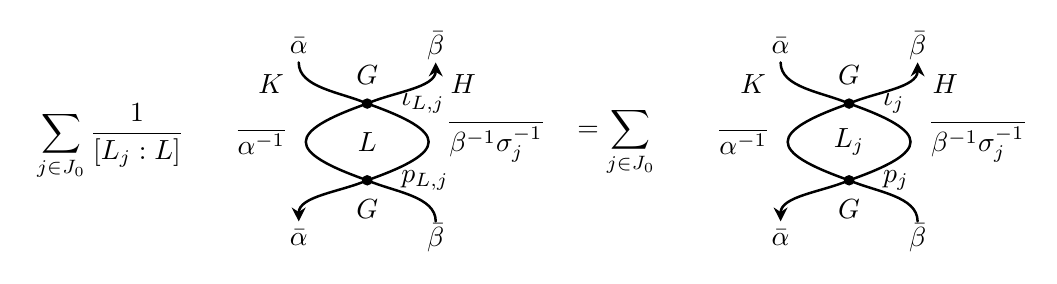
\begin{tikzpicture}[x=1cm,y=.87cm]
\node at (0,0) {$\displaystyle\sum_{j\in J_0}\frac{1}{[L_j:L]}$};
\begin{scope}[shift={(3.26,0)}]
\draw[arrowatend] (.87,-1.16)
   .. controls (.87,-.79) and (.34,-.73) .. (0,-.56)
   .. controls (-1.04,-.14) and (-1.04,.14) .. (0,.56)
   .. controls (.34,.73) and (.87,.79) .. (.87,1.16);
 \draw[arrowatend] (-.87,1.16)
   .. controls (-.87,.79) and (-.34,.73) .. (0,.56)
   .. controls (1.04,.14) and (1.04,-.14) .. (0,-.56)
   .. controls (-.34,-.73) and (-.87,-.79) .. (-.87,-1.16);
\fill (0,-0.56) circle (1.9pt);
\fill (0,0.56) circle (1.9pt);
\node[region] at (0,-0.98) {$G$};
\node[region] at (0,0.98) {$G$};
\node[region] at (0,0) {$L$};
\node[region] at (-1.22,.84) {$K$};
\node[region] at (1.22,.84) {$H$};
\node[strandlabel,anchor=east] at (-.99,0) {$\overline{\alpha^{-1}}$};
\node[strandlabel,anchor=west] at (.99,0) {$\overline{\beta^{-1}\sigma_j^{-1}}$};
\node[strandlabel,anchor=west] at (0.38,-0.56) {$p_{L,j}$};
\node[strandlabel,anchor=west] at (0.38,0.56) {$\iota_{L,j}$};
\node[strandlabel] at (-0.87,-1.4) {$\bar\alpha$};
\node[strandlabel] at (0.87,-1.4) {$\bar\beta$};
\node[strandlabel] at (-0.87,1.4) {$\bar\alpha$};
\node[strandlabel] at (0.87,1.4) {$\bar\beta$};
\end{scope}
\node at (6.42,0) {$=\displaystyle\sum_{j\in J_0}$};
\begin{scope}[shift={(9.38,0)}]
\draw[arrowatend] (.87,-1.16)
   .. controls (.87,-.79) and (.34,-.73) .. (0,-.56)
   .. controls (-1.04,-.14) and (-1.04,.14) .. (0,.56)
   .. controls (.34,.73) and (.87,.79) .. (.87,1.16);
 \draw[arrowatend] (-.87,1.16)
   .. controls (-.87,.79) and (-.34,.73) .. (0,.56)
   .. controls (1.04,.14) and (1.04,-.14) .. (0,-.56)
   .. controls (-.34,-.73) and (-.87,-.79) .. (-.87,-1.16);
\fill (0,-0.56) circle (1.9pt);
\fill (0,0.56) circle (1.9pt);
\node[region] at (0,-0.98) {$G$};
\node[region] at (0,0.98) {$G$};
\node[region] at (0,0) {$L_j$};
\node[region] at (-1.22,.84) {$K$};
\node[region] at (1.22,.84) {$H$};
\node[strandlabel,anchor=east] at (-.99,0) {$\overline{\alpha^{-1}}$};
\node[strandlabel,anchor=west] at (.99,0) {$\overline{\beta^{-1}\sigma_j^{-1}}$};
\node[strandlabel,anchor=west] at (0.38,-0.56) {$p_j$};
\node[strandlabel,anchor=west] at (0.38,0.56) {$\iota_j$};
\node[strandlabel] at (-0.87,-1.4) {$\bar\alpha$};
\node[strandlabel] at (0.87,-1.4) {$\bar\beta$};
\node[strandlabel] at (-0.87,1.4) {$\bar\alpha$};
\node[strandlabel] at (0.87,1.4) {$\bar\beta$};
\end{scope}
\end{tikzpicture}
\end{center}

In the reverse order the composite \(p_{L,j}\circ\iota_{L,j}\)
sums the fiber through each basis vector, as in
Proposition~\ref{prop:r2-mixed-composition}.

\begin{center}
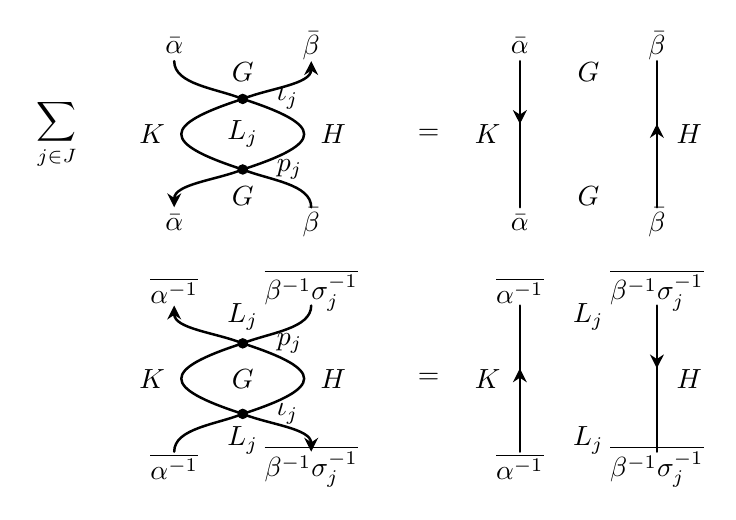
\begin{tikzpicture}[x=1cm,y=.80cm]
\node at (0,1.94) {$\displaystyle\sum_{j\in J}$};
\begin{scope}[shift={(2.36,1.94)}]
\draw[arrowatend] (.87,-1.16)
   .. controls (.87,-.79) and (.34,-.73) .. (0,-.56)
   .. controls (-1.04,-.14) and (-1.04,.14) .. (0,.56)
   .. controls (.34,.73) and (.87,.79) .. (.87,1.16);
 \draw[arrowatend] (-.87,1.16)
   .. controls (-.87,.79) and (-.34,.73) .. (0,.56)
   .. controls (1.04,.14) and (1.04,-.14) .. (0,-.56)
   .. controls (-.34,-.73) and (-.87,-.79) .. (-.87,-1.16);
\fill (0,-0.56) circle (1.9pt);
\fill (0,0.56) circle (1.9pt);
\node[region] at (0,-0.98) {$G$};
\node[region] at (0,0.98) {$G$};
\node[region] at (0,0) {$L_j$};
\node[region] at (-1.15,0) {$K$};
\node[region] at (1.15,0) {$H$};
\node[strandlabel,anchor=west] at (0.38,-0.56) {$p_j$};
\node[strandlabel,anchor=west] at (0.38,0.56) {$\iota_j$};
\node[strandlabel] at (-0.87,-1.4) {$\bar\alpha$};
\node[strandlabel] at (0.87,-1.4) {$\bar\beta$};
\node[strandlabel] at (-0.87,1.4) {$\bar\alpha$};
\node[strandlabel] at (0.87,1.4) {$\bar\beta$};
\end{scope}
\node at (4.72,1.94) {$=$};
\begin{scope}[shift={(6.75,1.94)}]
\draw[reverseoriented] (-.87,-1.16)--(-.87,1.16);
 \draw[oriented] (.87,-1.16)--(.87,1.16);
\node[region] at (0,-0.98) {$G$};
\node[region] at (0,0.98) {$G$};
\node[region] at (-1.28,0) {$K$};
\node[region] at (1.28,0) {$H$};
\node[strandlabel] at (-0.87,-1.4) {$\bar\alpha$};
\node[strandlabel] at (0.87,-1.4) {$\bar\beta$};
\node[strandlabel] at (-0.87,1.4) {$\bar\alpha$};
\node[strandlabel] at (0.87,1.4) {$\bar\beta$};
\end{scope}
\begin{scope}[shift={(2.36,-1.94)}]
\draw[arrowatstart] (.87,-1.16)
   .. controls (.87,-.79) and (.34,-.73) .. (0,-.56)
   .. controls (-1.04,-.14) and (-1.04,.14) .. (0,.56)
   .. controls (.34,.73) and (.87,.79) .. (.87,1.16);
 \draw[arrowatstart] (-.87,1.16)
   .. controls (-.87,.79) and (-.34,.73) .. (0,.56)
   .. controls (1.04,.14) and (1.04,-.14) .. (0,-.56)
   .. controls (-.34,-.73) and (-.87,-.79) .. (-.87,-1.16);
\fill (0,-0.56) circle (1.9pt);
\fill (0,0.56) circle (1.9pt);
\node[region] at (0,-0.98) {$L_j$};
\node[region] at (0,0.98) {$L_j$};
\node[region] at (0,0) {$G$};
\node[region] at (-1.15,0) {$K$};
\node[region] at (1.15,0) {$H$};
\node[strandlabel,anchor=west] at (0.38,-0.56) {$\iota_j$};
\node[strandlabel,anchor=west] at (0.38,0.56) {$p_j$};
\node[strandlabel] at (-0.87,-1.4) {$\overline{\alpha^{-1}}$};
\node[strandlabel] at (0.87,-1.4) {$\overline{\beta^{-1}\sigma_j^{-1}}$};
\node[strandlabel] at (-0.87,1.4) {$\overline{\alpha^{-1}}$};
\node[strandlabel] at (0.87,1.4) {$\overline{\beta^{-1}\sigma_j^{-1}}$};
\end{scope}
\node at (4.72,-1.94) {$=$};
\begin{scope}[shift={(6.75,-1.94)}]
\draw[oriented] (-.87,-1.16)--(-.87,1.16);
 \draw[reverseoriented] (.87,-1.16)--(.87,1.16);
\node[region] at (0,-0.98) {$L_j$};
\node[region] at (0,0.98) {$L_j$};
\node[region] at (-1.28,0) {$K$};
\node[region] at (1.28,0) {$H$};
\node[strandlabel] at (-0.87,-1.4) {$\overline{\alpha^{-1}}$};
\node[strandlabel] at (0.87,-1.4) {$\overline{\beta^{-1}\sigma_j^{-1}}$};
\node[strandlabel] at (-0.87,1.4) {$\overline{\alpha^{-1}}$};
\node[strandlabel] at (0.87,1.4) {$\overline{\beta^{-1}\sigma_j^{-1}}$};
\end{scope}
\end{tikzpicture}
\end{center}

When all double cosets are selected, the sum through the full
Mackey groups \(L_j\) is the identity on the boundary with middle
group \(G\). For a single full summand the reverse composite is
the identity on its balanced product.

\begin{center}
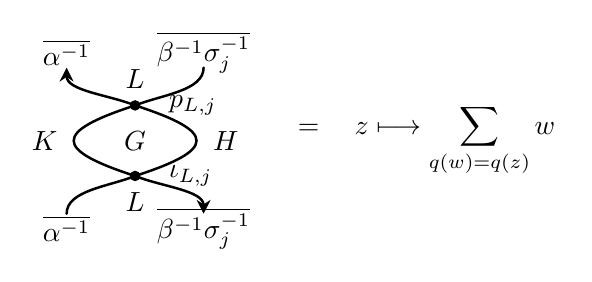
\begin{tikzpicture}[x=1cm,y=.80cm]
\begin{scope}[shift={(0,0)}]
\draw[arrowatstart] (.87,-1.16)
   .. controls (.87,-.79) and (.34,-.73) .. (0,-.56)
   .. controls (-1.04,-.14) and (-1.04,.14) .. (0,.56)
   .. controls (.34,.73) and (.87,.79) .. (.87,1.16);
 \draw[arrowatstart] (-.87,1.16)
   .. controls (-.87,.79) and (-.34,.73) .. (0,.56)
   .. controls (1.04,.14) and (1.04,-.14) .. (0,-.56)
   .. controls (-.34,-.73) and (-.87,-.79) .. (-.87,-1.16);
\fill (0,-0.56) circle (1.9pt);
\fill (0,0.56) circle (1.9pt);
\node[region] at (0,-0.98) {$L$};
\node[region] at (0,0.98) {$L$};
\node[region] at (0,0) {$G$};
\node[region] at (-1.15,0) {$K$};
\node[region] at (1.15,0) {$H$};
\node[strandlabel,anchor=west] at (0.38,-0.56) {$\iota_{L,j}$};
\node[strandlabel,anchor=west] at (0.38,0.56) {$p_{L,j}$};
\node[strandlabel] at (-0.87,-1.4) {$\overline{\alpha^{-1}}$};
\node[strandlabel] at (0.87,-1.4) {$\overline{\beta^{-1}\sigma_j^{-1}}$};
\node[strandlabel] at (-0.87,1.4) {$\overline{\alpha^{-1}}$};
\node[strandlabel] at (0.87,1.4) {$\overline{\beta^{-1}\sigma_j^{-1}}$};
\end{scope}
\node at (3.7,0) {$\displaystyle=\quad z\longmapsto\sum_{q(w)=q(z)}w$};
\end{tikzpicture}
\end{center}


\begin{example}[The common parabolic depends on the representatives]\label{ex:common-mackey-representatives}
Let \(G=S_3\times S_5\) on the blocks \(\{1,2,3\}\) and
\(\{4,5,6,7,8\}\), with \(K=H=\langle(12)\rangle\times S_5\)
and inclusion labels. The two double cosets have representatives
\(1,(13)(456)\). Their Mackey groups intersect in the second
factor, but the common-label condition gives
\(P=\langle(456)\rangle\times\langle(78)\rangle\).
The largest common parabolic is \(\langle(78)\rangle\).
Choosing \(1,(13)\) instead gives the full second factor as the
largest common parabolic, with indices \(2\) and \(1\).

\begin{center}
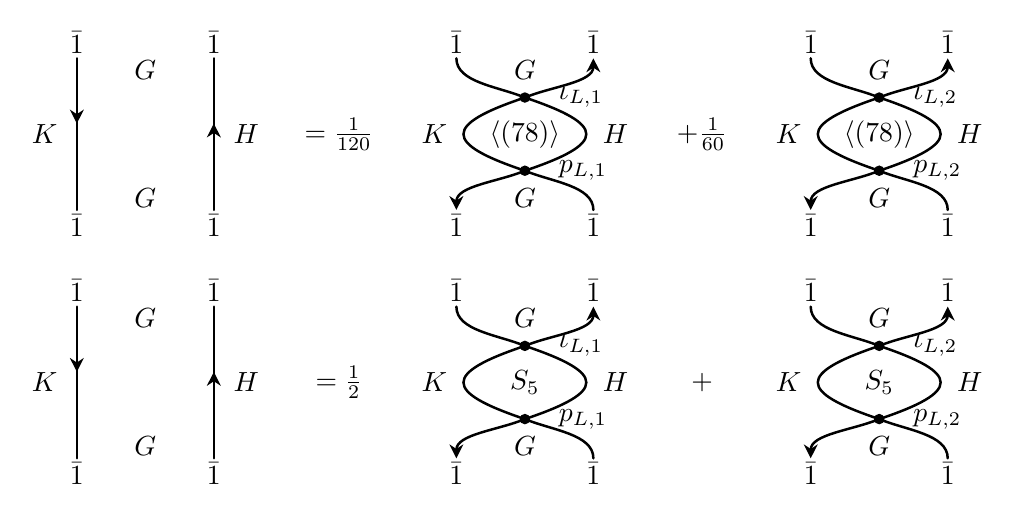
\begin{tikzpicture}[x=1cm,y=.83cm]
\begin{scope}[shift={(0,1.90)}]
\draw[reverseoriented] (-.87,-1.16)--(-.87,1.16);
 \draw[oriented] (.87,-1.16)--(.87,1.16);
\node[region] at (0,-0.98) {$G$};
\node[region] at (0,0.98) {$G$};
\node[region] at (-1.28,0) {$K$};
\node[region] at (1.28,0) {$H$};
\node[strandlabel] at (-0.87,-1.4) {$\bar1$};
\node[strandlabel] at (0.87,-1.4) {$\bar1$};
\node[strandlabel] at (-0.87,1.4) {$\bar1$};
\node[strandlabel] at (0.87,1.4) {$\bar1$};
\end{scope}
\node at (2.46,1.90) {$=\tfrac{1}{120}$};
\begin{scope}[shift={(4.82,1.90)}]
\draw[arrowatend] (.87,-1.16)
   .. controls (.87,-.79) and (.34,-.73) .. (0,-.56)
   .. controls (-1.04,-.14) and (-1.04,.14) .. (0,.56)
   .. controls (.34,.73) and (.87,.79) .. (.87,1.16);
 \draw[arrowatend] (-.87,1.16)
   .. controls (-.87,.79) and (-.34,.73) .. (0,.56)
   .. controls (1.04,.14) and (1.04,-.14) .. (0,-.56)
   .. controls (-.34,-.73) and (-.87,-.79) .. (-.87,-1.16);
\fill (0,-0.56) circle (1.9pt);
\fill (0,0.56) circle (1.9pt);
\node[region] at (0,-0.98) {$G$};
\node[region] at (0,0.98) {$G$};
\node[region] at (0,0) {$\langle(78)\rangle$};
\node[region] at (-1.15,0) {$K$};
\node[region] at (1.15,0) {$H$};
\node[strandlabel,anchor=west] at (0.38,-0.56) {$p_{L,1}$};
\node[strandlabel,anchor=west] at (0.38,0.56) {$\iota_{L,1}$};
\node[strandlabel] at (-0.87,-1.4) {$\bar1$};
\node[strandlabel] at (0.87,-1.4) {$\bar1$};
\node[strandlabel] at (-0.87,1.4) {$\bar1$};
\node[strandlabel] at (0.87,1.4) {$\bar1$};
\end{scope}
\node at (7.07,1.90) {$+\tfrac{1}{60}$};
\begin{scope}[shift={(9.32,1.90)}]
\draw[arrowatend] (.87,-1.16)
   .. controls (.87,-.79) and (.34,-.73) .. (0,-.56)
   .. controls (-1.04,-.14) and (-1.04,.14) .. (0,.56)
   .. controls (.34,.73) and (.87,.79) .. (.87,1.16);
 \draw[arrowatend] (-.87,1.16)
   .. controls (-.87,.79) and (-.34,.73) .. (0,.56)
   .. controls (1.04,.14) and (1.04,-.14) .. (0,-.56)
   .. controls (-.34,-.73) and (-.87,-.79) .. (-.87,-1.16);
\fill (0,-0.56) circle (1.9pt);
\fill (0,0.56) circle (1.9pt);
\node[region] at (0,-0.98) {$G$};
\node[region] at (0,0.98) {$G$};
\node[region] at (0,0) {$\langle(78)\rangle$};
\node[region] at (-1.15,0) {$K$};
\node[region] at (1.15,0) {$H$};
\node[strandlabel,anchor=west] at (0.38,-0.56) {$p_{L,2}$};
\node[strandlabel,anchor=west] at (0.38,0.56) {$\iota_{L,2}$};
\node[strandlabel] at (-0.87,-1.4) {$\bar1$};
\node[strandlabel] at (0.87,-1.4) {$\bar1$};
\node[strandlabel] at (-0.87,1.4) {$\bar1$};
\node[strandlabel] at (0.87,1.4) {$\bar1$};
\end{scope}
\begin{scope}[shift={(0,-1.90)}]
\draw[reverseoriented] (-.87,-1.16)--(-.87,1.16);
 \draw[oriented] (.87,-1.16)--(.87,1.16);
\node[region] at (0,-0.98) {$G$};
\node[region] at (0,0.98) {$G$};
\node[region] at (-1.28,0) {$K$};
\node[region] at (1.28,0) {$H$};
\node[strandlabel] at (-0.87,-1.4) {$\bar1$};
\node[strandlabel] at (0.87,-1.4) {$\bar1$};
\node[strandlabel] at (-0.87,1.4) {$\bar1$};
\node[strandlabel] at (0.87,1.4) {$\bar1$};
\end{scope}
\node at (2.46,-1.90) {$=\tfrac12$};
\begin{scope}[shift={(4.82,-1.90)}]
\draw[arrowatend] (.87,-1.16)
   .. controls (.87,-.79) and (.34,-.73) .. (0,-.56)
   .. controls (-1.04,-.14) and (-1.04,.14) .. (0,.56)
   .. controls (.34,.73) and (.87,.79) .. (.87,1.16);
 \draw[arrowatend] (-.87,1.16)
   .. controls (-.87,.79) and (-.34,.73) .. (0,.56)
   .. controls (1.04,.14) and (1.04,-.14) .. (0,-.56)
   .. controls (-.34,-.73) and (-.87,-.79) .. (-.87,-1.16);
\fill (0,-0.56) circle (1.9pt);
\fill (0,0.56) circle (1.9pt);
\node[region] at (0,-0.98) {$G$};
\node[region] at (0,0.98) {$G$};
\node[region] at (0,0) {$S_5$};
\node[region] at (-1.15,0) {$K$};
\node[region] at (1.15,0) {$H$};
\node[strandlabel,anchor=west] at (0.38,-0.56) {$p_{L,1}$};
\node[strandlabel,anchor=west] at (0.38,0.56) {$\iota_{L,1}$};
\node[strandlabel] at (-0.87,-1.4) {$\bar1$};
\node[strandlabel] at (0.87,-1.4) {$\bar1$};
\node[strandlabel] at (-0.87,1.4) {$\bar1$};
\node[strandlabel] at (0.87,1.4) {$\bar1$};
\end{scope}
\node at (7.07,-1.90) {$+$};
\begin{scope}[shift={(9.32,-1.90)}]
\draw[arrowatend] (.87,-1.16)
   .. controls (.87,-.79) and (.34,-.73) .. (0,-.56)
   .. controls (-1.04,-.14) and (-1.04,.14) .. (0,.56)
   .. controls (.34,.73) and (.87,.79) .. (.87,1.16);
 \draw[arrowatend] (-.87,1.16)
   .. controls (-.87,.79) and (-.34,.73) .. (0,.56)
   .. controls (1.04,.14) and (1.04,-.14) .. (0,-.56)
   .. controls (-.34,-.73) and (-.87,-.79) .. (-.87,-1.16);
\fill (0,-0.56) circle (1.9pt);
\fill (0,0.56) circle (1.9pt);
\node[region] at (0,-0.98) {$G$};
\node[region] at (0,0.98) {$G$};
\node[region] at (0,0) {$S_5$};
\node[region] at (-1.15,0) {$K$};
\node[region] at (1.15,0) {$H$};
\node[strandlabel,anchor=west] at (0.38,-0.56) {$p_{L,2}$};
\node[strandlabel,anchor=west] at (0.38,0.56) {$\iota_{L,2}$};
\node[strandlabel] at (-0.87,-1.4) {$\bar1$};
\node[strandlabel] at (0.87,-1.4) {$\bar1$};
\node[strandlabel] at (-0.87,1.4) {$\bar1$};
\node[strandlabel] at (0.87,1.4) {$\bar1$};
\end{scope}
\end{tikzpicture}
\end{center}
\end{example}


\begin{proposition}[Shared region for parallel crossings]\label{prop:parabolic-common-parallel-two}
Take a finite family of the parallel two-crossing diagrams of
Theorem~\ref{thm:r2-parallel}, with the same outside groups \(G,K\)
and prescribed middle composite conjugators \(v_i\). With inclusion
as the middle embedding into \(G\), the least common middle group is
\[
 P=\left\langle\bigcup_i\cg{v_i}{K}\right\rangle.
\]
Each diagram keeps its dots and its evaluated map. In the diagram
\(B_i\) denotes the original middle group.
\end{proposition}

\begin{proof}
The middle group must contain every \(\cg{v_i}{K}\). Their join is
parabolic. Factor each embedding of \(K\) through this join by
conjugation by \(v_i\), followed by inclusion into \(G\). The
composite embeddings and the conditions on the dots are unchanged.
Theorem~\ref{thm:r2-parallel} therefore gives the same evaluated map,
for both induction and restriction.
\end{proof}

\begin{center}
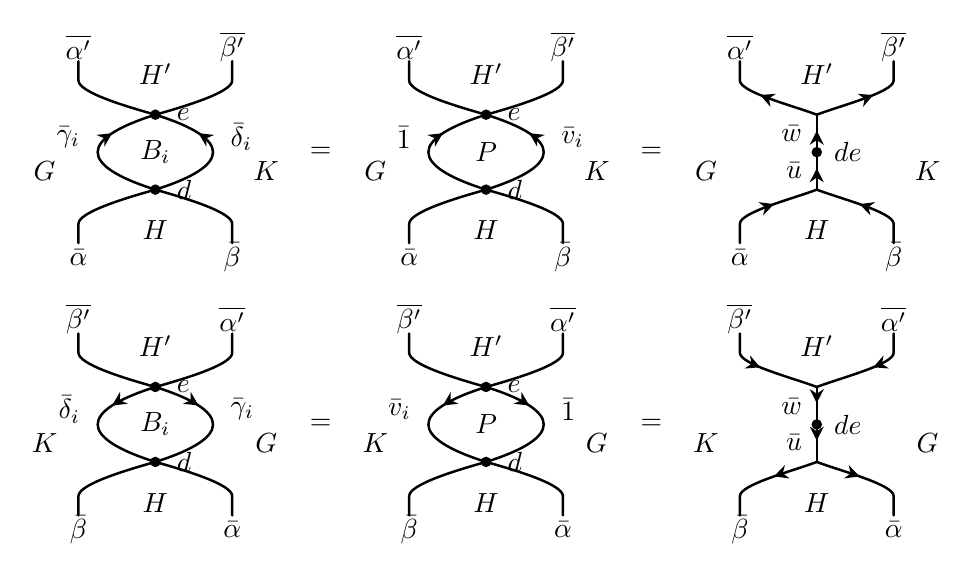
\begin{tikzpicture}[x=1.05cm,y=.70cm]
\begin{scope}[shift={(0,2.47)}]
\foreach \slot in {-1,1} {
      \begin{scope}[xscale=\slot]
       \draw[oriented] (-.93,-1.65)--(-.93,-1.30)
       .. controls (-.93,-1.09) and (-.38,-.84) .. (0,-.68)
       .. controls (.93,-.24) and (.93,.24) .. (0,.68)
       .. controls (-.38,.84) and (-.93,1.09) .. (-.93,1.30)
       --(-.93,1.65);
      \end{scope}
    }
\fill (0,-0.68) circle (1.9pt);
\fill (0,0.68) circle (1.9pt);
\node[strandlabel,anchor=west] at (0.21,-0.68) {$d$};
\node[strandlabel,anchor=west] at (0.21,0.68) {$e$};
\node[region] at (0,0) {$B_i$};
\node[strandlabel,anchor=east] at (-0.86,0.27) {$\bar\gamma_i$};
\node[strandlabel,anchor=west] at (0.86,0.27) {$\bar\delta_i$};
\node[region] at (-1.34,-0.34) {$G$};
\node[region] at (1.34,-0.34) {$K$};
\node[region] at (0,-1.42) {$H$};
\node[region] at (0,1.42) {$H'$};
\node[strandlabel] at (-0.93,-1.91) {$\bar\alpha$};
\node[strandlabel] at (0.93,-1.91) {$\bar\beta$};
\node[strandlabel] at (-0.93,1.91) {$\overline{\alpha'}$};
\node[strandlabel] at (0.93,1.91) {$\overline{\beta'}$};
\end{scope}
\node at (2,2.47) {$=$};
\begin{scope}[shift={(4,2.47)}]
\foreach \slot in {-1,1} {
      \begin{scope}[xscale=\slot]
       \draw[oriented] (-.93,-1.65)--(-.93,-1.30)
       .. controls (-.93,-1.09) and (-.38,-.84) .. (0,-.68)
       .. controls (.93,-.24) and (.93,.24) .. (0,.68)
       .. controls (-.38,.84) and (-.93,1.09) .. (-.93,1.30)
       --(-.93,1.65);
      \end{scope}
    }
\fill (0,-0.68) circle (1.9pt);
\fill (0,0.68) circle (1.9pt);
\node[strandlabel,anchor=west] at (0.21,-0.68) {$d$};
\node[strandlabel,anchor=west] at (0.21,0.68) {$e$};
\node[region] at (0,0) {$P$};
\node[strandlabel,anchor=east] at (-0.86,0.27) {$\bar 1$};
\node[strandlabel,anchor=west] at (0.86,0.27) {$\bar v_i$};
\node[region] at (-1.34,-0.34) {$G$};
\node[region] at (1.34,-0.34) {$K$};
\node[region] at (0,-1.42) {$H$};
\node[region] at (0,1.42) {$H'$};
\node[strandlabel] at (-0.93,-1.91) {$\bar\alpha$};
\node[strandlabel] at (0.93,-1.91) {$\bar\beta$};
\node[strandlabel] at (-0.93,1.91) {$\overline{\alpha'}$};
\node[strandlabel] at (0.93,1.91) {$\overline{\beta'}$};
\end{scope}
\node at (6,2.47) {$=$};
\begin{scope}[shift={(8,2.47)}]
\draw[oriented] (-.93,-1.65)--(-.93,-1.30)
       .. controls (-.93,-1.09) and (-.30,-.85) .. (0,-.68);
    \draw[oriented] (.93,-1.65)--(.93,-1.30)
       .. controls (.93,-1.09) and (.30,-.85) .. (0,-.68);
    \draw[oriented] (0,-.68)--(0,0);
    \draw[oriented] (0,0)--(0,.68);
    \draw[oriented] (0,.68)
       .. controls (-.30,.85) and (-.93,1.09) .. (-.93,1.30)--(-.93,1.65);
    \draw[oriented] (0,.68)
       .. controls (.30,.85) and (.93,1.09) .. (.93,1.30)--(.93,1.65);
\fill (0,0) circle (1.9pt);
\node[strandlabel,anchor=west] at (0.16,0) {$de$};
\node[strandlabel,anchor=east] at (-0.13,-0.33) {$\bar u$};
\node[strandlabel,anchor=east] at (-0.13,0.33) {$\bar w$};
\node[region] at (-1.34,-0.34) {$G$};
\node[region] at (1.34,-0.34) {$K$};
\node[region] at (0,-1.42) {$H$};
\node[region] at (0,1.42) {$H'$};
\node[strandlabel] at (-0.93,-1.91) {$\bar\alpha$};
\node[strandlabel] at (0.93,-1.91) {$\bar\beta$};
\node[strandlabel] at (-0.93,1.91) {$\overline{\alpha'}$};
\node[strandlabel] at (0.93,1.91) {$\overline{\beta'}$};
\end{scope}
\begin{scope}[shift={(0,-2.47)}]
\foreach \slot in {-1,1} {
      \begin{scope}[xscale=\slot]
       \draw[reverseoriented] (-.93,-1.65)--(-.93,-1.30)
       .. controls (-.93,-1.09) and (-.38,-.84) .. (0,-.68)
       .. controls (.93,-.24) and (.93,.24) .. (0,.68)
       .. controls (-.38,.84) and (-.93,1.09) .. (-.93,1.30)
       --(-.93,1.65);
      \end{scope}
    }
\fill (0,-0.68) circle (1.9pt);
\fill (0,0.68) circle (1.9pt);
\node[strandlabel,anchor=west] at (0.21,-0.68) {$d$};
\node[strandlabel,anchor=west] at (0.21,0.68) {$e$};
\node[region] at (0,0) {$B_i$};
\node[strandlabel,anchor=west] at (0.86,0.27) {$\bar\gamma_i$};
\node[strandlabel,anchor=east] at (-0.86,0.27) {$\bar\delta_i$};
\node[region] at (-1.34,-0.34) {$K$};
\node[region] at (1.34,-0.34) {$G$};
\node[region] at (0,-1.42) {$H$};
\node[region] at (0,1.42) {$H'$};
\node[strandlabel] at (0.93,-1.91) {$\bar\alpha$};
\node[strandlabel] at (-0.93,-1.91) {$\bar\beta$};
\node[strandlabel] at (0.93,1.91) {$\overline{\alpha'}$};
\node[strandlabel] at (-0.93,1.91) {$\overline{\beta'}$};
\end{scope}
\node at (2,-2.47) {$=$};
\begin{scope}[shift={(4,-2.47)}]
\foreach \slot in {-1,1} {
      \begin{scope}[xscale=\slot]
       \draw[reverseoriented] (-.93,-1.65)--(-.93,-1.30)
       .. controls (-.93,-1.09) and (-.38,-.84) .. (0,-.68)
       .. controls (.93,-.24) and (.93,.24) .. (0,.68)
       .. controls (-.38,.84) and (-.93,1.09) .. (-.93,1.30)
       --(-.93,1.65);
      \end{scope}
    }
\fill (0,-0.68) circle (1.9pt);
\fill (0,0.68) circle (1.9pt);
\node[strandlabel,anchor=west] at (0.21,-0.68) {$d$};
\node[strandlabel,anchor=west] at (0.21,0.68) {$e$};
\node[region] at (0,0) {$P$};
\node[strandlabel,anchor=west] at (0.86,0.27) {$\bar 1$};
\node[strandlabel,anchor=east] at (-0.86,0.27) {$\bar v_i$};
\node[region] at (-1.34,-0.34) {$K$};
\node[region] at (1.34,-0.34) {$G$};
\node[region] at (0,-1.42) {$H$};
\node[region] at (0,1.42) {$H'$};
\node[strandlabel] at (0.93,-1.91) {$\bar\alpha$};
\node[strandlabel] at (-0.93,-1.91) {$\bar\beta$};
\node[strandlabel] at (0.93,1.91) {$\overline{\alpha'}$};
\node[strandlabel] at (-0.93,1.91) {$\overline{\beta'}$};
\end{scope}
\node at (6,-2.47) {$=$};
\begin{scope}[shift={(8,-2.47)}]
\draw[reverseoriented] (-.93,-1.65)--(-.93,-1.30)
       .. controls (-.93,-1.09) and (-.30,-.85) .. (0,-.68);
    \draw[reverseoriented] (.93,-1.65)--(.93,-1.30)
       .. controls (.93,-1.09) and (.30,-.85) .. (0,-.68);
    \draw[reverseoriented] (0,-.68)--(0,0);
    \draw[reverseoriented] (0,0)--(0,.68);
    \draw[reverseoriented] (0,.68)
       .. controls (-.30,.85) and (-.93,1.09) .. (-.93,1.30)--(-.93,1.65);
    \draw[reverseoriented] (0,.68)
       .. controls (.30,.85) and (.93,1.09) .. (.93,1.30)--(.93,1.65);
\fill (0,0) circle (1.9pt);
\node[strandlabel,anchor=west] at (0.16,0) {$de$};
\node[strandlabel,anchor=east] at (-0.13,-0.33) {$\bar u$};
\node[strandlabel,anchor=east] at (-0.13,0.33) {$\bar w$};
\node[region] at (-1.34,-0.34) {$K$};
\node[region] at (1.34,-0.34) {$G$};
\node[region] at (0,-1.42) {$H$};
\node[region] at (0,1.42) {$H'$};
\node[strandlabel] at (0.93,-1.91) {$\bar\alpha$};
\node[strandlabel] at (-0.93,-1.91) {$\bar\beta$};
\node[strandlabel] at (0.93,1.91) {$\overline{\alpha'}$};
\node[strandlabel] at (-0.93,1.91) {$\overline{\beta'}$};
\end{scope}
\end{tikzpicture}
\end{center}

\subsection{Reidemeister III}

For three induction strands, the constructions of
Lemma~\ref{lem:reidemeister-three} use \(B'=F\) and \(B=G\).
Both are boundary groups, so the inverse bijections on evaluation
classes restrict to this category. In Cases~1--4 the usual
single-diagram replacements can use \(B'=A\) and \(B=E\).
The following choices give sharper bounds for group-element dots.

\begin{proposition}[Extremal regions for three induction strands]\label{prop:parabolic-three-induction}
Use the boundary labels of Section~\ref{sec:reidemeister-three}.
Write \(a=\boxed{GA}\), \(d=\boxed{AD}\), \(c=\boxed{GC}\), and
\(e=\boxed{CE}\). For an admissible group-element multiplier
\(p\in G\) and diagrams with group-element dots, the least
transported left region and the greatest
transported right region are, respectively,
\[
 B_{\min}=\left\langle\cg{ad}{D},\cg{pce}{E}\right\rangle,
 \qquad
 B'_{\max}=\cg{a}{A}\cap\cg{pc}{C}.
\]
With these regions, both diagrams evaluate to \(x\mapsto xp\).
\end{proposition}

\begin{proof}
For left dots \(x_1,x_2,x_3\), transport the region \(B\) into \(G\)
by \(x_1\boxed{GB}\). The two outside vertex conditions put
\(\cg{ad}{D}\) and \(\cg{x_1x_3ce}{E}\) in the transported region.
Conjugating the latter by
\(x_1(\boxed{GB})_*(x_2)x_1^{-1}\), an element of the transported
region, puts \(\cg{pce}{E}\) there as well, by the multiplier
formula in Lemma~\ref{lem:reidemeister-three}. Thus the region
contains the displayed join. To attain it, take that join as
\(B\), use \(\boxed{GB}=1\), \(\boxed{BD}=ad\), \(\boxed{BE}=pce\),
and use dots \((1,1,p)\). The middle embeddings of \(F\) agree
because \(p\) intertwines the two boundary embeddings.

For right dots \(y_1,y_2,y_3\), transport \(B'\) by
\(a y_1\boxed{AB'}\). Its image lies in \(\cg{a}{A}\). By the
middle vertex it also lies in \(\cg{pc}{C}\), since
\(p=(\boxed{GA})_*(y_1)y_2(\boxed{GC})_*(y_3)\) and the last factor
belongs to \(\cg{c}{C}\). The lower vertex puts \(\cg{u}{F}\) in
the transported region, where \(u\) is the bottom composite.
To attain the intersection, take it as \(B'\) and use
\(\boxed{AB'}=a^{-1}\), \(\boxed{CB'}=c^{-1}p^{-1}\),
\(\boxed{B'F}=u\), and dots \((1,p,1)\). The bottom outside
composite is the prescribed embedding of \(F\) into \(A\).
The top outside composite is the prescribed embedding into \(C\)
because \(p\) intertwines the boundary embeddings. The middle
dot is \(p\). Join and intersection closure keep both choices
parabolic.
\end{proof}

\begin{center}
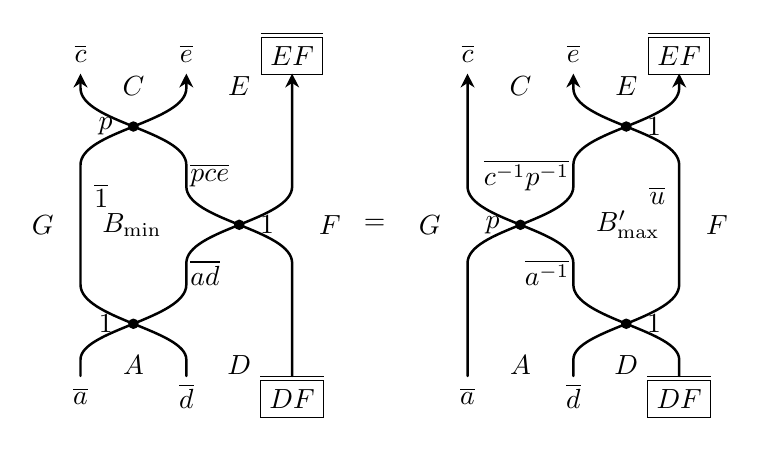
\begin{tikzpicture}[x=.96cm,y=.80cm]
\mixedThreeWires{arrowatend}{arrowatend}{arrowatend}
\node[region] at (-0.5,2.4) {$G$};
\node[region] at (0.7,0.18) {$A$};
\node[region] at (2.1,0.18) {$D$};
\node[region] at (0.7,4.6) {$C$};
\node[region] at (2.1,4.6) {$E$};
\node[region] at (3.3,2.4) {$F$};
\node[strandlabel] at (0,-0.32) {$\overline{a}$};
\node[strandlabel] at (1.4,-0.32) {$\overline{d}$};
\node[strandlabel] at (2.8,-0.32) {$\overline{\boxed{DF}}$};
\node[strandlabel] at (0,5.12) {$\overline{c}$};
\node[strandlabel] at (1.4,5.12) {$\overline{e}$};
\node[strandlabel] at (2.8,5.12) {$\overline{\boxed{EF}}$};
\node[region] at (0.68,2.4) {$B_{\min}$};
\fill (0.7,0.82875) circle (1.9pt);
\node[strandlabel,anchor=east] at (0.48,0.82875) {$1$};
\fill (2.1,2.4) circle (1.9pt);
\node[strandlabel,anchor=west] at (2.32,2.4) {$1$};
\fill (0.7,3.96) circle (1.9pt);
\node[strandlabel,anchor=east] at (0.48,3.96) {$p$};
\node[strandlabel,anchor=west] at (0.13,2.86) {$\overline{1}$};
\node[strandlabel,anchor=west] at (1.4,1.64) {$\overline{ad}$};
\node[strandlabel,anchor=west] at (1.4,3.18) {$\overline{pce}$};
\node at (3.89,2.4) {$=$};
\begin{scope}[shift={(5.12,0)}]
\begin{scope}[shift={(2.8,0)},xscale=-1]
\mixedThreeWires{arrowatend}{arrowatend}{arrowatend}
\end{scope}
\node[region] at (-0.5,2.4) {$G$};
\node[region] at (0.7,0.18) {$A$};
\node[region] at (2.1,0.18) {$D$};
\node[region] at (0.7,4.6) {$C$};
\node[region] at (2.1,4.6) {$E$};
\node[region] at (3.3,2.4) {$F$};
\node[strandlabel] at (0,-0.32) {$\overline{a}$};
\node[strandlabel] at (1.4,-0.32) {$\overline{d}$};
\node[strandlabel] at (2.8,-0.32) {$\overline{\boxed{DF}}$};
\node[strandlabel] at (0,5.12) {$\overline{c}$};
\node[strandlabel] at (1.4,5.12) {$\overline{e}$};
\node[strandlabel] at (2.8,5.12) {$\overline{\boxed{EF}}$};
\node[region] at (2.12,2.4) {$B'_{\max}$};
\fill (2.1,0.82875) circle (1.9pt);
\node[strandlabel,anchor=west] at (2.32,0.82875) {$1$};
\fill (0.7,2.4) circle (1.9pt);
\node[strandlabel,anchor=east] at (0.48,2.4) {$p$};
\fill (2.1,3.96) circle (1.9pt);
\node[strandlabel,anchor=west] at (2.32,3.96) {$1$};
\node[strandlabel,anchor=east] at (2.67,2.86) {$\overline{u}$};
\node[strandlabel,anchor=east] at (1.4,1.64) {$\overline{a^{-1}}$};
\node[strandlabel,anchor=east] at (1.4,3.18) {$\overline{c^{-1}p^{-1}}$};
\end{scope}
\end{tikzpicture}
\end{center}


\begin{example}[Extremal internal groups for three inductions]\label{ex:three-induction-extrema}
For inclusion labels with \(G=S_4\), \(A=D=\langle(12)\rangle\),
\(C=E=\langle(23)\rangle\), \(F=1\) and \(p=1\), the left minimum
is \(\operatorname{Sym}(\{1,2,3\})\) and the right maximum is \(1\).
\end{example}

Linear dots give sums of the single-crossing element identities.

\begin{proposition}[Extremal regions in Cases 1--4]\label{prop:parabolic-three-outside}
Use the embeddings \(a,b,c,d,e,f\) of Cases~1--4 and fix an
admissible group-element crossing element \(p\in A\).
For Cases~1 and~3 the least transported right region is
\[
 P_p=\left\langle (ad)(C),\,p(bc)(F)p^{-1}\right\rangle.
\]
For Cases~2 and~4 the greatest transported left region is
\(B_{\max}=a(G)\cap p b(D)p^{-1}\). More precisely, every parabolic \(B\)
in the interval
\[
 (ade)(E)\le B\le a(G)\cap p b(D)p^{-1}
\]
is a possible transported left region. With the largest choice
in Case~2 the first projection has one preimage on its image.
\end{proposition}

\begin{proof}
In the notation of Theorem~\ref{thm:three-projections}, the right
region transported by \(m u\) contains \((ad)(C)\) by the middle
vertex. The lower vertex and \(p=m u(n)\ell^{-1}\) put
\(p(bc)(F)p^{-1}=m u(n w(F)n^{-1})m^{-1}\) in the same region.
The proof of that theorem attains the join using \(B'=P_p\),
the inclusion \(u\), \(v=ad\), \(w=\operatorname{Ad}_p\circ bc\),
and \((\ell,m,n)=(p^{-1},1,1)\). The reversed arrows in Case~3
give the same group and the multiplication map.

In the left diagram, transport the image \(a r(B)\) by \(a(z^{-1})\)
using the notation of Lemma~\ref{lem:three-projections}. It
contains \((ade)(E)\) by the upper vertex, is contained in \(a(G)\),
and is contained in \(p b(D)p^{-1}\) by the lower vertex and
\(p=a(z^{-1})x b(y)\). Conversely, for any \(B\) in the interval,
take \(r=a^{-1}|_B\),
\(s=b^{-1}\circ\operatorname{Ad}_{p^{-1}}|_B\), \(t=ade\),
and use \(x=p,\ y=z=1\). Here \(st=cf\) is the admissibility
condition on \(p\). In Case~2, transporting the two stabilizer
indices to \(A\) gives
\[
 [a(G)\cap p b(D)p^{-1}:B],\qquad
 [B\cap p(bc)(F)p^{-1}:(ade)(E)].
\]
Both indices are finite because the ambient groups are finite.
The first is \(1\) at the maximum. Reversing the arrows gives
the corresponding choice in Case~4.
\end{proof}

The projection diagrams below map \(\C[A]\) to the complex span of
\(G\times_E F\). Both send \(z\) to the sum of the preimages of \(z\)
under \(Q_p([g,h])=a(g)p(bc)(h)\). The mixed crossing labelled \(p\)
on the left uses trace dot \(p^{-1}\). On the right, the lower
crossing is between parallel strands and carries dot \(p^{-1}\).

\begin{center}
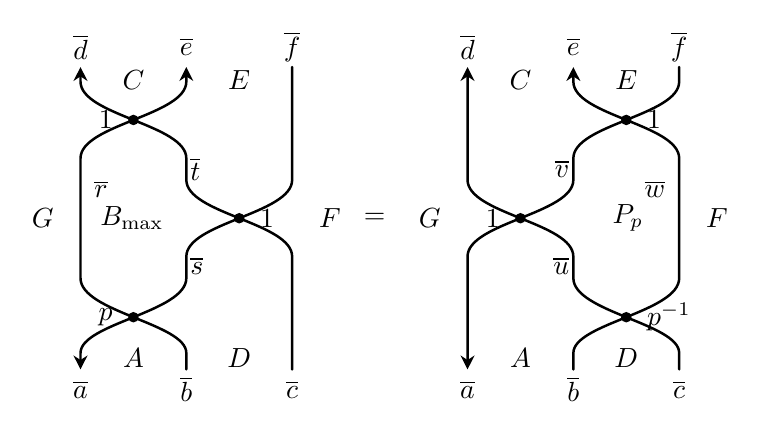
\begin{tikzpicture}[x=.96cm,y=.80cm]
\mixedThreeWires{arrowatstart}{arrowatend}{arrowatend}
\node[region] at (-0.5,2.4) {$G$};
\node[region] at (0.7,0.18) {$A$};
\node[region] at (2.1,0.18) {$D$};
\node[region] at (0.7,4.6) {$C$};
\node[region] at (2.1,4.6) {$E$};
\node[region] at (3.3,2.4) {$F$};
\node[strandlabel] at (0,-0.32) {$\overline{a}$};
\node[strandlabel] at (1.4,-0.32) {$\overline{b}$};
\node[strandlabel] at (2.8,-0.32) {$\overline{c}$};
\node[strandlabel] at (0,5.12) {$\overline{d}$};
\node[strandlabel] at (1.4,5.12) {$\overline{e}$};
\node[strandlabel] at (2.8,5.12) {$\overline{f}$};
\node[region] at (0.68,2.4) {$B_{\max}$};
\fill (0.7,0.82875) circle (1.9pt);
\node[strandlabel,anchor=east] at (0.48,0.82875) {$p$};
\fill (2.1,2.4) circle (1.9pt);
\node[strandlabel,anchor=west] at (2.32,2.4) {$1$};
\fill (0.7,3.96) circle (1.9pt);
\node[strandlabel,anchor=east] at (0.48,3.96) {$1$};
\node[strandlabel,anchor=west] at (0.13,2.86) {$\overline{r}$};
\node[strandlabel,anchor=west] at (1.4,1.64) {$\overline{s}$};
\node[strandlabel,anchor=west] at (1.4,3.18) {$\overline{t}$};
\node at (3.89,2.4) {$=$};
\begin{scope}[shift={(5.12,0)}]
\begin{scope}[shift={(2.8,0)},xscale=-1]
\mixedThreeWires{arrowatend}{arrowatend}{arrowatstart}
\end{scope}
\node[region] at (-0.5,2.4) {$G$};
\node[region] at (0.7,0.18) {$A$};
\node[region] at (2.1,0.18) {$D$};
\node[region] at (0.7,4.6) {$C$};
\node[region] at (2.1,4.6) {$E$};
\node[region] at (3.3,2.4) {$F$};
\node[strandlabel] at (0,-0.32) {$\overline{a}$};
\node[strandlabel] at (1.4,-0.32) {$\overline{b}$};
\node[strandlabel] at (2.8,-0.32) {$\overline{c}$};
\node[strandlabel] at (0,5.12) {$\overline{d}$};
\node[strandlabel] at (1.4,5.12) {$\overline{e}$};
\node[strandlabel] at (2.8,5.12) {$\overline{f}$};
\node[region] at (2.12,2.4) {$P_p$};
\fill (2.1,0.82875) circle (1.9pt);
\node[strandlabel,anchor=west] at (2.32,0.82875) {$p^{-1}$};
\fill (0.7,2.4) circle (1.9pt);
\node[strandlabel,anchor=east] at (0.48,2.4) {$1$};
\fill (2.1,3.96) circle (1.9pt);
\node[strandlabel,anchor=west] at (2.32,3.96) {$1$};
\node[strandlabel,anchor=east] at (2.67,2.86) {$\overline{w}$};
\node[strandlabel,anchor=east] at (1.4,1.64) {$\overline{u}$};
\node[strandlabel,anchor=east] at (1.4,3.18) {$\overline{v}$};
\end{scope}
\end{tikzpicture}
\end{center}

The multiplication diagrams below have the opposite source and
target. Each sends \([g,h]\) to \(a(g)p(bc)(h)\).

\begin{center}
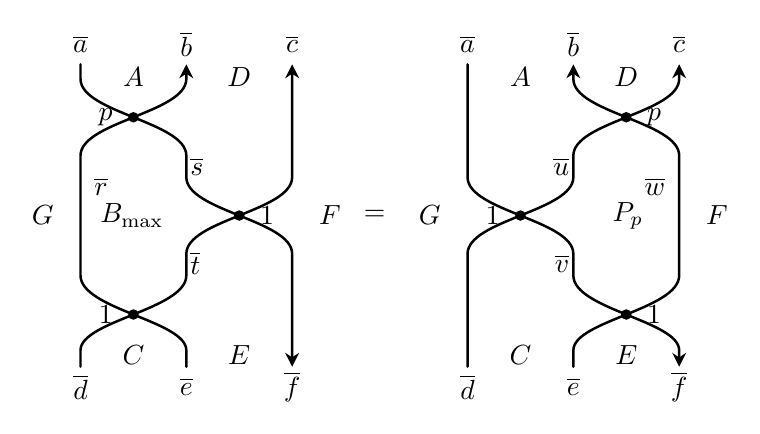
\begin{tikzpicture}[x=.96cm,y=.80cm]
\mixedThreeWires{arrowatend}{arrowatend}{arrowatstart}
\node[region] at (-0.5,2.4) {$G$};
\node[region] at (0.7,0.18) {$C$};
\node[region] at (2.1,0.18) {$E$};
\node[region] at (0.7,4.6) {$A$};
\node[region] at (2.1,4.6) {$D$};
\node[region] at (3.3,2.4) {$F$};
\node[strandlabel] at (0,-0.32) {$\overline{d}$};
\node[strandlabel] at (1.4,-0.32) {$\overline{e}$};
\node[strandlabel] at (2.8,-0.32) {$\overline{f}$};
\node[strandlabel] at (0,5.12) {$\overline{a}$};
\node[strandlabel] at (1.4,5.12) {$\overline{b}$};
\node[strandlabel] at (2.8,5.12) {$\overline{c}$};
\node[region] at (0.68,2.4) {$B_{\max}$};
\fill (0.7,0.82875) circle (1.9pt);
\node[strandlabel,anchor=east] at (0.48,0.82875) {$1$};
\fill (2.1,2.4) circle (1.9pt);
\node[strandlabel,anchor=west] at (2.32,2.4) {$1$};
\fill (0.7,3.96) circle (1.9pt);
\node[strandlabel,anchor=east] at (0.48,3.96) {$p$};
\node[strandlabel,anchor=west] at (0.13,2.86) {$\overline{r}$};
\node[strandlabel,anchor=west] at (1.4,1.64) {$\overline{t}$};
\node[strandlabel,anchor=west] at (1.4,3.18) {$\overline{s}$};
\node at (3.89,2.4) {$=$};
\begin{scope}[shift={(5.12,0)}]
\begin{scope}[shift={(2.8,0)},xscale=-1]
\mixedThreeWires{arrowatstart}{arrowatend}{arrowatend}
\end{scope}
\node[region] at (-0.5,2.4) {$G$};
\node[region] at (0.7,0.18) {$C$};
\node[region] at (2.1,0.18) {$E$};
\node[region] at (0.7,4.6) {$A$};
\node[region] at (2.1,4.6) {$D$};
\node[region] at (3.3,2.4) {$F$};
\node[strandlabel] at (0,-0.32) {$\overline{d}$};
\node[strandlabel] at (1.4,-0.32) {$\overline{e}$};
\node[strandlabel] at (2.8,-0.32) {$\overline{f}$};
\node[strandlabel] at (0,5.12) {$\overline{a}$};
\node[strandlabel] at (1.4,5.12) {$\overline{b}$};
\node[strandlabel] at (2.8,5.12) {$\overline{c}$};
\node[region] at (2.12,2.4) {$P_p$};
\fill (2.1,0.82875) circle (1.9pt);
\node[strandlabel,anchor=west] at (2.32,0.82875) {$1$};
\fill (0.7,2.4) circle (1.9pt);
\node[strandlabel,anchor=east] at (0.48,2.4) {$1$};
\fill (2.1,3.96) circle (1.9pt);
\node[strandlabel,anchor=west] at (2.32,3.96) {$p$};
\node[strandlabel,anchor=east] at (2.67,2.86) {$\overline{w}$};
\node[strandlabel,anchor=east] at (1.4,1.64) {$\overline{v}$};
\node[strandlabel,anchor=east] at (1.4,3.18) {$\overline{u}$};
\end{scope}
\end{tikzpicture}
\end{center}


\begin{example}[A smaller internal group reduces a projection fiber]\label{ex:case-one-parabolic-index}
In Case~1 take \(A=S_4\), \(G=\operatorname{Sym}(\{1,2,4\})\),
\(C=\langle(12)\rangle\), \(D=F=\langle(23)\rangle\), \(E=1\)
and \(p=1\), with inclusions. The least right region is
\(\operatorname{Sym}(\{1,2,3\})\). Its intersection with \(G\) is
\(C\), so the middle projection has fiber size \(1\) on its image.
With the right region \(A\), that fiber size is \(3\).
\end{example}

The bounds are for one crossing element. For several crossing elements \(p\) with the
same two dots \(\ell=p_0^{-1}\) and \(m=1\) on the right, a single
diagram can put all coefficients at the third dot. The least
region for this placement is the smallest parabolic subgroup of
\(A\) containing
\[
 (ad)(C),\qquad p_0(bc)(F)p_0^{-1},\qquad pp_0^{-1}
 \quad\text{for every crossing element \(p\)}.
\]
Indeed, the third dot must contain \(pp_0^{-1}\) since
\(p=u(n)p_0\). Conversely, take the inclusion \(u\),
\(v=ad\), \(w=\operatorname{Ad}_{p_0}\circ bc\), and put the
coefficients on those elements \(n=pp_0^{-1}\).
Apply Lemma~\ref{lem:extremal-parabolics} to the subgroup
generated by the displayed elements and subgroups.

\begin{proposition}[Coefficient-one expansion in Case 5]\label{prop:parabolic-three-unscaled}
A left diagram in Case~5 with group-element dots is a sum of
right diagrams, one for each supported orbit of input--output
pairs, each with coefficient \(1\). Write \(\mathcal S\) for this
set of orbits, \(P_{\mathcal O}\) for each projected stabilizer, and
\(T_{\mathcal O}\) for the matrix with coefficient \(1\) on \(\mathcal O\) and
\(0\) elsewhere.
For any orbit of input--output pairs, let \(P\le F\) be the
projection of its stabilizer. Among single right diagrams with
group-element dots realizing this orbit, the least multiplicity
is \([P:L]\), where \(L\) is generated by all transpositions in \(P\).
It equals \(1\) exactly when \(P\) is parabolic.
\end{proposition}

\begin{proof}
In the notation of Lemma~\ref{lem:three-middle-restriction}, the
left equation compares the two maps
\[
 [g,x]_A\longmapsto u(g)r v(x)t,\qquad
 [h,y]_C\longmapsto u(h)s w(y).
\]
Both are equivariant for the action of \(G\times F\) on \(B\)
given by \((q,k)\cdot z=u(q)z\,w(f(k))^{-1}\). This follows from
the three vertex equations, including
\(vd=\operatorname{Ad}_t\circ wf\).
A supported pair has the same image \(z\) under the two maps.
If \(k\in F\) lies in both individual stabilizer projections,
the corresponding \(G\)-components \(q_1,q_2\) satisfy
\[
 u(q_1)=z\,w(f(k))\,z^{-1}=u(q_2).
\]
Since \(u\) is injective, \(q_1=q_2\). Hence the projected pair
stabilizer is exactly the intersection of the two individual
projections. For a representative \(([1,x]_A,[h,y]_C)\), those
projections are \(d^{-1}(x^{-1}b(A)x)\) and
\(f^{-1}(y^{-1}e(C)y)\), with inverse images taken in \(F\).
They are finite parabolics by conjugation and intersection
closure. The orbit term in Theorem~\ref{thm:three-orbits} can
therefore use the full stabilizer and counts each pair once.
Every left basis coefficient is \(1\) on a supported pair by
\eqref{eq:three-left-middle-restriction}.

For an arbitrary right orbit, the vertex conditions require
\(j(B')\le P\). Conversely every parabolic subgroup of \(P\)
works by restricting the three embeddings. Replacing
\(A\times_P F\) by \(A\times_{j(B')}F\) gives
\([P:j(B')]\) classes over each original class, because the
balancing action is free. Thus each pair is counted exactly
that many times. The largest parabolic subgroup of \(P\) from
Lemma~\ref{lem:extremal-parabolics} minimizes the index. Stabilizers of other representatives
project to conjugate subgroups of \(F\), so the minimum is
independent of the representative.
\end{proof}

\paragraph{Other coefficient rings.}
For these two three-crossing shapes, the same basis formulas work
over any commutative ring \(R\) with identity. For each orbit
\(\mathcal O\) of input--output pairs, let \(L_{\mathcal O}\) be the
largest parabolic subgroup of \(P_{\mathcal O}\). The \(R\)-span of
right diagrams in the space of bimodule maps is
\[
 \bigoplus_{\mathcal O}
    \bigl([P_{\mathcal O}:L_{\mathcal O}]\,R\bigr)T_{\mathcal O}.
\]
Indeed, each multiplicity \([P_{\mathcal O}:j(B')]\) is divisible
by \([P_{\mathcal O}:L_{\mathcal O}]\), and taking
\(j(B')=L_{\mathcal O}\) realizes that index. The sum runs over all
orbits, including those on which no left diagram is nonzero. Over
\(\mathbb Z\), the quotient by this span is therefore the direct
sum of the groups \(\mathbb Z/[P_{\mathcal O}:L_{\mathcal O}]\mathbb Z\).
The coefficient-one expansion of a left diagram also holds over
\(R\), since the coefficient count uses only the basis sets.

\begin{center}
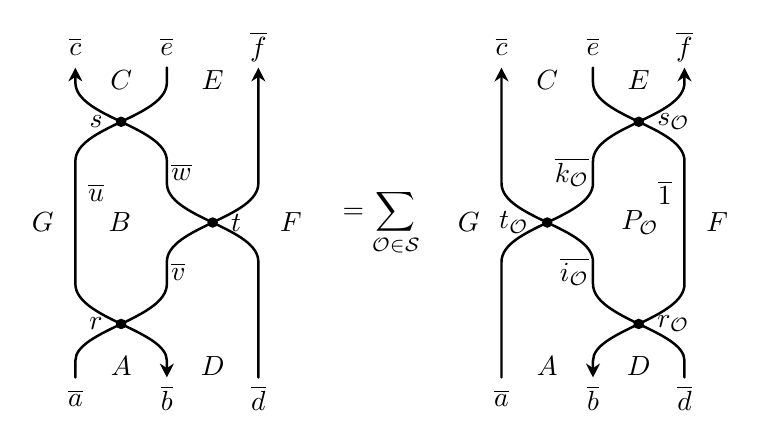
\begin{tikzpicture}[x=.83cm,y=.82cm]
\mixedThreeWires{arrowatend}{arrowatstart}{arrowatend}
\node[region] at (-0.5,2.4) {$G$};
\node[region] at (0.7,0.18) {$A$};
\node[region] at (2.1,0.18) {$D$};
\node[region] at (0.7,4.6) {$C$};
\node[region] at (2.1,4.6) {$E$};
\node[region] at (3.3,2.4) {$F$};
\node[strandlabel] at (0,-0.32) {$\overline{a}$};
\node[strandlabel] at (1.4,-0.32) {$\overline{b}$};
\node[strandlabel] at (2.8,-0.32) {$\overline{d}$};
\node[strandlabel] at (0,5.12) {$\overline{c}$};
\node[strandlabel] at (1.4,5.12) {$\overline{e}$};
\node[strandlabel] at (2.8,5.12) {$\overline{f}$};
\node[region] at (0.68,2.4) {$B$};
\fill (0.7,0.82875) circle (1.9pt);
\node[strandlabel,anchor=east] at (0.48,0.82875) {$r$};
\fill (2.1,2.4) circle (1.9pt);
\node[strandlabel,anchor=west] at (2.32,2.4) {$t$};
\fill (0.7,3.96) circle (1.9pt);
\node[strandlabel,anchor=east] at (0.48,3.96) {$s$};
\node[strandlabel,anchor=west] at (0.13,2.86) {$\overline{u}$};
\node[strandlabel,anchor=west] at (1.4,1.64) {$\overline{v}$};
\node[strandlabel,anchor=west] at (1.4,3.18) {$\overline{w}$};
\node at (4.68,2.4) {$=\displaystyle\sum_{\mathcal O\in\mathcal S}$};
\begin{scope}[shift={(6.52,0)}]
\begin{scope}[shift={(2.8,0)},xscale=-1]
\mixedThreeWires{arrowatend}{arrowatstart}{arrowatend}
\end{scope}
\node[region] at (-0.5,2.4) {$G$};
\node[region] at (0.7,0.18) {$A$};
\node[region] at (2.1,0.18) {$D$};
\node[region] at (0.7,4.6) {$C$};
\node[region] at (2.1,4.6) {$E$};
\node[region] at (3.3,2.4) {$F$};
\node[strandlabel] at (0,-0.32) {$\overline{a}$};
\node[strandlabel] at (1.4,-0.32) {$\overline{b}$};
\node[strandlabel] at (2.8,-0.32) {$\overline{d}$};
\node[strandlabel] at (0,5.12) {$\overline{c}$};
\node[strandlabel] at (1.4,5.12) {$\overline{e}$};
\node[strandlabel] at (2.8,5.12) {$\overline{f}$};
\node[region] at (2.12,2.4) {$P_{\mathcal O}$};
\fill (2.1,0.82875) circle (1.9pt);
\node[strandlabel,anchor=west] at (2.32,0.82875) {$r_{\mathcal O}$};
\fill (0.7,2.4) circle (1.9pt);
\node[strandlabel,anchor=east] at (0.48,2.4) {$t_{\mathcal O}$};
\fill (2.1,3.96) circle (1.9pt);
\node[strandlabel,anchor=west] at (2.32,3.96) {$s_{\mathcal O}$};
\node[strandlabel,anchor=east] at (2.67,2.86) {$\overline{1}$};
\node[strandlabel,anchor=east] at (1.4,1.64) {$\overline{i_{\mathcal O}}$};
\node[strandlabel,anchor=east] at (1.4,3.18) {$\overline{k_{\mathcal O}}$};
\end{scope}
\end{tikzpicture}
\end{center}

For linear left dots, expand into group-element triples and apply
the coefficient-one identity to each term. Any right orbit can
still be realized over \(\C\) with coefficient \(1\) by dividing
by its least multiplicity.

\begin{center}
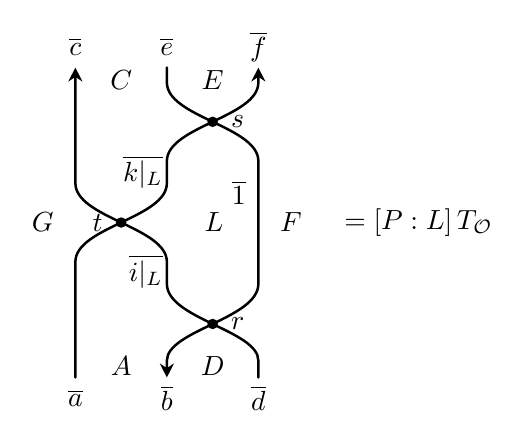
\begin{tikzpicture}[x=.83cm,y=.82cm]
\begin{scope}[shift={(2.8,0)},xscale=-1]
\mixedThreeWires{arrowatend}{arrowatstart}{arrowatend}
\end{scope}
\node[region] at (-0.5,2.4) {$G$};
\node[region] at (0.7,0.18) {$A$};
\node[region] at (2.1,0.18) {$D$};
\node[region] at (0.7,4.6) {$C$};
\node[region] at (2.1,4.6) {$E$};
\node[region] at (3.3,2.4) {$F$};
\node[strandlabel] at (0,-0.32) {$\overline{a}$};
\node[strandlabel] at (1.4,-0.32) {$\overline{b}$};
\node[strandlabel] at (2.8,-0.32) {$\overline{d}$};
\node[strandlabel] at (0,5.12) {$\overline{c}$};
\node[strandlabel] at (1.4,5.12) {$\overline{e}$};
\node[strandlabel] at (2.8,5.12) {$\overline{f}$};
\node[region] at (2.12,2.4) {$L$};
\fill (2.1,0.82875) circle (1.9pt);
\node[strandlabel,anchor=west] at (2.32,0.82875) {$r$};
\fill (0.7,2.4) circle (1.9pt);
\node[strandlabel,anchor=east] at (0.48,2.4) {$t$};
\fill (2.1,3.96) circle (1.9pt);
\node[strandlabel,anchor=west] at (2.32,3.96) {$s$};
\node[strandlabel,anchor=east] at (2.67,2.86) {$\overline{1}$};
\node[strandlabel,anchor=east] at (1.4,1.64) {$\overline{i|_L}$};
\node[strandlabel,anchor=east] at (1.4,3.18) {$\overline{k|_L}$};
\node at (5.25,2.4) {$=[P:L]\,T_{\mathcal O}$};
\end{tikzpicture}
\end{center}

\begin{proposition}[A Case 6 obstruction and a replacement family]\label{prop:parabolic-three-case-six}
If the projected pair stabilizer of a right orbit is strictly
smaller than the intersection of its two individual stabilizer
projections, its orbit map has no left replacement, even by a
finite sum.

On the other hand, suppose \(F=1\), all boundary embeddings are
inclusions, \(GE\) is a subgroup, \(D\cap GE=A\), and
\(G\cap E=C\). Then every right diagram has a single left
replacement through the parabolic group
\(\langle G\cup D\cup E\rangle\).
\end{proposition}

\begin{proof}
Proposition~\ref{prop:parabolic-three-unscaled} shows that a
group-element left term can have a nonzero coefficient on an
orbit only when its projected pair stabilizer equals the
intersection of the two individual projections. Every left
term therefore vanishes on the indicated orbit.

For the second assertion, \(B'=1\) on the right since \(F=1\).
For right dots \((r,t,s)\), take the displayed join as \(B\) on
the left, the inclusion embeddings, and dots
\((1,r^{-1}ts,1)\). In the left formula an output exists exactly
when \(xr^{-1}\in GE\), because \(g,t,s\in GE\). As
\(xr^{-1}\in D\), this is \(xr^{-1}\in A\).
In that case the class \([g(xr^{-1})t,s]_C\) is the unique
output, because \(G\cap E=C\). The right formula gives the same class
under the same condition. For linear right dots with coefficients
\(c_r,c_t,c_s\) at the three vertices, put
\(\sum_{r,t,s}c_r c_t c_s r^{-1}ts\) at the middle left dot. Every term is admissible because \(F=1\).
\end{proof}

\begin{center}
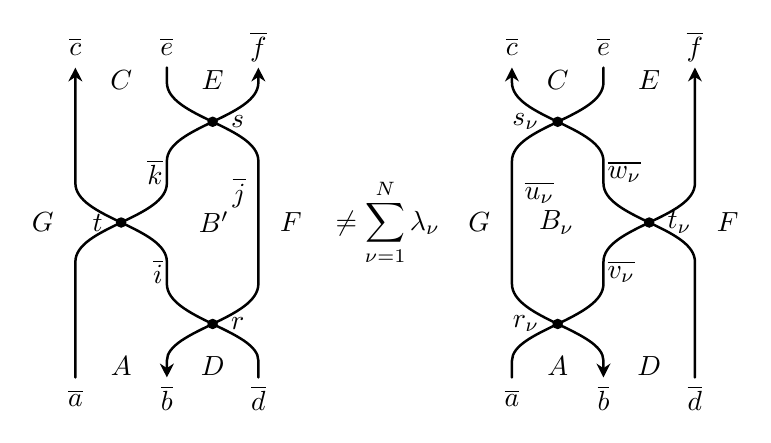
\begin{tikzpicture}[x=.83cm,y=.82cm]
\begin{scope}[shift={(2.8,0)},xscale=-1]
\mixedThreeWires{arrowatend}{arrowatstart}{arrowatend}
\end{scope}
\node[region] at (-0.5,2.4) {$G$};
\node[region] at (0.7,0.18) {$A$};
\node[region] at (2.1,0.18) {$D$};
\node[region] at (0.7,4.6) {$C$};
\node[region] at (2.1,4.6) {$E$};
\node[region] at (3.3,2.4) {$F$};
\node[strandlabel] at (0,-0.32) {$\overline{a}$};
\node[strandlabel] at (1.4,-0.32) {$\overline{b}$};
\node[strandlabel] at (2.8,-0.32) {$\overline{d}$};
\node[strandlabel] at (0,5.12) {$\overline{c}$};
\node[strandlabel] at (1.4,5.12) {$\overline{e}$};
\node[strandlabel] at (2.8,5.12) {$\overline{f}$};
\node[region] at (2.12,2.4) {$B'$};
\fill (2.1,0.82875) circle (1.9pt);
\node[strandlabel,anchor=west] at (2.32,0.82875) {$r$};
\fill (0.7,2.4) circle (1.9pt);
\node[strandlabel,anchor=east] at (0.48,2.4) {$t$};
\fill (2.1,3.96) circle (1.9pt);
\node[strandlabel,anchor=west] at (2.32,3.96) {$s$};
\node[strandlabel,anchor=east] at (2.67,2.86) {$\overline{j}$};
\node[strandlabel,anchor=east] at (1.4,1.64) {$\overline{i}$};
\node[strandlabel,anchor=east] at (1.4,3.18) {$\overline{k}$};
\node at (4.78,2.4) {$\ne\displaystyle\sum_{\nu=1}^{N}\lambda_\nu$};
\begin{scope}[shift={(6.68,0)}]
\mixedThreeWires{arrowatend}{arrowatstart}{arrowatend}
\node[region] at (-0.5,2.4) {$G$};
\node[region] at (0.7,0.18) {$A$};
\node[region] at (2.1,0.18) {$D$};
\node[region] at (0.7,4.6) {$C$};
\node[region] at (2.1,4.6) {$E$};
\node[region] at (3.3,2.4) {$F$};
\node[strandlabel] at (0,-0.32) {$\overline{a}$};
\node[strandlabel] at (1.4,-0.32) {$\overline{b}$};
\node[strandlabel] at (2.8,-0.32) {$\overline{d}$};
\node[strandlabel] at (0,5.12) {$\overline{c}$};
\node[strandlabel] at (1.4,5.12) {$\overline{e}$};
\node[strandlabel] at (2.8,5.12) {$\overline{f}$};
\node[region] at (0.68,2.4) {$B_\nu$};
\fill (0.7,0.82875) circle (1.9pt);
\node[strandlabel,anchor=east] at (0.48,0.82875) {$r_\nu$};
\fill (2.1,2.4) circle (1.9pt);
\node[strandlabel,anchor=west] at (2.32,2.4) {$t_\nu$};
\fill (0.7,3.96) circle (1.9pt);
\node[strandlabel,anchor=east] at (0.48,3.96) {$s_\nu$};
\node[strandlabel,anchor=west] at (0.13,2.86) {$\overline{u_\nu}$};
\node[strandlabel,anchor=west] at (1.4,1.64) {$\overline{v_\nu}$};
\node[strandlabel,anchor=west] at (1.4,3.18) {$\overline{w_\nu}$};
\end{scope}
\end{tikzpicture}
\end{center}


\begin{center}
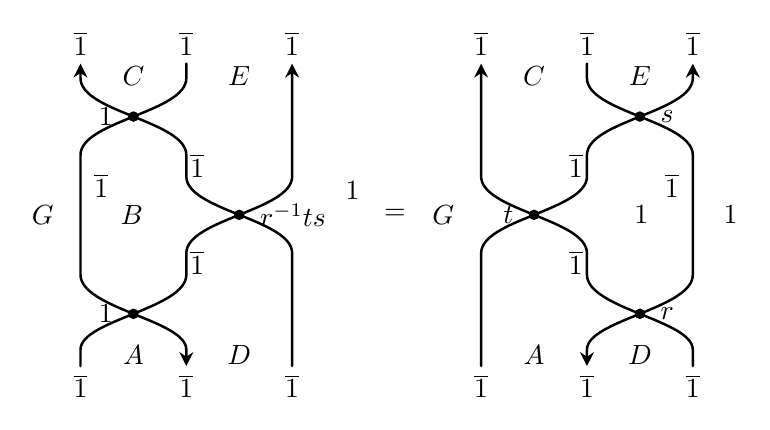
\begin{tikzpicture}[x=.96cm,y=.80cm]
\mixedThreeWires{arrowatend}{arrowatstart}{arrowatend}
\node[region] at (-0.5,2.4) {$G$};
\node[region] at (0.7,0.18) {$A$};
\node[region] at (2.1,0.18) {$D$};
\node[region] at (0.7,4.6) {$C$};
\node[region] at (2.1,4.6) {$E$};
\node[region] at (3.60,2.78) {$1$};
\node[strandlabel] at (0,-0.32) {$\overline{1}$};
\node[strandlabel] at (1.4,-0.32) {$\overline{1}$};
\node[strandlabel] at (2.8,-0.32) {$\overline{1}$};
\node[strandlabel] at (0,5.12) {$\overline{1}$};
\node[strandlabel] at (1.4,5.12) {$\overline{1}$};
\node[strandlabel] at (2.8,5.12) {$\overline{1}$};
\node[region] at (0.68,2.4) {$B$};
\fill (0.7,0.82875) circle (1.9pt);
\node[strandlabel,anchor=east] at (0.48,0.82875) {$1$};
\fill (2.1,2.4) circle (1.9pt);
\node[strandlabel,anchor=west] at (2.32,2.4) {$r^{-1}ts$};
\fill (0.7,3.96) circle (1.9pt);
\node[strandlabel,anchor=east] at (0.48,3.96) {$1$};
\node[strandlabel,anchor=west] at (0.13,2.86) {$\overline{1}$};
\node[strandlabel,anchor=west] at (1.4,1.64) {$\overline{1}$};
\node[strandlabel,anchor=west] at (1.4,3.18) {$\overline{1}$};
\node at (4.16,2.4) {$=$};
\begin{scope}[shift={(5.3,0)}]
\begin{scope}[shift={(2.8,0)},xscale=-1]
\mixedThreeWires{arrowatend}{arrowatstart}{arrowatend}
\end{scope}
\node[region] at (-0.5,2.4) {$G$};
\node[region] at (0.7,0.18) {$A$};
\node[region] at (2.1,0.18) {$D$};
\node[region] at (0.7,4.6) {$C$};
\node[region] at (2.1,4.6) {$E$};
\node[region] at (3.3,2.4) {$1$};
\node[strandlabel] at (0,-0.32) {$\overline{1}$};
\node[strandlabel] at (1.4,-0.32) {$\overline{1}$};
\node[strandlabel] at (2.8,-0.32) {$\overline{1}$};
\node[strandlabel] at (0,5.12) {$\overline{1}$};
\node[strandlabel] at (1.4,5.12) {$\overline{1}$};
\node[strandlabel] at (2.8,5.12) {$\overline{1}$};
\node[region] at (2.12,2.4) {$1$};
\fill (2.1,0.82875) circle (1.9pt);
\node[strandlabel,anchor=west] at (2.32,0.82875) {$r$};
\fill (0.7,2.4) circle (1.9pt);
\node[strandlabel,anchor=east] at (0.48,2.4) {$t$};
\fill (2.1,3.96) circle (1.9pt);
\node[strandlabel,anchor=west] at (2.32,3.96) {$s$};
\node[strandlabel,anchor=east] at (2.67,2.86) {$\overline{1}$};
\node[strandlabel,anchor=east] at (1.4,1.64) {$\overline{1}$};
\node[strandlabel,anchor=east] at (1.4,3.18) {$\overline{1}$};
\end{scope}
\end{tikzpicture}
\end{center}

\begin{example}[An orbit coefficient vanishing in characteristic three]\label{ex:case-six-characteristic-three}
Take all six boundary groups equal to
\(S_3\), the identity embeddings, and right dots \((1,(123),1)\)
with \(B'=1\). The individual projections are both \(S_3\),
while the pair stabilizer projects to \(\langle(123)\rangle\).
On the two bases identified with \(S_3\), the map sends
\(x\) to \(3x((123)+(132))\), since each conjugate of \((123)\)
is counted three times. Over a ring of characteristic \(3\), every
right diagram has zero coefficient on this orbit.
\end{example}

A left replacement can also fail when the projected pair stabilizer
equals the intersection of the two individual projections.

\begin{proposition}[A Case 6 obstruction with trivial projected stabilizer]\label{prop:parabolic-mixed-three}
A right diagram in the finite-parabolic category can have no left
replacement even when its projected pair stabilizer and both
individual stabilizer projections are trivial.
\end{proposition}

\begin{proof}


Example~\ref{ex:case-six-trivial-stabilizers} gives the obstruction. All three projected stabilizers are trivial because \(F=1\).
\end{proof}

\begin{example}[A Case 6 obstruction with trivial projected stabilizers]\label{ex:case-six-trivial-stabilizers}
Take
\[
 G=A=C=\langle(12),(34)\rangle,\qquad
 D=E=\operatorname{Sym}(\{1,2,3,4\}),\qquad F=1
\]
with inclusion embeddings. The two boundary bases identify with
\(D\) by multiplication. The right diagram with \(B'=1\) and unit
dots fixes the basis elements of \(A\) and sends those in
\(D\setminus A\) to zero by \eqref{eq:three-right-middle-restriction}.

Consider any left diagram with group-element dots \(r,t,s\) and
embeddings \(u,v,w\) as in Lemma~\ref{lem:three-middle-restriction}.
Its lower and upper vertex conditions give
\[
 u(G)\le r v(D)r^{-1},\qquad u(G)\le s w(E)s^{-1}.
\]
The image \(u(G)\) moves four points. Both displayed overgroups are
full symmetric groups on four points, so they are the same subgroup.
Use \([1,x]_A\) and \([1,y]_C\) for the input and output.
The left-diagram equation becomes
\[
 s w(y)s^{-1}=(r v(x)r^{-1})(rts^{-1}).
\]
If \(rts^{-1}\) belongs to the common subgroup, every input has
exactly one output. Otherwise every input has zero outputs.
By linearity, the sum of the output coefficients of any finite
sum of left diagrams is constant on basis inputs. The right
diagram has coefficient sum \(1\) on \(A\) and \(0\) off \(A\),
so it has no left replacement.

\end{example}


\begin{example}[A left replacement through overlapping blocks]\label{ex:case-six-overlap}
Take
\(G=A=C=F=1\), \(D=\langle(12)\rangle\) and
\(E=\langle(23)\rangle\). The right diagram that sends \(r\) to
\(s\) and all other basis elements to zero has a left
replacement with middle group \(\operatorname{Sym}(\{1,2,3\})\)
and middle dot \(r^{-1}s\).

\begin{center}
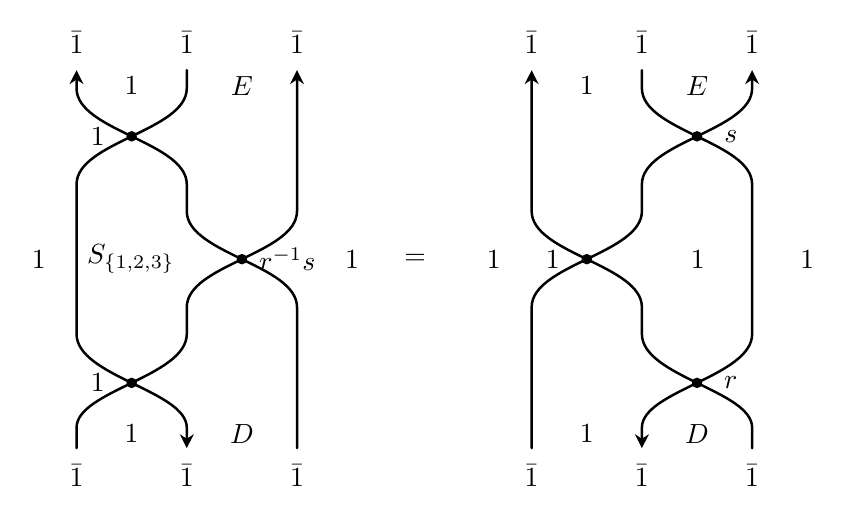
\begin{tikzpicture}[x=1cm,y=1cm]
\newcommand{\parabolicCaseSixBoundary}{%
  \node[region] at (-.48,2.4) {$1$};
  \node[region] at (3.50,2.4) {$1$};
  \node[region] at (.70,.18) {$1$};
  \node[region] at (2.10,.18) {$D$};
  \node[region] at (.70,4.60) {$1$};
  \node[region] at (2.10,4.60) {$E$};
  \foreach \x in {0,1.4,2.8} {%
    \node[strandlabel] at (\x,-.35) {$\bar1$};
    \node[strandlabel] at (\x,5.15) {$\bar1$};%
  }%
}
\mixedThreeWires{arrowatend}{arrowatstart}{arrowatend}
\parabolicCaseSixBoundary
\fill (.7,.82875) circle (1.9pt);
\fill (2.1,2.4) circle (1.9pt);
\fill (.7,3.96) circle (1.9pt);
\node[strandlabel] at (.27,.82875) {$1$};
\node[strandlabel,anchor=west] at (2.27,2.4) {$r^{-1}s$};
\node[strandlabel] at (.27,3.96) {$1$};
\node[region] at (.69,2.4) {$S_{\{1,2,3\}}$};
\node at (4.30,2.4) {$=$};
\begin{scope}[xshift=5.78cm]
  \begin{scope}[shift={(2.8,0)},xscale=-1]
    \mixedThreeWires{arrowatend}{arrowatstart}{arrowatend}
  \end{scope}
  \parabolicCaseSixBoundary
  \fill (2.1,.82875) circle (1.9pt);
  \fill (.7,2.4) circle (1.9pt);
  \fill (2.1,3.96) circle (1.9pt);
  \node[strandlabel] at (2.53,.82875) {$r$};
  \node[strandlabel] at (.27,2.4) {$1$};
  \node[strandlabel] at (2.53,3.96) {$s$};
  \node[region] at (2.11,2.4) {$1$};
\end{scope}
\end{tikzpicture}
\end{center}
\end{example}


\section*{AI usage disclosure}
Codex was used to test conjectures proposed by myself and verify the
correctness of my own handwritten proofs. The new results and
constructions are my own.

\begin{thebibliography}{9}
\bibitem{watts}
C.~E. Watts, \emph{Intrinsic characterizations of some additive functors},
Proc. Amer. Math. Soc. \textbf{11} (1960), 5--8.
\href{https://doi.org/10.2307/2032707}{doi:10.2307/2032707}.

\bibitem{getcurious}
Ian Xiao, \emph{Abelian Categories and Bimodules}.
Get Curious, 2026, Chapters 8--10.
\href{https://getcurious.cc/downloads/abelian-categories-and-bimodules-lecture-notes.pdf}{Collected notes}.

\bibitem{mackey}
G.~W. Mackey, \emph{On induced representations of groups},
Amer. J. Math. \textbf{73} (1951), 576--592.
\href{https://doi.org/10.2307/2372309}{doi:10.2307/2372309}.

\bibitem{james-kerber}
G.~James and A.~Kerber, \emph{The Representation Theory of the Symmetric
Group}, Addison-Wesley, 1981, Section~1.3.
\href{https://www.cambridge.org/core/books/abs/representation-theory-of-the-symmetric-group/symmetric-groups-and-their-young-subgroups/F308612FED7EEF675EB29ED670C6528E}{Chapter 1}.

\bibitem{khovanov}
M.~Khovanov, \emph{Heisenberg algebra and a graphical calculus},
Fund. Math. \textbf{225} (2014), 169--210.
\href{https://doi.org/10.4064/fm225-1-8}{doi:10.4064/fm225-1-8}.
\href{https://arxiv.org/abs/1009.3295}{arXiv:1009.3295}.

\end{thebibliography}
\end{document}

